
%=======================================================================
% riscv-interrupts.tex
%-----------------------------------------------------------------------

\documentclass[twoside,11pt]{book}

% Fix copy/pasting of ligatures in Acrobat
\input{glyphtounicode.tex}
\pdfgentounicode=1 %


%------------------------------------------------------------------------------
% Packages.
%------------------------------------------------------------------------------

\usepackage{graphicx}
\usepackage{colortbl}
\usepackage[svgnames]{xcolor}

\usepackage[colorlinks,citecolor=Navy,linkcolor=Navy]{hyperref}
\usepackage{placeins}
\usepackage{enumitem}

%------------------------------------------------------------------------------
% Main parameters.
%------------------------------------------------------------------------------

\setlength{\topmargin}{-0.5in}
\setlength{\textheight}{9in}
\setlength{\oddsidemargin}{0in}
\setlength{\evensidemargin}{0in}
\setlength{\textwidth}{6.5in}

\pagestyle{myheadings}
\setlength{\parindent}{0in}
\setlength{\parskip}{10pt}
\sloppy
\raggedbottom
\clubpenalty=10000
\widowpenalty=10000

\newlength{\defaultListTopsep}
\defaultListTopsep=0.25\parskip
\setlist{
	partopsep=0mm,
	topsep=\defaultListTopsep,
	itemsep=0mm,
	parsep=\parskip
}

\intextsep=2.5\parskip
\textfloatsep=2.5\parskip
\abovecaptionskip=0.25\parskip
\belowcaptionskip=-0.25\parskip

\renewcommand{\footnoterule}{%
	\vfill\kern\parskip
	\hrule width \textwidth height 1pt
	\kern 0.25\baselineskip
}

%------------------------------------------------------------------------------
% Custom list and table environments.
%------------------------------------------------------------------------------

\newlist{tightList}{itemize}{1}
\setlist[tightList]{label=\textbullet, nosep}

\newenvironment{displayLinesTable}[1][l]{%
	\par
	\vspace{\defaultListTopsep}%
	\noindent\begin{tabular}{@{\hspace{\leftmargin}}#1}%
}{%
	\end{tabular}\par
	\vspace{\defaultListTopsep}%
	\ignorespacesafterend
}

\newenvironment{commentary}{%
	\vspace{-1.5mm}
	\list{}{
		\topsep		0mm
		\partopsep	0mm
		\listparindent	1.5em
		\itemindent	\listparindent
		\rightmargin	\leftmargin
		\parsep		0mm
	}
	\item
	\small\em
	\noindent\nopagebreak\rule{\linewidth}{1pt}\par
	\noindent\ignorespaces
}{%
	\endlist
}

%------------------------------------------------------------------------------
% Commands for register format figures.
%------------------------------------------------------------------------------

% New column types to use in tabular environment for instruction formats.
% Allocate 0.18in per bit.
\newcolumntype{I}{>{\centering\arraybackslash}p{0.18in}}
% Two-bit centered column.
\newcolumntype{W}{>{\centering\arraybackslash}p{0.36in}}
% Three-bit centered column.
\newcolumntype{F}{>{\centering\arraybackslash}p{0.54in}}
% Four-bit centered column.
\newcolumntype{Y}{>{\centering\arraybackslash}p{0.72in}}
% Five-bit centered column.
\newcolumntype{R}{>{\centering\arraybackslash}p{0.9in}}
% Six-bit centered column.
\newcolumntype{S}{>{\centering\arraybackslash}p{1.08in}}
% Seven-bit centered column.
\newcolumntype{O}{>{\centering\arraybackslash}p{1.26in}}
% Eight-bit centered column.
\newcolumntype{E}{>{\centering\arraybackslash}p{1.44in}}
% Ten-bit centered column.
\newcolumntype{T}{>{\centering\arraybackslash}p{1.8in}}
% Twelve-bit centered column.
\newcolumntype{M}{>{\centering\arraybackslash}p{2.2in}}
% Sixteen-bit centered column.
\newcolumntype{K}{>{\centering\arraybackslash}p{2.88in}}
% Twenty-bit centered column.
\newcolumntype{U}{>{\centering\arraybackslash}p{3.6in}}
% Twenty-bit centered column.
\newcolumntype{L}{>{\centering\arraybackslash}p{3.6in}}
% Twenty-five-bit centered column.
\newcolumntype{J}{>{\centering\arraybackslash}p{4.5in}}

\newcommand{\instbit}[1]{\mbox{\scriptsize #1}}
\newcommand{\instbitrange}[2]{~\instbit{#1} \hfill \instbit{#2}~}
\newcommand{\reglabel}[1]{\hfill {\tt #1}\hfill\ }

%------------------------------------------------------------------------------
%------------------------------------------------------------------------------

\newcommand{\z}[1]{{\tt\catcode`\`=\active\protect\frenchspacing#1}}
\newcommand{\zSafe}[1]{{\tt #1}}
\newcommand{\LB}{\char123}
\newcommand{\RB}{\char125}
\newcommand{\RISCV}{\mbox{RISC-V}}

\newcommand{\WIRI}{\textbf{WIRI}}
\newcommand{\WPRI}{\textbf{WPRI}}
\newcommand{\WLRL}{\textbf{WLRL}}
\newcommand{\WARL}{\textbf{WARL}}

\newcommand{\unspecified}{\textsc{unspecified}}



\newcommand{\AIARev}{0.2-draft}
\newcommand{\AIAMonthYear}{Month YEAR}

\setcounter{secnumdepth}{3}
\setcounter{tocdepth}{3}

\renewcommand{\chaptermark}[1]{%
	\markboth{%
		RISC-V Advanced Interrupt Architecture V\AIARev%
			\hspace{1em}\rule{1ex}{1ex}%
	}{%
		\rule{1ex}{1ex}\hspace{1em}\chaptername\ \thechapter.\ #1%
	}%
}

%=======================================================================

\begin{document}

%=======================================================================

\title{%
  \vspace{-0.7in}%
  {\Large\bf The RISC-V Advanced Interrupt Architecture} \\
  {\large Document Version \AIARev}
  \vspace{-0.1in}%
}

\author{%
  Editor: John Hauser \\
  {\tt jh.riscv\mbox{}@jhauser.us} \\
  \\
  \today
}

\date{}
\maketitle

\thispagestyle{empty}

Contributors to all versions of this specification in alphabetical
order (please contact the editor to suggest corrections):
Krste Asanovi\'{c},
Greg Favor,
John Hauser,
David Kruckemyer,
Shubu Mukherjee,
Anup Patel,
Josh Scheid,
and Andrew Waterman.

This document is released under a Creative Commons Attribution 4.0
International License.

%=======================================================================

\frontmatter

{\hypersetup{linktoc=all,hidelinks}
\tableofcontents
}

%=======================================================================

\mainmatter


%=======================================================================
\chapter{Introduction}
\label{ch:intro}

\textbf{%
This chapter is \emph{frozen}, meaning
a functional change is extremely unlikely.
Change will occur only because of some truly critical issue
being identified during public review.%
}
\bigskip

This document specifies the Advanced Interrupt Architecture for
{\RISCV}, consisting of:
(a)~an extension to the standard Privileged Architecture for {\RISCV}
harts specified in Volume~II of The {\RISCV} Instruction Set Manual;
(b)~two standard interrupt controllers for {\RISCV} systems, an
Advanced Platform-Level Interrupt Controller (APLIC) and an
Incoming Message-Signaled Interrupt Controller (IMSIC); and
(c)~requirements on other system components concerning interrupts.

\begin{commentary}
Commentary on our design decisions, implementation options, and
application is formatted as in this paragraph, and can be skipped if
the reader is only interested in the specification itself.
\end{commentary}

%-----------------------------------------------------------------------
\section{Goals}

The {\RISCV} Advanced Interrupt Architecture has these goals:
\begin{itemize}

\item
Build upon the interrupt-handling functionality of the {\RISCV}
Privileged Architecture, minimizing the replacement of existing
functionality.

\item
Provide facilities for {\RISCV} systems to work directly with
message-signaled interrupts (MSIs) as employed by PCI Express and other
device standards, in addition to basic wired interrupts.

\item
For wired interrupts, define a new Platform-Level Interrupt Controller
(the Advanced PLIC, or APLIC)
that has an independent control interface for each
level of privilege (such as {\RISCV} machine and supervisor levels),
and that can convert wired interrupts into MSIs for systems supporting
MSIs.

\item
Expand the framework for local interrupts at a {\RISCV} hart.

\item
Optionally allow software to configure the relative priorities of all
sources of interrupts to a {\RISCV} hart (including the standard timer
and software interrupts, among others), instead of being limited
just to the ability of a separate interrupt controller to prioritize
external interrupts only.

\item
When harts implement the Privileged Architecture's hypervisor
extension, provide sufficient assistance for virtualizing these same
interrupt facilities for virtual machines.

\item
With the help of an \mbox{IOMMU} (I/O memory management unit) for redirecting
MSIs, maximize the opportunities and ability for a guest operating
system running in a virtual machine to have direct control of devices
with minimal involvement of a hypervisor.

\item
Avoid having the interrupt hardware be a limiter on the number of
virtual machines.

\item
Achieve all of the above with the best possible compromises between
speed, efficiency, and flexibility of implementation.

\end{itemize}

This initial version of the Advanced Interrupt Architecture is focused
primarily on the needs of larger, high-performance {\RISCV} systems.
Support is not currently defined for the following interrupt-handling
features that are useful for minimizing interrupt response times in
so-called ``real-time'' systems but are less appropriate for high-speed
processor cores:
\begin{tightList}
\item
the option to give each interrupt source at a hart a separate trap
entry address;
\item
automatic stacking of register values on interrupt trap entry, and
restoration on exit; and
\item
automatic preemption (nesting) of interrupts at a hart, based on
priority.
\end{tightList}
It is intended that such features optimizing for smaller and/or
real-time systems can be developed as a follow-on extension, either
separately or as part of a future version of the interrupt architecture
of this document.

%-----------------------------------------------------------------------
\section{Limits}

In its current version, the {\RISCV} Advanced Interrupt Architecture
can support {\RISCV} symmetric multiprocessing (SMP) systems with up to
16,384 harts.
If the harts are \mbox{64-bit} (RV64) and implement the hypervisor
extension, and if all features of the Advanced Interrupt Architecture
are fully implemented as well, then for each physical hart there may be
up to 63 active virtual harts and potentially thousands of additional
idle (swapped-out) virtual harts, where each virtual hart has direct
control of one or more physical devices.

Table~\ref{tab:overallLimits} summarizes the main limits on the numbers
of harts, both physical and virtual, and the numbers of distinct
interrupt identities that may be supported with the Advanced Interrupt
Architecture.

\begin{table*}[h!]
\begin{center}
\begin{tabular}{|l|c|l|}
\hline
   & Maximum      & \multicolumn{1}{c|}{Requirements} \\
\hline
\hline
Physical harts
   & 16,384       & \\
\hline
Active virtual harts having direct control of \quad
   & 31 for RV32, & {\RISCV} hypervisor extension; \\
\ a device, per physical hart
   & 63 for RV64  & \ IMSICs with guest interrupt\\
   &              & \ files; and an IOMMU \\
\hline
Idle (swapped-out) virtual harts having \quad
   & potentially  & An IOMMU with support \\
\ direct control of a device, per physical hart \quad
   & thousands    & \ for memory-resident \\
   &              & \ interrupt files \\
\hline
Wired interrupts at a single APLIC \quad
   & 1023         & \\
\hline
Distinct identities usable for MSIs at each \quad
   & 2047         & IMSICs \\
\ hart (physical or virtual)
   &              & \\
\hline
\end{tabular}
\end{center}
\caption{%
Absolute limits on the numbers of harts and interrupt identities in a
system.
Individual implementations are likely to have smaller limits.%
}
\label{tab:overallLimits}
\end{table*}

\begin{commentary}
We assume that any single {\RISCV} computer (or any single node in a
cluster or distributed system) with many thousands of physical harts
will probably need an interrupt infrastructure adapted to the machine's
specific organization, which we do not attempt to predict.
\end{commentary}

%-----------------------------------------------------------------------
\section{Overview of main components}

A {\RISCV} system's overall architecture for signaling interrupts
depends on whether it is built mainly for message-signaled interrupts
(MSIs) or for more traditional wired interrupts.
In systems with full support for MSIs, every hart has an
\emph{Incoming MSI Controller} (IMSIC) that serves as the hart's own
private interrupt controller for external interrupts.
Conversely, in systems based primarily on traditional wired interrupts,
harts do not have IMSICs.
Larger systems, and especially those with PCI devices, are
expected to fully support MSIs by giving harts IMSICs, whereas many
smaller systems may continue to be best served with wired interrupts
and simpler harts without IMSICs.

%- - - - - - - - - - - - - - - - - - - - - - - - - - - - - - - - - - - -
\subsection{External interrupts without IMSICs}

When {\RISCV} harts do not have Incoming MSI Controllers, external
interrupts are signaled to harts through dedicated wires.
In that case, an \emph{Advanced Platform-Level Interrupt Controller}
(APLIC) acts as a traditional central hub for interrupts,
routing and prioritizing external interrupts for each hart as
illustrated in Figure~\ref{fig:intrsWithoutIMSICs}.
Interrupts may be selectively routed either to machine level or to
supervisor level at each hart.
The APLIC is specified in Chapter~\ref{ch:AdvPLIC}.

\begin{figure}[th]
\centerline{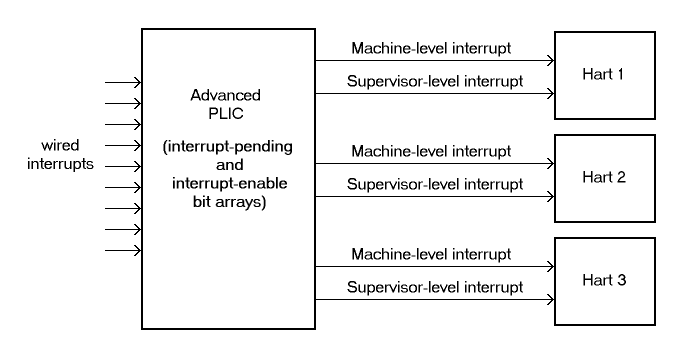
\includegraphics[scale=0.55]{intrsWithoutIMSICs.png}}
\caption{%
Traditional delivery of wired interrupts to harts without support for
MSIs.%
}
\label{fig:intrsWithoutIMSICs}
\end{figure}

Without IMSICs, the current Advanced Interrupt Architecture does
not support the direct signaling of external interrupts to virtual
machines, even when {\RISCV} harts implement the Privileged
Architecture's hypervisor extension.
Instead, an interrupt must be sent to the relevant hypervisor, which
can then choose to inject a virtual interrupt into the virtual machine.

\begin{commentary}
If harts implement the hypervisor extension, it is a topic of ongoing
study whether an APLIC should be allowed to route external
interrupts to be the \emph{guest external interrupts} of the hypervisor
extension, permitting the delivery of interrupts directly to virtual
machines without the need for each signaled interrupt to be handled at
the hypervisor level.
For now, we assume that systems that need direct signaling of external
interrupts to virtual machines will have IMSICs.
\end{commentary}

\begin{figure}[th]
\centerline{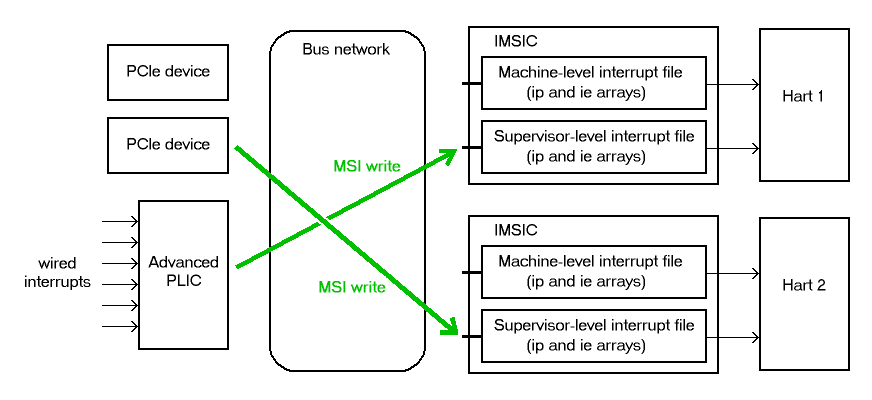
\includegraphics[scale=0.55]{intrsWithIMSICs.png}}
\caption{%
Interrupt delivery by MSIs when harts have IMSICs for receiving them.%
}
\label{fig:intrsWithIMSICs}
\end{figure}

%*** REMOVE?:
\FloatBarrier

%- - - - - - - - - - - - - - - - - - - - - - - - - - - - - - - - - - - -
\subsection{External interrupts with IMSICs}

To be able to receive message-signaled interrupts (MSIs), each
{\RISCV} hart must have an Incoming MSI Controller (IMSIC) as shown in
Figure~\ref{fig:intrsWithIMSICs}.
Fundamentally, a message-signaled interrupt is simply a memory write to
a specific address that hardware accepts as indicating an interrupt.
To that end, every IMSIC is assigned one or more distinct addresses in
the machine's address space, and when a write is made to one of those
addresses in the expected format, the receiving IMSIC interprets the
write as an external interrupt for the respective hart.

Because all IMSICs have unique addresses in the machine's physical
address space, every IMSIC can receive MSI writes from any agent (hart
or device) with permission to write to it.
IMSICs have separate addresses for MSIs directed to machine and
supervisor levels, in part so the ability to signal interrupts at each
privilege level can be separately granted or denied by controlling
write permissions at the different addresses, and in part to better
support virtualizability (pretending that one privilege level is a
higher level).
MSIs intended for a hart at a specific privilege level are recorded
within the IMSIC in an \emph{interrupt file}, which consists mainly
of an array of interrupt-pending bits and a matching array of
interrupt-enable bits, the latter indicating which individual
interrupts the hart is currently prepared to receive.

IMSIC units are fully defined in Chapter~\ref{ch:IMSIC}.
The format of MSIs used by the {\RISCV} Advanced Interrupt Architecture
is described in that chapter, Section~\ref{sec:MSIEncoding}.

When the harts in a {\RISCV} system have IMSICs, the system will
normally still contain an APLIC, but its role is changed.
Instead of signaling interrupts to harts directly by wires as in
Figure~\ref{fig:intrsWithoutIMSICs}, an APLIC converts incoming
wired interrupts into MSI writes that are sent to harts via their IMSIC
units.
Each MSI is sent to a single target hart according to the APLIC's
configuration set by software.

If {\RISCV} harts implement the Privileged Architecture's hypervisor
extension, IMSICs may have additional \emph{guest interrupt files} for
delivering interrupts to virtual machines.
Besides Chapter~\ref{ch:IMSIC} on the IMSIC, see
Chapter~\ref{ch:VSLevel} which specifically covers interrupts to
virtual machines.
If the system also contains an \mbox{IOMMU} to perform address translation
of memory accesses made by I/O devices, then MSIs from those same
devices may require special handling.
This topic is addressed in Chapter~\ref{ch:IOMMU}, ``\mbox{IOMMU} Support
for MSIs to Virtual Machines.''

%- - - - - - - - - - - - - - - - - - - - - - - - - - - - - - - - - - - -
\subsection{Other interrupts}

In addition to external interrupts from I/O devices, the {\RISCV}
Privileged Architecture specifies a few other major classes of
interrupts for harts.
The Privileged Architecture's timer interrupts remain supported
in full, and software interrupts remain at least partly supported,
although neither appears in Figures \ref{fig:intrsWithoutIMSICs}
and~\ref{fig:intrsWithIMSICs}.
For the specifics on software interrupts, refer to
Chapter~\ref{ch:IPIs}, ``Interprocessor Interrupts (IPIs).''

The Advanced Interrupt Architecture adds considerable support
for \emph{local interrupts} at a hart, whereby a hart essentially
interrupts itself in response to asynchronous events, usually errors.
Local interrupts remain contained within a hart (or close to it),
so like standard {\RISCV} timer and software interrupts, they do not
pass through an APLIC or IMSIC.

%-----------------------------------------------------------------------
\section{Interrupt identities at a hart}

The {\RISCV} Privileged Architecture gives every interrupt cause at a
hart a distinct \emph{major identity number}, which is the Exception
Code automatically written to CSR \z{mcause} or \z{scause} on an
interrupt trap.
Interrupt causes that are standardized by the Privileged Architecture
have major identities in the range 0--15, while numbers 16 and higher
are officially available for platform standards or for custom use.
The Advanced Interrupt Architecture claims further authority over
identity numbers in the ranges 16--23 and 32--47, leaving numbers in the
range 24--31 and all major identities 48 and higher still free for custom
use.
Table~\ref{tab:interruptIdents} characterizes all major interrupt
identities with this extension.

\begin{table*}[h!]
\begin{center}
\begin{tabular}{|c|c|l|}
\hline
Major identity & Minor identity & \\
\hline
\hline
0              & --             & \em Reserved by Privileged Architecture \\
\hline
1              & --             & Supervisor software interrupt \\
2              & --             & Virtual supervisor software interrupt \\
3              & --             & Machine software interrupt \\
\hline
4              & --             & \em Reserved by Privileged Architecture \\
\hline
5              & --             & Supervisor timer interrupt \\
6              & --             & Virtual supervisor timer interrupt \\
7              & --             & Machine timer interrupt \\
\hline
8              & --             & \em Reserved by Privileged Architecture \\
\hline
9              & \multicolumn{1}{l|}{Determined by}
                                & Supervisor external interrupt \\
10             & \multicolumn{1}{l|}{\ external interrupt}
                                & Virtual supervisor external interrupt \\
11             & \multicolumn{1}{l|}{\ controller}
                                & Machine external interrupt \\
\hline
12                   & -- & Supervisor guest external interrupt \\
13                   & -- & Counter overflow interrupt \\
14--15               & -- & \em Reserved by Privileged Architecture \\
\hline
\hline
16--23         & --       & \em Reserved for standard local interrupts \\
24--31         & --       & \em Designated for custom use \\
32--47         & --       & \em Reserved for standard local interrupts \\
$\geq \mbox{48}$ & --     & \em Designated for custom use \\
\hline
\end{tabular}
\end{center}
\caption{%
Major and minor identities for all interrupt causes at a hart.
Major identities 0--15 are the purview of the {\RISCV} Privileged
Architecture.%
}
\label{tab:interruptIdents}
\end{table*}

Interrupts from most I/O devices are conveyed to a hart by the
\emph{external interrupt controller} for the hart, which is either the
hart's IMSIC (Figure~\ref{fig:intrsWithIMSICs}) or an APLIC
(Figure~\ref{fig:intrsWithoutIMSICs}).
As Table~\ref{tab:interruptIdents} shows, external interrupts
at a given privilege level all share a single major identity
number:  11~for machine level, 9~for supervisor level, and 10 for
\mbox{VS-level}.
External interrupts from different causes are distinguished from one
another at a hart by their \emph{minor identity numbers} supplied by
the external interrupt controller.

Other interrupt causes besides external interrupts might also have
their own minor identities.
However, this document has need to discuss minor identities only with
regard to external interrupts.

The local interrupts defined by the Advanced Interrupt Architecture
and their handling are covered mainly in Chapter~\ref{ch:MSLevel},
``Interrupts for Machine and Supervisor Levels.''

%-----------------------------------------------------------------------
\section{Selection of harts to receive an interrupt}

Each signaled interrupt is delivered to only one hart at one privilege
level, usually determined by software in one way or another.
Unlike some other architectures, the {\RISCV} Advanced Interrupt
Architecture provides no standard hardware mechanism for the broadcast
or multicast of interrupts to multiple harts.

For local interrupts, and for any ``virtual'' interrupts that software
injects into lower privilege levels at a hart, the interrupts are
entirely a local affair at the hart and are never visible to other
harts.
The {\RISCV} Privileged Architecture's timer interrupts are also
uniquely tied to individual harts.
For other interrupts, received by a hart from sources outside the
hart, each interrupt signal (whether delivered by wire or by an MSI) is
configured by software to go to only a single hart.

To send an interprocessor interrupt (IPI) to multiple harts, the
originating hart need only execute a loop, sending an individual IPI to
each destination hart.
For IPIs to a single destination hart, see Chapter~\ref{ch:IPIs}.

\begin{commentary}
The effort that a source hart expends in sending individual IPIs to
multiple destinations will invariably be dwarfed by the combined effort
at the receiving harts to handle those interrupts.
Hence, providing an automated mechanism for IPI multicast could be
expected to reduce a system's total overall work only modestly at best.
With a very large number of harts, a hardware mechanism for IPI
multicast must contend with the question of how exactly software
specifies the intended destination set with each use, and furthermore,
the actual physical delivery of IPIs may not differ that much from the
software version.

We do not exclude the future possibility of an optional hardware
mechanism for multicast IPI, but only if a significant advantage can be
demonstrated in real use.
As of 2020, Linux has been observed not to make use of multicast IPI
hardware even on systems that have it.
\end{commentary}

In the rare event that a single interrupt from an I/O device needs
to be communicated to multiple harts, the interrupt must be sent to a
single hart which can then signal the other harts by IPIs.

\begin{commentary}
We contend that the need to communicate an I/O interrupt to multiple
harts is sufficiently rare that standardizing hardware support for multicast
cannot be justified in this case.
\end{commentary}

\begin{commentary}
Along with multicast delivery, other architectures support an option
for ``\mbox{1-of-$N$}'' delivery of interrupts, whereby the hardware
chooses a single destination hart from among a configured set of
$N$ harts, with the goal of automatic load balancing of interrupt
handling among the harts.
Experiments in the 2010s called into question the utility of
\mbox{1-of-$N$} modes in practice, showing that software could often do
a better job of load balancing than the hardware algorithms implemented
in actual chips.
Linux was consequently modified to discontinue using \mbox{1-of-$N$}
interrupt delivery even on systems that have it.

We remain open to the argument that hardware load balancing of
interrupt handling may be beneficial for certain specialized markets,
such as networking.
However, the claims made so far in this regard do not justify requiring
support for \mbox{1-of-$N$} delivery in all {\RISCV} servers.
With more evidence, some mechanism for \mbox{1-of-$N$} delivery might
become a future option.
\end{commentary}

\begin{commentary}
The original Platform-Level Interrupt Controller (PLIC) for {\RISCV}
is configurable so each interrupt source signals external interrupts to
any subset of the harts, potentially all harts.
When multiple harts receive an external interrupt from a single cause
at the PLIC, the first hart to \emph{claim} the interrupt at the PLIC
is the one responsible for servicing it.
Usually this sets up a race, where the subset of harts configured to
receive the multicast interrupt all take an external interrupt trap
simultaneously and compete to be the first to claim the interrupt at
the PLIC.
The intention is to provide a form of \mbox{1-of-$N$} interrupt
delivery.
However, for all the harts that fail to win the claim, the interrupt
trap becomes wasted effort.

For the reasons already given, the Advanced PLIC supports sending each
signaled interrupt to only a single hart chosen by software, not to
multiple harts.
\end{commentary}

%-----------------------------------------------------------------------
\section{ISA extensions Smaia and Ssaia}

The Advanced Interrupt Architecture (AIA) defines two names for
extensions to the {\RISCV} instruction set architecture (ISA),
one for machine-level execution environments,
and another for supervisor-level environments.
For a machine-level environment, extension \textbf{Smaia} encompasses
all added CSRs and all modifications to interrupt response behavior
that the AIA specifies for a hart, over all privilege levels.
For a supervisor-level environment, extension \textbf{Ssaia} is
essentially the same as Smaia except excluding the machine-level
CSRs and behavior not directly visible to supervisor level.

Extensions Smaia and Ssaia cover only
those AIA features that impact the ISA at a hart.
Although the following are described or discussed
in this document as part of the AIA, they are not implied by
Smaia or Ssaia because the components are categorized as non-ISA:
APLICs, Duo-PLICs, IOMMUs, and any mechanisms for initiating
interprocessor interrupts apart from writing to IMSICs.

As revealed in subsequent chapters, the exact set
of CSRs and behavior added by the AIA, and hence
implied by Smaia or Ssaia, depends on
the base ISA's XLEN (RV32 or RV64), on whether \mbox{S-mode}
and the hypervisor extension are implemented,
and on whether the hart has an IMSIC.
But individual AIA extension names are not
provided for each possible valid subset.
Rather, the different combinations are inferable
from the intersection of features indicated (such as
RV64I + \mbox{S-mode} + Smaia, but without the hypervisor extension).

Software development tools like compilers and assemblers need not
be concerned about whether an IMSIC exists but should just
allow attempts to access the IMSIC CSRs (described in Chapters
\ref{ch:CSRs} and~\ref{ch:IMSIC}) if Smaia or Ssaia is indicated.
Without an actual IMSIC, such attempts may trap,
but that is not a problem for the development tools.



%=======================================================================
\chapter{Control and Status Registers (CSRs) Added to Harts}
\label{ch:CSRs}
\chaptermark{CSRs Added to Harts}

\textbf{%
This chapter is \emph{frozen} and has already passed public review,
making a functional change at this stage extremely unlikely.%
}
\bigskip

For each privilege level at which a {\RISCV} hart can take interrupt
traps, the Advanced Interrupt Architecture adds CSRs for interrupt
control and handling.

%-----------------------------------------------------------------------
\section{Machine-level CSRs}

Table~\ref{tab:CSRs-M} lists both the CSRs added for machine level
and existing machine-level CSRs whose size is changed
by the Advanced Interrupt Architecture.
Existing CSRs \z{mie}, \z{mip}, and \z{mideleg} are
widended to 64~bits to support a total of 64 interrupt causes.

\begin{table*}[h!]
\begin{center}
\begin{tabular}{|c|c|c|l|l|}
\hline
Number & Privilege & Width & Name & Description \\
\hline
\hline
\multicolumn{5}{|c|}{Machine-Level Window to Indirectly Accessed Registers} \\
\hline
\z{0x350} & MRW & XLEN  & \z{miselect} & Machine indirect register select \\
\z{0x351} & MRW & XLEN  & \z{mireg}    & Machine indirect register alias \\
\hline
\multicolumn{5}{|c|}{Machine-Level Interrupts} \\
\hline
\z{0x304} & MRW & 64    & \z{mie}    & Machine interrupt-enable bits \\
\z{0x344} & MRW & 64    & \z{mip}    & Machine interrupt-pending bits \\
\z{0x35C} & MRW & MXLEN & \z{mtopei}
                              & Machine top external interrupt (only with an \\
          &     &       &            & \quad IMSIC) \\
\z{0xFB0} & MRO & MXLEN & \z{mtopi}  & Machine top interrupt \\
\hline
\multicolumn{5}{|c|}{Delegated and Virtual Interrupts for Supervisor Level} \\
\hline
\z{0x303} & MRW & 64 & \z{mideleg} & Machine interrupt delegation \\
\z{0x308} & MRW & 64 & \z{mvien}   & Machine virtual interrupt enables \\
\z{0x309} & MRW & 64 & \z{mvip}    & Machine virtual interrupt-pending bits \\
\hline
\multicolumn{5}{|c|}{Machine-Level High-Half CSRs (RV32 only)} \\
\hline
\z{0x313} & MRW & 32 & \z{midelegh}
                        & Upper 32 bits of of \z{mideleg} (only with S-mode) \\
\z{0x314} & MRW & 32 & \z{mieh} & Upper 32 bits of \z{mie} \\
\z{0x318} & MRW & 32 & \z{mvienh}
                             & Upper 32 bits of \z{mvien} (only with S-mode) \\
\z{0x319} & MRW & 32 & \z{mviph}
                              & Upper 32 bits of \z{mvip} (only with S-mode) \\
\z{0x354} & MRW & 32 & \z{miph} & Upper 32 bits of \z{mip} \\
\hline
\end{tabular}
\end{center}
\caption{%
Machine-level CSRs added or widened by the Advanced Interrupt Architecture.%
}
\label{tab:CSRs-M}
\end{table*}

For RV32, the \emph{high-half} CSRs listed in the table
allow access to the upper 32~bits of
registers \z{mideleg}, \z{mie}, \z{mvien}, \z{mvip}, and \z{mip}.
The Advanced Interrupt Architecture requires that these high-half CSRs
exist for RV32, but the bits they access may all be merely read-only zeros.

CSRs \z{miselect} and \z{mireg} provide a window for accessing multiple
registers beyond the CSRs in Table~\ref{tab:CSRs-M}.
The value of \z{miselect} determines which register is currently
accessible through alias CSR \z{mireg}.
\z{miselect} is a {\WARL} register, and it must support a minimum range
of values depending on the implemented features.
When an IMSIC is not implemented, \z{miselect} must be able to hold at
least any \mbox{6-bit} value in the range 0 to \z{0x3F}.
When an IMSIC is implemented, \z{miselect} must be able to hold any
\mbox{8-bit} value in the range 0 to \z{0xFF}.
Values for \z{miselect} in the range 0 to \z{0xFF} are currently
assigned in subranges as follows:
\begin{displayLinesTable}[l@{\quad}l]
\z{0x00}--\z{0x2F} & reserved \\
\z{0x30}--\z{0x3F} & major interrupt priorities \\
\z{0x40}--\z{0x6F} & reserved \\
\z{0x70}--\z{0xFF} & external interrupts (only with an IMSIC) \\
\end{displayLinesTable}
\z{miselect} may also support values outside the range
\z{0x00}--\z{0xFF}, though no standard registers are currently
allocated to values above \z{0xFF}.

Values of \z{miselect} with the most-significant bit set
(bit $\mbox{XLEN - 1} = \mbox{1}$) are designated for custom use,
presumably for accessing custom registers through \z{mireg}.
If XLEN changes, the most-significant bit of \z{miselect} moves to
the new position, retaining its value from before.
An implementation is not required to support any custom values for
\z{miselect}.

When \z{miselect} is a number in a reserved range (currently
\z{0x00}--\z{0x2F}, \z{0x40}--\z{0x6F}, or a number above \z{0xFF}
not designated for custom use), attempts to access \z{mireg}
will typically raise an
illegal instruction exception.

Normally, the range for external interrupts, \z{0x70}--\z{0xFF}, is
populated only when an IMSIC is implemented; else, attempts to access
\z{mireg} when \z{miselect} is in this range also cause an illegal
instruction exception.
The contents of the external-interrupts region are documented in
Chapter~\ref{ch:IMSIC} on the IMSIC.

CSR \z{mtopei} also exists only when an IMSIC is implemented,
so is documented in Chapter~\ref{ch:IMSIC}
along with the indirectly accessed IMSIC registers.

CSR \z{mtopi} reports the highest-priority interrupt that is pending
and enabled for machine level, as specified in Section~\ref{sec:mtopi}.

When \mbox{S-mode} is implemented, CSRs \z{mvien} and \z{mvip}
support interrupt
filtering and virtual interrupts for supervisor level.
These facilities are explained in Section~\ref{sec:virtIntrs-S}.

If extension Smcsrind if also implemented, then when \z{miselect}
has a value in the range \z{0x30}--\z{0x3F} or \z{0x70}--\z{0xFF},
attempts to access alias CSRs \z{mireg2} through \z{mireg6}
raise an illegal instruction exception.

%-----------------------------------------------------------------------
\section{Supervisor-level CSRs}

Table~\ref{tab:CSRs-S} lists the supervisor-level CSRs that are added
and existing CSRs that are widened to 64~bits,
if the hart implements \mbox{S-mode}.
The functions of these registers all match their machine-level
counterparts.

\begin{table*}[h!]
\begin{center}
\begin{tabular}{|c|c|c|l|l|}
\hline
Number & Privilege & Width & Name      & Description \\
\hline
\hline
\multicolumn{5}{|c|}{%
  Supervisor-Level Window to Indirectly Accessed Registers} \\
\hline
\z{0x150} & SRW & XLEN  & \z{siselect} & Supervisor indirect register select \\
\z{0x151} & SRW & XLEN  & \z{sireg}    & Supervisor indirect register alias \\
\hline
\multicolumn{5}{|c|}{Supervisor-Level Interrupts} \\
\hline
\z{0x104} & SRW & 64    & \z{sie}      & Supervisor interrupt-enable bits \\
\z{0x144} & SRW & 64    & \z{sip}      & Supervisor interrupt-pending bits \\
\z{0x15C} & SRW & SXLEN & \z{stopei}
                                   & Supervisor top external interrupt (only \\
          &     &       &          & \quad with an IMSIC) \\
\z{0xDB0} & SRO & SXLEN & \z{stopi}    & Supervisor top interrupt \\
\hline
\multicolumn{5}{|c|}{Supervisor-Level High-Half CSRs (RV32 only)} \\
\hline
\z{0x114} & SRW & 32    & \z{sieh}     & Upper 32 bits of \z{sie} \\
\z{0x154} & SRW & 32    & \z{siph}     & Upper 32 bits of \z{sip} \\
\hline
\end{tabular}
\end{center}
\caption{%
Supervisor-level CSRs added or widened by the Advanced Interrupt Architecture.%
}
\label{tab:CSRs-S}
\end{table*}

The space of registers accessible through the \z{siselect}/\z{sireg}
window is separate from but parallels that of machine level, being for
supervisor-level interrupts instead of machine-level interrupts.
The allocated values for \z{siselect} in the range 0 to \z{0xFF} are
once again these:
\begin{displayLinesTable}[l@{\quad}l]
\z{0x00}--\z{0x2F} & reserved \\
\z{0x30}--\z{0x3F} & major interrupt priorities \\
\z{0x40}--\z{0x6F} & reserved \\
\z{0x70}--\z{0xFF} & external interrupts (only with an IMSIC) \\
\end{displayLinesTable}
For maximum compatibility, it is recommended that \z{siselect} support
at least a \mbox{9-bit} range, 0 to \z{0x1FF}, regardless of whether an
IMSIC exists.

\begin{commentary}
Because the VS CSR \z{vsiselect} (Section~\ref{ch:CSRs-hypervisor})
always has at least 9~bits, and like other VS CSRs, \z{vsiselect}
substitutes for \z{siselect} when executing in a virtual machine
(\mbox{VS-mode} or \mbox{VU-mode}), implementing a smaller range for
\z{siselect} allows software to discover it is not running in a virtual
machine.
\end{commentary}

Like \z{miselect}, values of \z{siselect} with the most-significant bit
set (bit $\mbox{XLEN - 1} = \mbox{1}$) are designated for custom use.
If XLEN changes, the most-significant bit of \z{siselect} moves to
the new position, retaining its value from before.
An implementation is not required to support any custom values for
\z{siselect}.

When \z{siselect} is a number in a reserved range (currently
\z{0x00}--\z{0x2F}, \z{0x40}--\z{0x6F}, or a number above \z{0xFF}
not designated for custom use), or in the range \z{0x70}--\z{0xFF}
when there is no IMSIC, attempts to access \z{sireg}
should preferably raise an illegal
instruction exception (unless executing in a virtual machine, covered
in the next section).

Note that the widths of \z{siselect} and \z{sireg}
are always the current XLEN rather than SXLEN\@.
Hence, for example, if MXLEN = 64 and SXLEN = 32, then these registers
are 64~bits when the current privilege mode is M (running RV64 code)
but 32~bits when the privilege mode is S (RV32 code).

CSR \z{stopei} is described with the IMSIC in Chapter~\ref{ch:IMSIC}.

Register \z{stopi} reports the highest-priority interrupt that
is pending and enabled for supervisor level, as specified in
Section~\ref{sec:stopi}.

If extension Sscsrind if also implemented, then when \z{siselect}
has a value in the range \z{0x30}--\z{0x3F} or \z{0x70}--\z{0xFF},
attempts to access alias CSRs \z{sireg2} through \z{sireg6}
raise an illegal instruction exception (unless executing
in a virtual machine, covered in the next section).

%-----------------------------------------------------------------------
\section{Hypervisor and VS CSRs}
\label{ch:CSRs-hypervisor}

If a hart implements the Privileged Architecture's hypervisor
extension, then the hypervisor and VS CSRs listed in
Table~\ref{tab:CSRs-hypervisor} are also either added
or widened to 64~bits.

\begin{table*}[h!]
\begin{center}
\begin{tabular}{|c|c|c|l|l|}
\hline
Number & Privilege & Width & Name & Description \\
\hline
\hline
\multicolumn{5}{|c|}{%
  Delegated and Virtual Interrupts, Interrupt Priorities, for VS Level%
} \\
\hline
\z{0x603} & HRW & 64     & \z{hideleg} & Hypervisor interrupt delegation \\
\z{0x608} & HRW & 64     & \z{hvien}  & Hypervisor virtual interrupt enables \\
\z{0x609} & HRW & HSXLEN & \z{hvictl} & Hypervisor virtual interrupt control \\
\z{0x645} & HRW & 64     & \z{hvip}
                                 & Hypervisor virtual interrupt-pending bits \\
\z{0x646} & HRW & 64     & \z{hviprio1}
                                 & Hypervisor VS-level interrupt priorities \\
\z{0x647} & HRW & 64     & \z{hviprio2}
                                 & Hypervisor VS-level interrupt priorities \\
\hline
\multicolumn{5}{|c|}{VS-Level Window to Indirectly Accessed Registers} \\
\hline
\z{0x250} & HRW & XLEN   & \z{vsiselect}
                               & Virtual supervisor indirect register select \\
\z{0x251} & HRW & XLEN   & \z{vsireg}
                               & Virtual supervisor indirect register alias \\
\hline
\multicolumn{5}{|c|}{VS-Level Interrupts} \\
\hline
\z{0x204} & HRW & 64     & \z{vsie}
                                 & Virtual supervisor interrupt-enable bits \\
\z{0x244} & HRW & 64     & \z{vsip}
                                 & Virtual supervisor interrupt-pending bits \\
\z{0x25C} & HRW & VSXLEN & \z{vstopei}
                           & Virtual supervisor top external interrupt (only \\
          &     &        & & \quad with an IMSIC) \\
\z{0xEB0} & HRO & VSXLEN & \z{vstopi} & Virtual supervisor top interrupt \\
\hline
\multicolumn{5}{|c|}{Hypervisor and VS-Level High-Half CSRs (RV32 only)} \\
\hline
\z{0x613} & HRW & 32     & \z{hidelegh}  & Upper 32 bits of \z{hideleg} \\
\z{0x618} & HRW & 32     & \z{hvienh}    & Upper 32 bits of \z{hvien} \\
\z{0x655} & HRW & 32     & \z{hviph}     & Upper 32 bits of \z{hvip} \\
\z{0x656} & HRW & 32     & \z{hviprio1h} & Upper 32 bits of \z{hviprio1} \\
\z{0x657} & HRW & 32     & \z{hviprio2h} & Upper 32 bits of \z{hviprio2} \\
\z{0x214} & HRW & 32     & \z{vsieh}     & Upper 32 bits of \z{vsie} \\
\z{0x254} & HRW & 32     & \z{vsiph}     & Upper 32 bits of \z{vsip} \\
\hline
\end{tabular}
\end{center}
\caption{%
Hypervisor and VS CSRs added or widened
by the Advanced Interrupt Architecture.
(Parameter HSXLEN is just another name for
SXLEN for hypervisor-extended \mbox{S-mode}).%
}
\label{tab:CSRs-hypervisor}
\end{table*}

The new VS CSRs in the table (\z{vsiselect}, \z{vsireg},
\z{vstopei}, and \z{vstopi})
all match supervisor CSRs, and substitute for those
supervisor CSRs when executing in a virtual machine (in \mbox{VS-mode}
or \mbox{VU-mode}).

CSR \z{vsiselect} is required to support at least a \mbox{9-bit} range
of 0 to \z{0x1FF}, whether or not an IMSIC is implemented.
As with \z{siselect}, values of \z{vsiselect} with the most-significant
bit set (bit $\mbox{XLEN - 1} = \mbox{1}$) are designated for custom
use.
If XLEN changes, the most-significant bit of \z{vsiselect} moves
to the new position, retaining its value from before.

Like \z{siselect} and \z{sireg}, the widths of \z{vsiselect}
and \z{vsireg} are always the current XLEN rather than VSXLEN\@.
Hence, for example, if HSXLEN = 64 and VSXLEN = 32, then these
registers are 64~bits when accessed by a hypervisor in HS-mode
(running RV64 code) but 32~bits for a guest OS in VS-mode (RV32 code).

The space of registers selectable by \z{vsiselect} is more limited than
for machine and supervisor levels:
\begin{displayLinesTable}[l@{\quad}l]
\z{0x000}--\z{0x02F} & reserved \\
\z{0x030}--\z{0x03F} & inaccessible \\
\z{0x040}--\z{0x06F} & reserved \\
\z{0x070}--\z{0x0FF} & external interrupts (IMSIC only), or inaccessible \\
\z{0x100}--\z{0x1FF} & reserved \\
\end{displayLinesTable}

For alias CSRs \z{sireg} and \z{vsireg}, the hypervisor extension's
usual rules for when to raise a virtual instruction exception (based
on whether an instruction is \emph{HS-qualified}) are not applicable.

The rules for \z{sireg} and \z{vsireg} in this section assume
\z{vsiselect} is accessible from \mbox{HS-mode} as usual.
See Section~\ref{sec:CSRs-stateen} for when
\z{vsiselect} may not be accessible from \mbox{HS-mode}.

All attempts to access \z{vsireg} from \mbox{VS-mode}
or \mbox{VU-mode} raise a virtual instruction exception.

When \z{vsiselect} has a reserved value (including values above
\z{0x1FF} not designated for custom use), attempts from \mbox{M-mode}
or \mbox{HS-mode} to access \z{vsireg}, or from \mbox{VS-mode}
or \mbox{VU-mode} to access \z{sireg} (really \z{vsireg}),
should preferably raise an illegal instruction exception.

When \z{vsiselect} has the number of an \emph{inaccessible} register,
attempts from \mbox{M-mode} or \mbox{HS-mode} to access \z{vsireg}
raise an illegal instruction exception, and attempts from
\mbox{VS-mode} or \mbox{VU-mode} to access \z{sireg}
(really \z{vsireg}) raise a virtual instruction exception.

\begin{commentary}
Requiring a range of\/ {\rm 0}--\z{0x1FF} for \z{vsiselect}, even
though most or all of the space is
reserved or inaccessible, permits a hypervisor
to emulate indirectly accessed registers in the implemented range,
including registers that may be standardized in the future at locations
\z{0x100}--\z{0x1FF}.
\end{commentary}

The locations of registers for external interrupts (numbers
\z{0x70}--\z{0xFF}) are accessible only when field VGEIN of \z{hstatus}
is the number of an implemented guest external interrupt, not zero.
If VGEIN is not the number of an implemented guest external interrupt
(including the case when no IMSIC is implemented), then all
indirect register numbers in the ranges \z{0x030}--\z{0x03F} and
\z{0x070}--\z{0x0FF} designate an inaccessible register at VS level.

Along the same lines, when \z{hstatus}.VGEIN is not the number of
an implemented guest external interrupt, attempts from \mbox{M-mode}
or \mbox{HS-mode} to access CSR \z{vstopei}
raise an illegal instruction exception,
and attempts from \mbox{VS-mode} to access \z{stopei} raise a
virtual instruction exception.

The new hypervisor CSRs in Table~\ref{tab:CSRs-hypervisor}
(\z{hvien}, \z{hvictl}, \z{hviprio1}, and \z{hviprio2})
augment \z{hvip} for injecting interrupts into VS level.
The use of these registers is covered in Chapter~\ref{ch:VSLevel} on
interrupts for virtual machines.

If extension Sscsrind if also implemented, then when \z{vsiselect} has
a value in the range \z{0x30}--\z{0x3F} or \z{0x70}--\z{0xFF},
attempts from privilege modes other than VS or VU to access alias CSRs
\z{vsireg2} through \z{vsireg6} raise an illegal instruction exception,
and attempts from VS or \mbox{VU-mode} to access \z{sireg2}
through \z{sireg6} or \z{vsireg2} through \z{vsireg6}
raise a virtual instruction exception.

%-----------------------------------------------------------------------
\section{Virtual instruction exceptions}

Following the default rules for the hypervisor extension, attempts
from \mbox{VS-mode} to directly access a hypervisor or VS CSR
other than \z{vsireg}, or from \mbox{VU-mode} to access any
supervisor-level CSR (including hypervisor and VS CSRs) other than
\z{sireg} or \z{vsireg}, usually raise not an illegal instruction
exception but instead a virtual instruction exception.
For details, see the {\RISCV} Privileged Architecture.

For \z{sireg} and \z{vsireg}, see both the previous section,
\ref{ch:CSRs-hypervisor}, and the next, \ref{sec:CSRs-stateen},
for when a virtual instruction exception is required
instead of an illegal instruction exception.

%-----------------------------------------------------------------------
\section{Access control by the state-enable CSRs}
\label{sec:CSRs-stateen}

If extension Smstateen is implemented together with the
Advanced Interrupt Architecture (AIA), three bits of state-enable
register \z{mstateen0} control access to AIA-added state
from privilege modes less privileged than \mbox{M-mode}:
\begin{displayLinesTable}[l@{\quad}l]
bit 60 & CSRs \z{siselect}, \z{sireg}, \z{vsiselect}, and \z{vsireg} \\
bit 59 & all other state added by the AIA
          and not controlled by bits 60 and 58 \\
bit 58 & all IMSIC state, including CSRs \z{stopei} and \z{vstopei} \\
\end{displayLinesTable}

If one of these bits is zero in
\z{mstateen0}, an attempt to access
the corresponding state from a privilege mode less privileged
than \mbox{M-mode} results in an illegal instruction trap.
As always, the state-enable CSRs do not affect the accessibility
of any state when in \mbox{M-mode}, only in less privileged modes.
For more explanation, see the documentation for extension Smstateen.

Bit~59 controls access to AIA CSRs \z{siph}, \z{sieh}, \z{stopi},
\z{hidelegh}, \z{hvien}/\z{hvienh}, \z{hviph}, \z{hvictl},
\z{hviprio1}/\z{hviprio1h}, \z{hviprio2}/\z{hviprio2h}, \z{vsiph},
\z{vsieh}, and \z{vstopi}, as well as to the supervisor-level interrupt
priorities accessed through \z{siselect} + \z{sireg}
(the \z{iprio} array of Section~\ref{sec:intrPrios-S}).

Bit~58 is implemented in \z{mstateen0}
only if the hart has an IMSIC.
If the hypervisor extension is also implemented, this bit does
not affect the behavior or accessibility of hypervisor CSRs
\z{hgeip} and \z{hgeie}, or field VGEIN of \z{hstatus}.
In particular, guest external interrupts from an IMSIC
continue to be visible to \mbox{HS-mode} in \z{hgeip}
even when bit~58 of \z{mstateen0} is zero.

\begin{commentary}
An earlier, pre-ratification draft of Smstateen said that when
bit~58 of \z{mstateen0} is zero, registers \z{hgeip} and \z{hgeie}
and field VGEIN of \z{hstatus} are all read-only zeros.
That effect is no longer correct.
\end{commentary}

If the hypervisor extension is implemented, the same three bits are
defined also in hypservisor CSR \z{hstateen0}
but concern only the state potentially
accessible to a virtual machine executing in privilege modes VS and VU:
\begin{displayLinesTable}[l@{\quad}l]
bit 60 & CSRs \z{siselect} and \z{sireg}
          (really \z{vsiselect} and \z{vsireg}) \\
bit 59 & CSRs \z{siph} and \z{sieh} (RV32 only) and \z{stopi}
          (really \z{vsiph}, \z{vsieh}, and \z{vstopi}) \\
bit 58 & all state of IMSIC guest interrupt files,
          including CSR \z{stopei} (really \z{vstopei}) \\
\end{displayLinesTable}

If one of these bits is zero in \z{hstateen0},
and the same bit is one in \z{mstateen0},
then an attempt to access the corresponding state
from VS or \mbox{VU-mode} raises a virtual instruction exception,
unless one of the following cases applies
to cause an illegal instruction exception instead:
\begin{itemize}

\item
An attempt to access \z{sireg} raises an illegal instruction exception
if the same attempt would do so when bit~60 of \z{hstateen0} is one.

\item
When $\mbox{XLEN} > \mbox{32}$, attempts to access high-half CSRs
\z{siph} and \z{sieh} always raise an illegal instruction exception.

\end{itemize}

Bit~58 is implemented in \z{hstateen0}
only if the hart has an IMSIC.
Furthermore, even with an IMSIC, bit~58 may (or may not) be read-only
zero in \z{hstateen0} if
the IMSIC has no \emph{guest interrupt files}
for guest external interrupts (Chapter~\ref{ch:IMSIC}).
When this bit is zero (whether read-only zero or set to zero),
a virtual machine is prevented from
accessing the hart's IMSIC the same as when \z{hstatus}.VGEIN =~0.

Extension Ssstateen is defined as
the supervisor-level view of Smstateen.
Therefore, the combination of Ssaia and Ssstateen incorporates the bits
defined above for \z{hstateen0} but not those for \z{mstateen0},
since machine-level CSRs are not visible to supervisor level.



%=======================================================================
\chapter{Incoming MSI Controller (IMSIC)}
\label{ch:IMSIC}
\chaptermark{IMSIC}

\textbf{%
Warning!
This draft specification is likely to change before being accepted as
standard by the {\RISCV} International Association.%
}
\bigskip

An Incoming MSI Controller (IMSIC) is an optional {\RISCV} hardware
component that is closely coupled with a hart, one IMSIC per hart.
An IMSIC receives and records incoming message-signaled interrupts
(MSIs) for a hart, and signals to the hart when there are pending and
enabled interrupts to be serviced.

An IMSIC has one or more memory-mapped registers in the machine's
address space for receiving MSIs.
Aside from those memory-mapped registers, software interacts with an
IMSIC primarily through several {\RISCV} CSRs at the attached hart.

%-----------------------------------------------------------------------
\section{Interrupt files and interrupt identities}
\label{sec:IMSIC-intrFilesAndIdents}

In a {\RISCV} system, MSIs are directed not just to a specific hart but
to a specific privilege level of a specific hart, such as machine or
supervisor level.
Furthermore, when a hart implements the hypervisor extension, an IMSIC
may optionally allow MSIs to be directed to a specific virtual hart at
virtual supervisor level (VS level).

For each privilege level and each virtual hart to which MSIs
may be directed at a hart, the hart's IMSIC contains a separate
\emph{interrupt file}.
Assuming a hart implements supervisor mode, its IMSIC has at least two
interrupt files, one for machine level and the other for supervisor
level.
When a hart also implements the hypervisor extension, its IMSIC may
have additional interrupt files for virtual harts.
The number of interrupt files an IMSIC has for virtual harts is exactly
\emph{GEILEN}, the number of supported guest external interrupts.

Each individual interrupt file consists mainly of two arrays of bits
of the same size, one array for recording MSIs that have arrived but
are not yet serviced (interrupt-pending bits), and the other array
for specifying which interrupts the hart will currently accept
(interrupt-enable bits).
Each bit position in the two arrays corresponds with a different
interrupt \emph{identity number} by which MSIs from different sources
are distinguished at an interrupt file.
Because an IMSIC is the external interrupt controller for
a hart, an interrupt file's interrupt identities become the
\emph{minor identities} for external interrupts at the attached hart.

The number of interrupt identities supported by an interrupt file
(and hence the number of active bits in each array) is one less than a
multiple of 64, and may be a minimum of 63 and a maximum of 2047.

\begin{commentary}
Platform standards may increase the minimum number of interrupt
identities that must be implemented by each interrupt file.
Platform standards for UNIX-like operating systems are likely
to require a minimum of either 127 or 255 distinct identities at
supervisor level.
\end{commentary}

When an interrupt file supports $N$ distinct interrupt identities,
valid identity numbers are between 1 and $N$ inclusive.
The identity numbers within this range are said to be implemented by
the interrupt file;
numbers outside this range are not implemented.
The number zero is never a valid interrupt identity.

IMSIC hardware does not assume any connection between the interrupt
identity numbers at one interrupt file and those at another interrupt
file.
Software is commonly expected to assign the same interrupt identity
number to different MSI sources at different interrupt files, without
coordination across interrupt files.
Thus the total number of MSI sources that can be separately
distinguished within a system is potentially the product of the number
of interrupt identities at a single interrupt file times the total
number of interrupt files in the system, over all harts.

It is not necessarily the case that all interrupt files in a system are
the same size (implement the same number of interrupt identities).
For a given hart, the interrupt files for guest external interrupts
must all be the same size, but the interrupt files at machine level
and at supervisor level may differ in size from those of guest external
interrupts, and from each other.
Likewise, the interrupt files of different harts may be different
sizes.

A platform might provide a means for software to configure the sizes
of interrupt files in some way, such as by allowing a smaller size at
machine level to be traded for a larger size at supervisor level, or
vice versa.
Any such configurability is outside the scope of this specification.
It is recommended, however, that only machine level be given the power
to change the sizes of interrupt files.

If an IMSIC contains a supervisor-level interrupt file and software at
the attached hart enables \mbox{S-mode} that was previously disabled
(e.g. by changing bit~S of CSR \z{misa} from zero to one), all state
of the supervisor-level interrupt file is valid and consistent but
otherwise {\unspecified}.
Likewise, if an IMSIC contains guest interrupt files and software at
the attached hart enables the hypervisor extension that was previously
disabled (e.g. by changing bit~H of \z{misa} from zero to one), all
state of the IMSIC's guest interrupt files is valid and consistent but
otherwise {\unspecified}.

%-----------------------------------------------------------------------
\section{MSI encoding}
\label{sec:MSIEncoding}

Established standards (in particular, for PCI and PCI Express) dictate
that an individual message-signaled interrupt (MSI) from a device takes
the form of a naturally aligned \mbox{32-bit} write by the device,
with the address and value both configured at the device (or device
controller) by software.
Depending on the versions of the standards to which a device or
controller conforms, the address might be restricted to the lower
\mbox{4-GiB} (\mbox{32-bit}) range, and the value written might be
limited to a \mbox{16-bit} range, with the upper 16~bits always being
zeros.

When {\RISCV} harts have IMSICs, an MSI from a device is normally sent
directly to an individual hart that was selected by software to handle
the interrupt (presumably based on some interrupt affinity policy).
An MSI is directed to a specific privilege level, or to a specific
virtual hart, via the corresponding interrupt file that exists in the
receiving hart's IMSIC.
The MSI write address is the physical address of a particular word-size
register that is physically connected to the target interrupt file.
The MSI write data is simply the identity number of the interrupt to
be made pending in that interrupt file (becoming eventually the minor
identity for an external interrupt to the attached hart).

By configuring an MSI's address and data at a device, system software
fully controls:
(a)~which hart receives a particular device interrupt,
(b)~the target privilege level or virtual hart, and
(c)~the identity number that represents the MSI in the target interrupt
file.
Elements a and~b are determined by which interrupt file is targeted by
the MSI address, while element~c is communicated by the MSI data.

\begin{commentary}
As the maximum interrupt identity number an IMSIC can support is 2047,
a \mbox{16-bit} limit on MSI data values presents no problem.
\end{commentary}

When the hypervisor extension is implemented and a device is being
managed directly by a guest operating system, MSI addresses from the
device are initially guest physical addresses, as they are configured
at the device by the guest OS.
These guest addresses must be translated by an I/O MMU, which gets
configured by the hypervisor to redirect those MSIs to the interrupt
files for the correct guest external interrupts.
For more on this topic, see Chapter~\ref{ch:IOMMU}.

%-----------------------------------------------------------------------
\section{Interrupt priorities}

Within a single interrupt file, interrupt priorities are determined
directly from interrupt identity numbers.
Lower identity numbers have higher priority.

\begin{commentary}
Because MSIs give software complete control over the assignment of
identity numbers in an interrupt file, software is free to select
identity numbers that reflect the relative priorities desired for
interrupts.

It is true that software could adjust interrupt priorities more
dynamically if interrupt files included an array of priority numbers to
assign to each interrupt identity.
However, we believe that such additional flexibility would not be
utilized often enough to justify the extra hardware expense.
In fact, for many systems currently employing MSIs, it is common
practice for software to ignore interrupt priorities entirely and act
as though all interrupts had equal priority.
\end{commentary}

\begin{commentary}
An interrupt file's lowest identity numbers have been given the
highest priorities, not the reverse order, because it is only for
the highest-priority interrupts that priority order may need to be
carefully managed, yet it is the low-numbered identities, 1~through 63
(or perhaps 1 through 255), that are guaranteed to exist across all
systems.
Consider, for example, that an interrupt file's highest-priority
interrupt---presumably the most time-critical---is always identity
number~1.
If priority order were reversed, the highest-priority interrupt would
have different identity numbers on different machines, depending on how
many identities are implemented by interrupt files.
The ability for software to assign fixed identity numbers to the
highest-priority interrupts was considered worth any discomfort that
may be felt from interrupt priorities being the reverse of the natural
number order.
\end{commentary}

%-----------------------------------------------------------------------
\section{Memory region for an interrupt file}
\label{sec:IMSIC-memRegion}

Each interrupt file in an IMSIC has one or two memory-mapped
\mbox{32-bit} registers for receiving MSI writes.
These memory-mapped registers are located within a naturally aligned
\mbox{4-KiB} region (a page) of physical address space that exists for
the interrupt file, i.e., one page per interrupt file.

The layout of an interrupt-file's memory region is:\nopagebreak
\begin{displayLinesTable}[l@{\quad}l@{\qquad}l]
offset    & \ size  & register name \\
\noalign{\medskip}
\z{0x000} & 4 bytes & \z{seteipnum\_le} \\
\z{0x004} & 4 bytes & \z{seteipnum\_be} \\
\end{displayLinesTable}
All other bytes in an interrupt file's 4-KiB memory region are reserved
and must be implemented as read-only zeros.

Only naturally aligned \mbox{32-bit} simple reads and writes are
supported within an interrupt file's memory region.
Writes to read-only bytes are ignored.
For other forms of accesses (other sizes, misaligned accesses, or
AMOs), an IMSIC implementation should preferably report an access fault
or bus error but must otherwise ignore the access.

If $i$ is an implemented interrupt identity number, writing value~$i$
in little-endian byte order to \z{seteipnum\_le} (Set External
Interrupt-Pending bit by Number, Little-Endian) causes the pending bit
for interrupt~$i$ to be set to one.
A write to \z{seteipnum\_le} is ignored if the value written is not an
implemented interrupt identity number in little-endian byte order.

For systems that support big-endian byte order, if $i$ is an
implemented interrupt identity number, writing value~$i$ in big-endian
byte order to \z{seteipnum\_be} (Set External Interrupt-Pending bit by
Number, Big-Endian) causes the pending bit for interrupt~$i$ to be set
to one.
A write to \z{seteipnum\_be} is ignored if the value written is not an
implemented interrupt identity number in big-endian byte order.
Systems that support only little-endian byte order may choose to ignore
all writes to \z{seteipnum\_be}.

In most systems, \z{seteipnum\_le} is the write port for MSIs directed
to this interrupt file.
For systems built mainly for big-endian byte order, \z{seteipnum\_be}
may serve as the write port for MSIs directed to this interrupt file
from some devices.

A read of \z{seteipnum\_le} or \z{seteipnum\_be} returns zero in all
cases.

When not ignored, writes to an interrupt file's memory region are
guaranteed to be reflected in the interrupt file eventually, but not
necessarily immediately.
For a single interrupt file, the effects of multiple writes (stores) to
its memory region, though arbitrarily delayed, always occur in the same
order as the \textit{global memory order} of the stores as defined by
the {\RISCV} Unprivileged ISA.

\begin{commentary}
In most circumstances, any delay between the completion of a write to
an interrupt file's memory region and the effect of the write on the
interrupt file is indistinguishable from other delays in the memory
system.
However, if a hart writes to a \z{seteipnum\_le} or \z{seteipnum\_be}
register of its own IMSIC, then a delay between the completion of the
store instruction and the consequent setting of an interrupt-pending
bit in the interrupt file may be visible to the hart.
\end{commentary}

%-----------------------------------------------------------------------
\section{Arrangement of the memory regions of multiple interrupt files}
\label{sec:IMSIC-systemMemRegions}

Each interrupt file that an IMSIC implements has its own memory
region as described in the previous section, occupying exactly one
\mbox{4-KiB} page of machine address space.
When practical, the memory pages of the machine-level interrupt files
of all IMSICs should be located together in one part of the address
space, and the memory pages of all supervisor-level and guest interrupt
files should similarly be located together in another part of the
address space, according to the rules below.

\begin{commentary}
The main reason for separating the machine-level interrupt files
from the other interrupt files in the address space is so harts that
implement physical memory protection (PMP) can grant supervisor-level
access to all supervisor-level and guest interrupt files using only a
single PMP table entry.
If the memory pages for machine-level interrupt files are instead
interleaved with those of lower-privilege interrupt files, the number
of PMP table entries needed for granting supervisor-level access to all
non-machine-level interrupt files could equal the number of harts in
the system.
\end{commentary}

If a machine's construction dictates that harts be subdivided into
groups, with each group relegated to its own portion of the address
space, then the best that can be achieved is to locate together the
machine-level interrupt files of each group of harts separately, and
likewise locate together the supervisor-level and guest interrupt files
of each group of harts separately.
This situation is further addressed later below.

\begin{commentary}
A system may divide harts into groups in the address space because each
group exists on a separate chip (or chiplet in a multi-chip module),
and weaving together the address spaces of the multiple chips is
impractical.
In that case, granting supervisor-level access to all non-machine-level
interrupt files takes one PMP table entry per group.
\end{commentary}

For the purpose of locating the memory pages of interrupt files in the
address space, assume each hart (or each hart within a group) has a
unique hart number that may or may not be related to the unique hart
identifiers (``hart IDs'') that the RISC-V Privileged Architecture
assigns to harts.
For convenient addressing, the memory pages of all machine-level
interrupt files (or all those of a single group of harts) should be
arranged so that the address of the machine-level interrupt file for
hart number~$h$ is given by the formula ${A+h\times\mbox{2}^{C}}$ for
some integer constants $A$ and~$C$.
If the largest hart number is $h_{\rm max}$, let
${k = \lceil\log_{2}(h_{\rm max}+\mbox{1})\rceil}$, the number of bits
needed to represent any hart number.
Then the base address $A$ should be aligned to a $\mbox{2}^{k+C}$
address boundary, so ${A+h\times\mbox{2}^{C}}$ always equals
$A$~\z{|}~${(h\times\mbox{2}^{C})}$, where the vertical bar (\z{|})
represents bitwise logical OR.

The smallest that $C$ can be is~12, with $\mbox{2}^{C}$ being the size
of one \mbox{4-KiB} page.
If ${C > 12}$, the start of the memory page for each machine-level
interrupt file is aligned not just to a \mbox{4-KiB} page but to a
stricter $\mbox{2}^{C}$ address boundary.
Within the ${\mbox{2}^{k+C}}$-size address range $A$ through
${A+\mbox{2}^{k+C}-\mbox{1}}$, every \mbox{4-KiB} page that is not
occupied by a machine-level interrupt file should be filled with
\mbox{32-bit} words of read-only zeros, such that any read of an
aligned word returns zero and any write to an aligned word is ignored.

The memory pages of all supervisor-level interrupt files (or all those
of a single group of harts) should similarly be arranged so that the
address of the supervisor-level interrupt file for hart number~$h$
is ${B+h\times\mbox{2}^{D}}$ for some integer constants $B$ and~$D$,
with the base address $B$ being aligned to a $\mbox{2}^{k+D}$ address
boundary.

If an IMSIC implements guest interrupt files, the memory pages for the
IMSIC's supervisor-level interrupt file and for its guest interrupt
files are contiguous, starting with the supervisor-level interrupt
file at the lowest address and followed by the guest interrupt files,
ordered by guest interrupt number.
Schematically, the memory pages are ordered contiguously as
\begin{displayLinesTable}
S,\, $\mbox{G}_{1}$, $\mbox{G}_{2}$, $\mbox{G}_{3}$, \dots
\end{displayLinesTable}
where S~is the page for the supervisor-level interrupt file and each
$\mbox{G}_{i}$ is the page for the interrupt file of guest interrupt
number~$i$.
Consequently, the smallest that constant $D$ can be is
${\lceil\log_{\rm 2}(\mbox{maximum GEILEN}+\mbox{1})\rceil}+12$,
recalling that GEILEN for each IMSIC is the number of guest interrupt
files the IMSIC implements.

Within the ${\mbox{2}^{k+D}}$-size address range $B$ through
${B+\mbox{2}^{k+D}-\mbox{1}}$, every \mbox{4-KiB} page that is not
occupied by an interrupt file (supervisor-level or guest) should be
filled with \mbox{32-bit} words of read-only zeros.

When a system divides harts into groups, each in its own
separate portion of the address space, the memory page
addresses of interrupt files are expected to follow the formulas
${g\times\mbox{2}^{E}}+A+{h\times\mbox{2}^{C}}$ for machine-level
interrupt files, and ${g\times\mbox{2}^{E}}+B+{h\times\mbox{2}^{D}}$
for supervisor-level interrupt files, with $g$ being a
\emph{group number}, $h$ being a hart number relative to the group,
and $E$ being another integer constant $\geq$~${k+\max(C,D)}$ but
usually significantly larger.
If the largest group number is $g_{\rm max}$, let
${j = \lceil\log_{2}(g_{\rm max}+\mbox{1})\rceil}$, the number of bits
needed to represent any group number.
Besides being multiples of $\mbox{2}^{k+C}$ and $\mbox{2}^{k+D}$
respectively, $A$ and $B$ should be chosen so
\begin{displayLinesTable}[lll]
$\left((\mbox{2}^{j}-\mbox{1})\times\mbox{2}^{E}\right)$ \z{\&} $A \,=\, 0$ &
  and &
  $\left((\mbox{2}^{j}-\mbox{1})\times\mbox{2}^{E}\right)$ \z{\&} $B \,=\, 0$
\end{displayLinesTable}
where the ampersands (\z{\&}) represent bitwise logical AND.
This ensures that
\begin{displayLinesTable}[lcll]
$g\times\mbox{2}^{E}+A+h\times\mbox{2}^{C}$ & always equals &
  $(g\times\mbox{2}^{E})$ \z{|} $A$ \z{|} $(h\times\mbox{2}^{C})$, & and\\
$g\times\mbox{2}^{E}+B+h\times\mbox{2}^{D}$ & always equals &
  $(g\times\mbox{2}^{E})$ \z{|} $B$ \z{|} $(h\times\mbox{2}^{D})$.\\
\end{displayLinesTable}

The requirements for read-only-zero pages apply only within each group.
Specifically, if $g$ is any integer between 0 and ${\mbox{2}^{j}-1}$
inclusive, then within the address ranges,
\begin{displayLinesTable}[lcll]
$g\times\mbox{2}^{E}+A$ & through &
  $g\times\mbox{2}^{E}+A+\mbox{2}^{k+C}-\mbox{1}$, &
  and\\
$g\times\mbox{2}^{E}+B$ & through &
  $g\times\mbox{2}^{E}+B+\mbox{2}^{k+D}-\mbox{1}$,\\
\end{displayLinesTable}
pages not occupied by an interrupt file should be read-only zeros.

See also Section \ref{sec:AdvPLIC-MSIAddrs} for the default algorithms
an Advanced PLIC may use to determine the destination addresses of
outgoing MSIs, which should be the addresses of IMSIC interrupt files.

%-----------------------------------------------------------------------
\section{CSRs for external interrupts via an IMSIC}

Software accesses a hart's IMSIC primarily through the CSRs introduced
in Chapter~\ref{ch:CSRs}.
There is a separate set of CSRs for each implemented privilege level
that can receive interrupts.
The machine-level CSRs interact with the IMSIC's machine-level
interrupt file, while, if supervisor mode is implemented, the
supervisor-level CSRs interact with the IMSIC's supervisor-level
interrupt file.
When an IMSIC has guest interrupt files, the VS CSRs interact with a
single guest interrupt file, selected by the VGEIN field of CSR
\z{hstatus}.

For machine level, the relevant CSRs are:\nopagebreak
\begin{displayLinesTable}[l@{\qquad}l@{\qquad}l]
\z{miselect} & \z{mseteipnum} & \z{mtopei} \\
\z{mireg}    & \z{mclreipnum} \\
             & \z{mseteienum} \\
             & \z{mclreienum} \\
\end{displayLinesTable}

When supervisor mode is implemented, the set of supervisor-level CSRs
matches those of machine level:
\begin{displayLinesTable}[l@{\qquad}l@{\qquad}l]
\z{siselect} & \z{sseteipnum} & \z{stopei} \\
\z{sireg}    & \z{sclreipnum} \\
             & \z{sseteienum} \\
             & \z{sclreienum} \\
\end{displayLinesTable}

And when the hypervisor extension is implemented, there is a
corresponding set of VS CSRs:
\begin{displayLinesTable}[l@{\qquad}l@{\qquad}l]
\z{vsiselect} & \z{vsseteipnum} & \z{vstopei} \\
\z{vsireg}    & \z{vsclreipnum} \\
              & \z{vsseteienum} \\
              & \z{vsclreienum} \\
\end{displayLinesTable}

As explained in Chapter~\ref{ch:CSRs}, registers \z{miselect} and
\z{mireg} provide indirect access to additional machine-level
registers.
Likewise for supervisor-level \z{siselect} and \z{sireg}, and VS-level
\z{vsiselect} and \z{vsireg}.
In each case, a value of the \emph{\texttt{*iselect} CSR}
(\z{miselect}, \z{siselect}, or \z{vsiselect}) in the range
\z{0x70}--\z{0xFF} selects a register of the corresponding IMSIC
interrupt file, either the machine-level interrupt file (\z{miselect}),
the supervisor-level interrupt file (\z{siselect}), or a guest
interrupt file (\z{vsiselect}).

Interrupt files at each level act identically.
For a given privilege level, values of the \z{*iselect} CSR in the
range \z{0x70}--\z{0xFF} select these registers of the corresponding
interrupt file:
\begin{displayLinesTable}[c@{\quad}l]
\z{0x70} & \z{eidelivery} \\
\z{0x72} & \z{eithreshold} \\
\z{0x80} & \z{eip0} \\
\z{0x81} & \z{eip1} \\
\dots    & \ \dots \\
\z{0xBF} & \z{eip63} \\
\z{0xC0} & \z{eie0} \\
\z{0xC1} & \z{eie1} \\
\dots    & \ \dots \\
\z{0xFF} & \z{eie63} \\
\end{displayLinesTable}

Register numbers \z{0x71} and \z{0x73}--\z{0x7F}
are reserved.
When a \z{*iselect} CSR has one of these values, reads from the
matching \emph{\texttt{*ireg} CSR} (\z{mireg}, \z{sireg}, or
\z{vsireg}) return zero, and writes to the \z{*ireg} CSR are ignored.
(For \z{vsiselect} and \z{vsireg}, all accesses depend on
\z{hstatus}.VGEIN being the valid number of a guest interrupt file.)

Registers \z{eip0} through \z{eip63} contain the pending bits for
all implemented interrupt identities, and are collectively called the
\emph{\texttt{eip} array}.
Registers \z{eie0} through \z{eie63} contain the enable bits for
the same interrupt identities, and are collectively called the
\emph{\texttt{eie} array}.

The indirectly accessed interrupt-file registers, and the other CSRs
that directly interact with external interrupts (\z{mseteipnum},
\z{mclreipnum}, etc.), are all documented in more detail in the next
two sections.

%-----------------------------------------------------------------------
\section{Indirectly accessed interrupt-file registers}

This section describes the registers of an interrupt file that
are accessed indirectly through a \z{*iselect} CSR (\z{miselect},
\z{siselect}, or \z{vsiselect}) and its partner \z{*ireg} CSR
(\z{mireg}, \z{sireg}, or \z{vsireg}).

For each interrupt file, the width of all indirectly accessed registers
is the width of the \z{*ireg} CSR used to access those registers,
either MXLEN, SXLEN, or VSXLEN.

%- - - - - - - - - - - - - - - - - - - - - - - - - - - - - - - - - - - -
\subsection{External interrupt delivery enable register (\zSafe{eidelivery})}
\label{sec:IMSIC-reg-eidelivery}

\z{eidelivery} is a {\WARL} register that controls whether interrupts
from this interrupt file are delivered from the IMSIC to the attached
hart so they appear as a pending external interrupt in the hart's
\z{mip} or \z{hgeip} CSR.
Register \z{eidelivery} may optionally also support the direct delivery
of interrupts from a PLIC (Platform-Level Interrupt Controller)
or APLIC (Advanced PLIC) to the attached hart.
Three possible values are currently defined for \z{eidelivery}:
\begin{displayLinesTable}[r@{\ }l]
0              & = Interrupt delivery is disabled \\
1              & = Interrupt delivery from the interrupt file is enabled \\
\z{0x40000000} & = Interrupt delivery from a PLIC or APLIC is enabled (optional)\\
\end{displayLinesTable}

If \z{eidelivery} supports value \z{0x40000000}, then a specific PLIC or APLIC
in the system may act as an alternate external interrupt controller for
the attached hart at the same privilege level as this interrupt file.
When \z{eidelivery} is \z{0x40000000}, the interrupt file functions the
same as though \z{eidelivery} is~0, and the PLIC or APLIC replaces the interrupt
file in supplying pending external interrupts at this privilege level
at the hart.

Reset initializes \z{eidelivery} to \z{0x40000000} if that value is
supported;
otherwise, \z{eidelivery} has an {\unspecified} valid value (0~or~1)
after reset.

\begin{commentary}
\z{eidelivery} value \z{0x40000000} supports system software that is
oblivious to IMSICs and assumes instead that the external interrupt
controller is a PLIC or APLIC.
Such software may exist either because it predates the existence of
IMSICs or because bypassing IMSICs is believed to reduce programming
effort.
\end{commentary}

%- - - - - - - - - - - - - - - - - - - - - - - - - - - - - - - - - - - -
\subsection{External interrupt enable threshold register (\zSafe{eithreshold})}

\z{eithreshold} is a {\WLRL} register that determines the minimum
interrupt priority (maximum interrupt identity number) allowing an
interrupt to be signaled from this interrupt file to the attached hart.
If $N$ is the maximum implemented interrupt identity number for this
interrupt file, \z{eithreshold} must be capable of holding all values
between 0 and~$N$, inclusive.

When \z{eithreshold} is a nonzero value $P$, interrupt identities $P$
and higher do not contribute to signaling interrupts, as though those
identities were not enabled, regardless of the settings of their
corresponding interrupt-enable bits in the \z{eie} array.
When \z{eithreshold} is zero, all enabled interrupt identities
contribute to signaling interrupts from the interrupt file.

%- - - - - - - - - - - - - - - - - - - - - - - - - - - - - - - - - - - -
\subsection{External interrupt-pending registers (\zSafe{eip0}--\zSafe{eip63})}

When the interrupt file's registers are 32~bits (as determined by
the XLEN for the corresponding privilege level), register \z{eip}$k$
contains the pending bits for interrupts with identity numbers
$k\times\mbox{32}$ through ${k\times\mbox{32} + \mbox{31}}$.
For an implemented interrupt identity $i$ within that range, the
pending bit for interrupt~$i$ is bit $(i\bmod\mbox{32})$ of \z{eip}$k$.

When the interrupt file's registers are 64~bits, the odd-numbered
registers \z{eip1}, \z{eip3}, \dots \z{eip63} do not exist.
In that case, if the \z{*iselect} CSR is an odd value in the range
\z{0x81}--\z{0xBF}, an attempt to access the matching \z{*ireg} CSR
raises an illegal instruction exception, unless done in VS-mode, in
which case it raises a virtual instruction exception.
For even~$k$, register \z{eip}$k$ contains the pending bits
for interrupts with identity numbers $k\times\mbox{32}$ through
${k\times\mbox{32} + \mbox{63}}$.
For an implemented interrupt identity~$i$ within that range, the
pending bit for interrupt~$i$ is bit $(i\bmod\mbox{64})$ of \z{eip}$k$.

Bit positions in a valid \z{eip}$k$ register that don't correspond
to a supported interrupt identity (such as bit~0 of \z{eip0}) are
read-only zeros.

%- - - - - - - - - - - - - - - - - - - - - - - - - - - - - - - - - - - -
\subsection{External interrupt-enable registers (\zSafe{eie0}--\zSafe{eie63})}

When the interrupt file's registers are 32~bits (as determined by
the XLEN for the corresponding privilege level), register \z{eie}$k$
contains the enable bits for interrupts with identity numbers
$k\times\mbox{32}$ through ${k\times\mbox{32} + \mbox{31}}$.
For an implemented interrupt identity $i$ within that range, the enable
bit for interrupt~$i$ is bit $(i\bmod\mbox{32})$ of \z{eie}$k$.

When the interrupt file's registers are 64~bits, the odd-numbered
registers \z{eie1}, \z{eie3}, \dots \z{eie63} do not exist.
In that case, if the \z{*iselect} CSR is an odd value in the range
\z{0xC1}--\z{0xFF}, an attempt to access the matching \z{*ireg} CSR
raises an illegal instruction exception, unless done in VS-mode, in
which case it raises a virtual instruction exception.
For even~$k$, register \z{eie}$k$ contains the enable bits for
interrupts with identity numbers $k\times\mbox{32}$ through
${k\times\mbox{32} + \mbox{63}}$.
For an implemented interrupt identity~$i$ within that range, the enable
bit for interrupt~$i$ is bit $(i\bmod\mbox{64})$ of \z{eie}$k$.

Bit positions in a valid \z{eie}$k$ register that don't correspond
to a supported interrupt identity (such as bit~0 of \z{eie0}) are
read-only zeros.

%-----------------------------------------------------------------------
\section{CSRs directly affecting an interrupt file}

Several new machine-level CSRs interact directly with an IMSIC's
machine-level interrupt file:  \z{mseteipnum}, \z{mclreipnum},
\z{mseteienum}, \z{mclreienum}, and \z{mtopei}.
If supervisor mode is implemented, there are several matching
supervisor CSRs that likewise interact with the supervisor-level
interrupt file:  \z{sseteipnum}, \z{sclreipnum}, \z{sseteienum},
\z{sclreienum}, and \z{stopei}.
And if the hypervisor extension is implemented and field VGEIN of
\z{hstatus} is the number of an implemented guest interrupt file,
several VS CSRs interact with the chosen guest interrupt file:
\z{vsseteipnum}, \z{vsclreipnum}, \z{vsseteienum}, \z{vsclreienum},
and \z{vstopei}.
These CSRs are documented by function below:

%- - - - - - - - - - - - - - - - - - - - - - - - - - - - - - - - - - - -
\subsection{%
Set/clear external interrupt-pending bit by number
(\zSafe{*seteipnum} and \zSafe{*clreipnum})%
}

If $i$ is an implemented interrupt identity number in the respective
interrupt file, writing value $i$ to a \emph{\texttt{*seteipnum} CSR}
(\z{mseteipnum}, \z{sseteipnum}, or \z{vsseteipnum}) causes the pending
bit for interrupt~$i$ to be set to one in the interrupt file, while
writing $i$ to a \emph{\texttt{*clreipnum} CSR} (\z{mclreipnum},
\z{sclreipnum}, or \z{vsclreipnum}) causes the pending bit for
interrupt~$i$ to be cleared in the interrupt file.
A write to a \z{*seteipnum} or \z{*clreipnum} CSR is ignored if the
value written is not an implemented interrupt identity number for the
respective interrupt file.

A read of a \z{*seteipnum} or \z{*clreipnum} CSR always returns zero.

%- - - - - - - - - - - - - - - - - - - - - - - - - - - - - - - - - - - -
\subsection{%
Set/clear external interrupt-enable bit by number
(\zSafe{*seteienum} and \zSafe{*clreienum})%
}

If $i$ is an implemented interrupt identity number in the respective
interrupt file, writing value $i$ to a \emph{\texttt{*seteienum} CSR}
(\z{mseteienum}, \z{sseteienum}, or \z{vsseteienum}) causes the enable
bit for interrupt~$i$ to be set to one in the interrupt file, while
writing $i$ to a \emph{\texttt{*clreienum} CSR} (\z{mclreienum},
\z{sclreienum}, or \z{vsclreienum}) causes the enable bit for
interrupt~$i$ to be cleared in the interrupt file.
A write to a \z{*seteienum} or \z{*clreienum} CSR is ignored if the
value written is not an implemented interrupt identity number for the
respective interrupt file.

A read of a \z{*seteienum} or \z{*clreienum} CSR always returns zero.

%- - - - - - - - - - - - - - - - - - - - - - - - - - - - - - - - - - - -
\subsection{Top external interrupt (\zSafe{*topei})}

The value of a \emph{\texttt{*topei} CSR} (\z{mtopei}, \z{stopei}, or
\z{vstopei}) indicates the interrupt file's current highest-priority
pending-and-enabled interrupt that also exceeds the priority threshold
specified by its \z{eithreshold} register if \z{eithreshold} is not
zero.
Interrupts with lower identity numbers have higher priorities.

A read of a \z{*topei} CSR returns zero either if no interrupt
is both pending in the interrupt file's \z{eip} array and enabled
in its \z{eie} array, or if \z{eithreshold} is not zero and no
pending-and-enabled interrupt has an identity number less than the
value of \z{eithreshold}.
Otherwise, the value returned from a read of \z{*topei} has this
format:
\begin{displayLinesTable}[l@{\quad}l]
bits 26:16 & Interrupt identity \\
bits 10:0  & Interrupt priority (same as identity) \\
\end{displayLinesTable}
All other bit positions are zeros.

The interrupt identity reported in a \z{*topei} CSR is the minor
identity for an external interrupt at the hart.

\begin{commentary}
The redundancy in the value read from a \z{*topei} CSR is consistent
with the Advanced PLIC, which returns both an interrupt identity
number and its priority in the same format as above, but with the two
components being independent of one another.
\end{commentary}

A write to a \z{*topei} CSR \emph{claims} the reported interrupt
identity by clearing its pending bit in the interrupt file.
The value written is ignored;
rather, the current readable value of the register determines which
interrupt-pending bit is cleared.
Specifically, when a \z{*topei} CSR is written, if the register value
has interrupt identity $i$ in bits 26:16, then the interrupt file's
pending bit for interrupt~$i$ is cleared.
When a \z{*topei} CSR's value is zero, a write to the register has no
effect.

If a read and write of a \z{*topei} CSR are done together by a single
CSR instruction (CSRRW, CSRRS, or CSRRC), the value returned by the
read indicates the pending bit that is cleared.

\begin{commentary}
It is almost always a mistake to write to a \z{*topei} CSR without a
simultaneous read to learn which interrupt was claimed.
Note especially, if a read of a \z{*topei} register and a subsequent
write to the register are done by two separate CSR instructions, then
a higher-priority interrupt may become newly pending-and-enabled in the
interrupt file between the two instructions, causing the write to clear
the pending bit of the new interrupt and not the one reported by the
read.
Once the pending bit of the new interrupt is cleared, the interrupt is
lost.

If it is necessary first to read a \z{*topei} CSR and then subsequently
claim the interrupt as a separate step, the claim can be safely done by
writing the interrupt identity to the corresponding \z{*clreipnum} CSR,
instead of writing to \z{*topei}.
\end{commentary}

\begin{commentary}
Because the effect of a combined read-and-write of a \z{*topei} CSR
can be accomplished equally by a read of \z{*topei} followed by a write
of the interrupt identity to the corresponding \z{*clreipnum}, the
\z{*topei} CSRs could have been made read-only without the special
behavior defined for writes.
However, condensing these operations into a single CSR access instead of
two helps to reduce interrupt latency when critical.
\end{commentary}

%-----------------------------------------------------------------------
\section{Interrupt delivery and handling}

An IMSIC's interrupt files supply \emph{external interrupt} signals to
the attached hart, one interrupt signal per interrupt file.
The interrupt signal from a machine-level interrupt file appears as bit
MEIP in CSR \z{mip}, and the interrupt signal from a supervisor-level
interrupt file appears as bit SEIP in \z{mip} and \z{sip}.
Interrupt signals from any guest interrupt files appear as the active
bits in hypervisor CSR \z{hgeip}.

When interrupt delivery is disabled by an interrupt file's
\z{eidelivery} register (\z{eidelivery} =~0), the interrupt signal from
the interrupt file is held de-asserted (false).
When interrupt delivery from an interrupt file is enabled
(\z{eidelivery} =~1), its interrupt signal is asserted if and only
if the interrupt file has a pending-and-enabled interrupt that also
exceeds the priority threshold specified by \z{eithreshold}, if not
zero.

A trap handler solely for external interrupts via an IMSIC could be
written roughly as follows:
\begin{displayLinesTable}
save processor registers \\
\z{i = }read CSR \z{mtopei} or \z{stopei}, and write simultaneously to
 claim the interrupt \\
\z{i = i>>16} \\
call the interrupt handler for external interrupt \z{i} (minor identity) \\
restore processor registers \\
return from trap \\
\end{displayLinesTable}

The combined read and write of \z{mtopei} or \z{stopei} in the second
step can be done by a single CSRRW machine instruction,
\begin{displayLinesTable}
\z{csrrw }\textit{rd}\z{,} \z{mtopei} or \z{stopei,} \z{x0} \\
\end{displayLinesTable}
where \textit{rd} is the destination register for value~\z{i}.



%=======================================================================
\chapter{Advanced Platform-Level Interrupt Controller (APLIC)}
\label{ch:AdvPLIC}
\chaptermark{APLIC}

\textbf{%
This chapter is \emph{frozen}, meaning
a functional change is extremely unlikely.
Change will occur only because of some truly critical issue
being identified during public review.%
}
\bigskip

In a {\RISCV} system, a Platform-Level Interrupt Controller (PLIC)
handles external interrupts that are signaled through wires rather than
by MSIs.
When the {\RISCV} harts in a system do not have IMSICs, the harts
themselves do not support MSIs, and all external interrupts to such
harts must pass through a PLIC.
But even in machines where harts have IMSICs and most interrupts are
communicated via MSIs, it is not unusual for some device interrupts
still to be signaled by dedicated wires.
In particular, for devices (or device controllers) that do not
otherwise need to initiate bus transactions
in the system, the cost of supporting
MSIs is especially high, so wired interrupts are a frugal alternative.
Wired interrupts also continue to be universally supported by all
current computer platforms, unlike MSIs, making another reason for many
commodity devices or controllers to choose wired interrupts over MSIs,
unless implementing a standard like PCI Express that dictates MSIs.

This chapter specifies an \emph{Advanced PLIC} (APLIC) that is not backward
compatible with the earlier {\RISCV} PLIC.
Full conformance to the Advanced Interrupt Architecture requires the
APLIC.
However, a workable system can be built substituting the older PLIC
instead, assuming only wired interrupts to harts, not MSIs.
Chapter~\ref{ch:DuoPLIC} describes a \emph{\mbox{Duo-PLIC\/}} that is
software-configurable to act as either an original {\RISCV} PLIC or an
APLIC.

\begin{commentary}
We intend eventually to provide a free example parameterized
implementation of an APLIC, written in portable SystemVerilog,
that we expect will be suitable for many {\RISCV} systems without
modification.
\end{commentary}

In a machine without IMSICs, every {\RISCV} hart accepts interrupts
from exactly one PLIC or APLIC that is the \emph{external interrupt controller}
for that hart.
A hart's external interrupt controller (the PLIC or APLIC) signals interrupts
to the hart through a dedicated connection, usually a wire, for each
privilege level that the hart may receive interrupts.
(Recall Figure~\ref{fig:intrsWithoutIMSICs} on
page~\pageref{fig:intrsWithoutIMSICs}.)
A system without IMSICs will typically have only one PLIC or APLIC, serving as
the external interrupt controller for all {\RISCV} harts.

\begin{commentary}
Because every {\RISCV} hart without an IMSIC has exactly one PLIC or APLIC
as its external interrupt controller, a system with multiple APLICs
must partition the harts into disjoint subsets, making each APLIC the
external interrupt controller for a separate subset of the harts.
While not prohibited, this arrangement is likely to be less efficient
than having all harts share a single APLIC.
\end{commentary}

{\RISCV} harts that employ IMSICs as their external interrupt
controllers can receive external interrupts only in the form of MSIs.
In that case, the role of an APLIC is to convert wired interrupts into
MSIs for harts.
(Recall Figure~\ref{fig:intrsWithIMSICs} on
page~\pageref{fig:intrsWithIMSICs}.)
The APLIC is said to \emph{forward} incoming wire-signaled interrupts to
harts by sending MSIs to the harts.

When harts have IMSICs to support MSIs, a system may easily contain
multiple APLICs for converting wired interrupts into MSIs, with each
APLIC forwarding interrupts from a different subset of devices.
Multiple APLICs are presumably more likely to arise when groups of
devices are physically distant from one another, perhaps even on
separate chips (including chiplets in a multi-chip module).

%-----------------------------------------------------------------------
\section{Interrupt sources and identities}

An individual APLIC supports a fixed number of \emph{interrupt sources},
corresponding exactly with the set of physical incoming interrupt
wires at the APLIC.
Most often, each source's incoming wire is connected to the output
interrupt wire from a single device or device controller.
(For level-sensitive interrupts, the interrupt outputs of multiple
devices or controllers may be combined to drive the incoming wire of a
single interrupt source at an APLIC.
An interrupt source's incoming wire might also be simply tied high or
low, if, for example, the source will always be configured as Detached.
See Section~\ref{sec:AdvPLIC-reg-sourcecfg} for a description of
\emph{source modes}.)

Each of an APLIC's interrupt sources has a fixed unique
\emph{identity number} in the range 1 to~$N$, where $N$ is the total
number of sources at the APLIC.
The number zero is not a valid interrupt identity number at an APLIC.
The maximum number of interrupt sources an APLIC may support is
1023.

When an APLIC delivers interrupts directly to harts at a given
privilege level (rather than forwarding interrupts as MSIs), the APLIC
is the external interrupt controller for the harts at that privilege
level, and the interrupt identities at the APLIC become directly the
\emph{minor identities} for external interrupts at the harts.

On the other hand, when an APLIC forwards interrupts by MSIs, software
configures a new interrupt identity number for the outgoing MSIs of
each source.
Consequently, in this case, the source identity numbers at a given
APLIC only distinguish the incoming interrupts at the APLIC and have no
relevance outside the APLIC.

%-----------------------------------------------------------------------
\section{Interrupt domains}

An APLIC supports one or more \emph{interrupt domains}, each
associated with a subset of {\RISCV} harts at one privilege level
(machine or supervisor level).
The harts within an interrupt domain are those that the domain can
interrupt at the corresponding privilege level.
Each domain has its own memory-mapped control region in the machine's
address space that appears to control a complete, separate APLIC,
though in fact all domain interfaces together access a single combined
interrupt controller.

Figures \ref{fig:AdvPLIC-ex-1Domain} through
\ref{fig:AdvPLIC-ex-3Domains} depict some possible hierarchies of
interrupt domains implemented by an APLIC in a {\RISCV} system.

The first figure represents a minimal system that has a single hart not
supporting supervisor mode, with a single interrupt domain for machine
level on that hart.
The next figure, \ref{fig:AdvPLIC-ex-2Domains}, shows a basic
arrangement for a larger system designed for symmetric multiprocessing
(SMP), with multiple harts that all implement supervisor mode.
In such cases, the APLIC will usually provide a separate interrupt
domain for supervisor level, as the figure portrays.
This supervisor-level interrupt domain allows an operating system,
running in \mbox{S-mode} on the multiple harts, to have direct control
over the interrupts it receives, avoiding the need to call upon
\mbox{M-mode} to exercise that control.

\begin{figure}[th]
\centerline{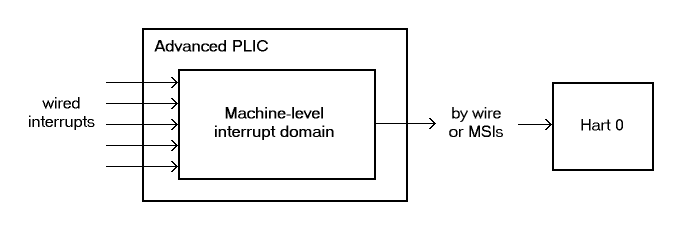
\includegraphics[scale=0.55]{AdvPLIC-ex-1Domain.png}}
\caption{%
Example of a {\RISCV} system that has a single hart implementing only
\mbox{M-mode}, with a single machine-level interrupt domain for that
hart.%
}
\label{fig:AdvPLIC-ex-1Domain}
\end{figure}

\begin{figure}[th]
\centerline{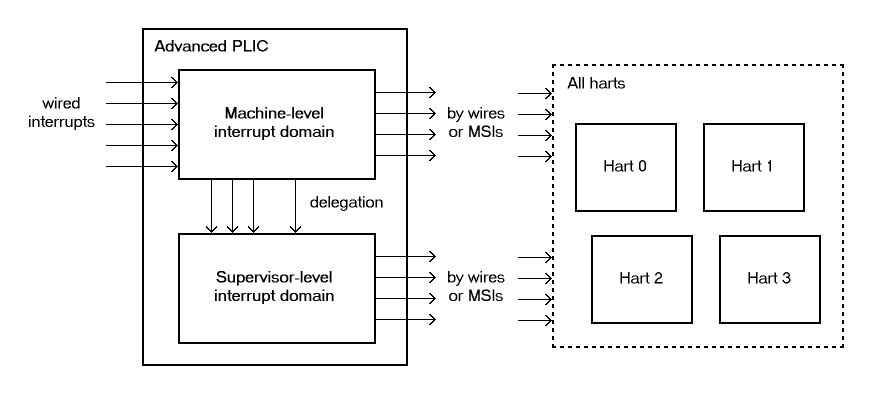
\includegraphics[scale=0.55]{AdvPLIC-ex-2Domains.png}}
\caption{%
An example system with four harts that implement \mbox{M-mode} and
\mbox{S-mode}, with two APLIC interrupt domains, one each for machine
and supervisor levels.%
}
\label{fig:AdvPLIC-ex-2Domains}
\end{figure}

An APLIC's interrupt domains are arranged in a tree hierarchy, with the
root domain always being at machine level.
Incoming interrupt wires arrive first at the root domain.
Each domain may then selectively delegate all or a subset of interrupt
sources to its child domains in the hierarchy.
Within a given APLIC, interrupt source numbers are invariant across all
domains, so source identity number~$i$ always refers to the same source
in every domain, corresponding to incoming wire number~$i$.
For an interrupt domain below the root, interrupt sources not delegated
down to that domain appear to the domain as being not implemented.

Figure~\ref{fig:AdvPLIC-ex-3Domains} shows a hierarchy of three
interrupt domains, two at machine level and one at supervisor level.
The arrangement in the figure, when combined with PMP (physical memory
protection), allows machine-level software to isolate a selection
of interrupts exclusively for hart~0, beyond the reach of the four
application harts, even at machine level.

\begin{figure}[th]
\centerline{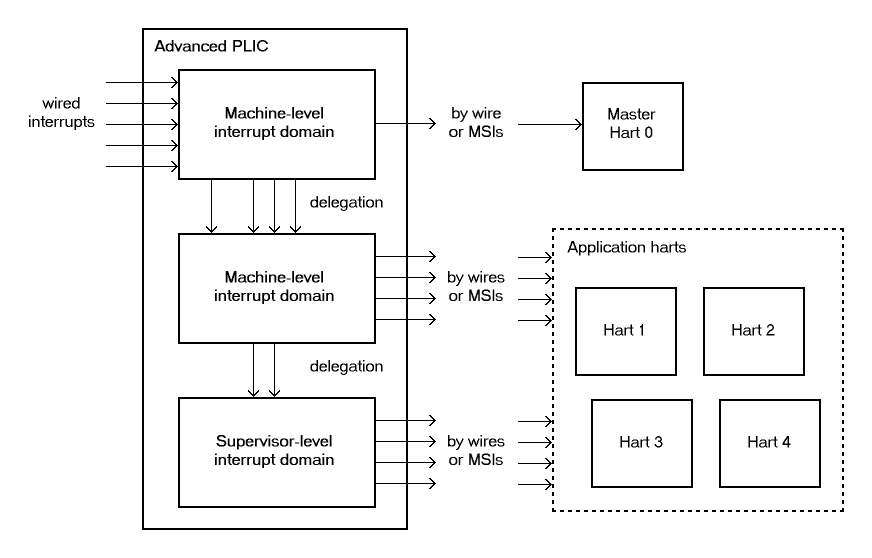
\includegraphics[scale=0.55]{AdvPLIC-ex-3Domains.png}}
\caption{%
A {\RISCV} system that extends the example of
Figure~\ref{fig:AdvPLIC-ex-2Domains} with a fifth \mbox{M-mode}-only
``manager'' hart, with a separate machine-level interrupt domain above
the other domains.%
}
\label{fig:AdvPLIC-ex-3Domains}
\end{figure}

%*** REMOVE?:
\FloatBarrier

\begin{commentary}
In order for the harts within an interrupt domain to have direct
control over the interrupts from the domain, the harts must be
cooperatively controlled by software at the same privilege level.
In particular, a single operating system should control all of the
harts associated with a supervisor-level interrupt domain.
In the examples of Figures \ref{fig:AdvPLIC-ex-2Domains}
and~\ref{fig:AdvPLIC-ex-3Domains}, control of the APLIC's
supervisor-level interrupt domain could not be safely split among
multiple independent OSes.

Given the domain hierarchies depicted in the figures, if it were
necessary to partition the application harts for multiple OSes,
machine-level software would need to prevent direct OS access to the
supervisor-level interrupt domain and instead provide SBI services
for controlling APLIC interrupts or, alternatively, emulate the control
interfaces of separate supervisor-level interrupt domains, one for each
OS.
Note that such emulation might still make use of the APLIC's
physical supervisor-level interrupt domain, but under the control of
machine-level software.
\end{commentary}

An APLIC's interrupt domain hierarchy satisfies these rules:
\begin{itemize}

\item
The root domain is at machine level.

\item
The parent of any supervisor-level interrupt domain is a machine-level
domain that includes at least the same harts (but at machine level,
obviously).
The parent domain may have a larger set of harts at machine level.

\item
For each interrupt domain, interrupts from the domain are signaled
to harts all by the same method, either by wire or by MSIs, not by a
mixture of methods among the harts.

\end{itemize}

When a {\RISCV} hart's external interrupt controller is an APLIC, not an
IMSIC, the hart can be within only one interrupt domain of this APLIC at
each privilege level.

On the other hand, a hart that has an IMSIC for its external interrupt
controller may, at each privilege level, be in multiple APLIC interrupt
domains, even those of the same APLIC, and may potentially receive MSIs
from multiple different APLICs in the machine.

A platform might give software a way to choose between multiple
interrupt domain hierarchies for any given APLIC.
Any such configurability is outside the scope of this specification,
but should be available to machine level only.

%-----------------------------------------------------------------------
\section{Hart index numbers}

Within a given interrupt domain, each of the domain's harts has a
unique \emph{index number} in the range 0 to ${\mbox{2}^{14}-\mbox{1}}$
(=~16,383).
The index number a domain associates with a hart may or may not have
any relationship to the unique hart identifier (``hart ID'') that the
{\RISCV} Privileged Architecture assigns to the hart.
Two different interrupt domains may employ entirely different index
numbers for the same set of harts.
However, if any of an APLIC's interrupt domains can forward interrupts by
MSI, then all machine-level domains of the APLIC share a common mapping
of index numbers to harts.

\begin{commentary}
For efficiency, implementations should prefer small integers for hart
index numbers.
\end{commentary}

%-----------------------------------------------------------------------
\section{Overview of interrupt control for a single domain}

Each interrupt domain implemented by an APLIC has its own separate
physical control interface that is memory-mapped in the machine's
address space, allowing access to each domain to be easily regulated
by both PMP (physical memory protection) and page-based address
translation.
The control interfaces of all interrupt domains have a common
structure.
In most respects, every domain appears to software as though it were
a root domain, without visibility of the domains above it in the
hierarchy.

An individual interrupt domain has the following components for each
interrupt source at the APLIC:
\begin{itemize}

\item
Source configuration.
This determines whether the specific source is active in the domain
and, if so, how the incoming wire is to be interpreted, such as
level-sensitive or edge-sensitive.
For a source that is inactive in the domain, source configuration
controls any delegation to a child domain.

\item
Interrupt-pending and interrupt-enable bits.
For an inactive source, these two bits are read-only zeros.
Otherwise, the pending bit records an interrupt that arrived and has
not yet been signaled or forwarded, while the enable bit determines
whether interrupts from this source should currently be delivered, or
should remain pending.

\item
Target selection.
For an active source, target selection determines the hart to receive
the interrupt and either the interrupt's priority or the new interrupt
identity when forwarding as an MSI.

\end{itemize}

For interrupt domains that deliver interrupts directly to harts rather
than forwarding by MSIs, the domain has a final set of components for
controlling interrupt delivery to harts, one instance per hart in the
domain.

\begin{commentary}
Although an APLIC with multiple interrupt domains may appear to duplicate
the per-source state listed above (source configuration, etc.)\ by a
factor equal to the number of domains, in fact, APLIC implementations
can exploit the fact that each source is ultimately active in only one
domain.
In all domains to which a specific interrupt source has not been
delegated, the state associated with the source appears as read-only
zeros, requiring no physical register bits.
\end{commentary}

%-----------------------------------------------------------------------
\section{Memory-mapped control region for an interrupt domain}
\label{sec:AdvPLIC-domainControlRegion}

For each interrupt domain that an APLIC supports, there is a dedicated
memory-mapped control region for managing interrupts in that domain.
This control region is a multiple of 4~KiB in size and aligned to a
\mbox{4-KiB} address boundary.
The smallest valid control region is 16~KiB.
An interrupt domain's control region is populated by a set of
\mbox{32-bit} registers.
The first 16~KiB contains the registers listed in
Table~\ref{tab:AdvPLIC-domainControlRegion}.

\begin{table*}[p]
\begin{center}
\begin{tabular}{c@{\quad\ }l@{\qquad}ll}
\multicolumn{1}{l}{offset} & \ size & register name \\
\noalign{\medskip}
\z{0x0000} & 4 bytes & \z{domaincfg} \\
\z{0x0004} & 4 bytes & \z{sourcecfg[}1\z{]} \\
\z{0x0008} & 4 bytes & \z{sourcecfg[}2\z{]} \\
\dots      &         & \ \dots \\
\z{0x0FFC} & 4 bytes & \z{sourcecfg[}1023\z{]} \\
\z{0x1BC0} & 4 bytes & \z{mmsiaddrcfg}  & (machine-level interrupt domains only) \\
\z{0x1BC4} & 4 bytes & \z{mmsiaddrcfgh} & \quad '' \\
\z{0x1BC8} & 4 bytes & \z{smsiaddrcfg}  & \quad '' \\
\z{0x1BCC} & 4 bytes & \z{smsiaddrcfgh} & \quad '' \\
\z{0x1C00} & 4 bytes & \z{setip[}0\z{]} \\
\z{0x1C04} & 4 bytes & \z{setip[}1\z{]} \\
\dots      &         & \ \dots \\
\z{0x1C7C} & 4 bytes & \z{setip[}31\z{]} \\
\z{0x1CDC} & 4 bytes & \z{setipnum} \\
\z{0x1D00} & 4 bytes & \z{in\_clrip[}0\z{]} \\
\z{0x1D04} & 4 bytes & \z{in\_clrip[}1\z{]} \\
\dots      &         & \ \dots \\
\z{0x1D7C} & 4 bytes & \z{in\_clrip[}31\z{]} \\
\z{0x1DDC} & 4 bytes & \z{clripnum} \\
\z{0x1E00} & 4 bytes & \z{setie[}0\z{]} \\
\z{0x1E04} & 4 bytes & \z{setie[}1\z{]} \\
\dots      &         & \ \dots \\
\z{0x1E7C} & 4 bytes & \z{setie[}31\z{]} \\
\z{0x1EDC} & 4 bytes & \z{setienum} \\
\z{0x1F00} & 4 bytes & \z{clrie[}0\z{]} \\
\z{0x1F04} & 4 bytes & \z{clrie[}1\z{]} \\
\dots      &         & \ \dots \\
\z{0x1F7C} & 4 bytes & \z{clrie[}31\z{]} \\
\z{0x1FDC} & 4 bytes & \z{clrienum} \\
\z{0x2000} & 4 bytes & \z{setipnum\_le} \\
\z{0x2004} & 4 bytes & \z{setipnum\_be} \\
\z{0x3000} & 4 bytes & \z{genmsi} \\
\z{0x3004} & 4 bytes & \z{target[}1\z{]} \\
\z{0x3008} & 4 bytes & \z{target[}2\z{]} \\
\dots      &         & \ \dots \\
\z{0x3FFC} & 4 bytes & \z{target[}1023\z{]} \\
\end{tabular}
\end{center}
\bigskip
\caption{%
The registers of the first 16~KiB of an interrupt domain's memory-mapped
control region.%
}
\label{tab:AdvPLIC-domainControlRegion}
\end{table*}

Starting at offset \z{0x4000}, an interrupt domain's control region
may optionally have an array of \emph{interrupt delivery control} (IDC)
structures, one for each potential hart index number in the range 0 to
some maximum that is at least as large as the maximum hart index number
for the interrupt domain.
IDC structures are used only when the domain is configured to deliver
interrupts directly to harts instead of being forwarded by MSIs.
An interrupt domain that supports only interrupt forwarding by MSIs
and not the direct delivery of interrupts by the APLIC does not need IDC
structures in its control region.

The first IDC structure, if any, is for the hart with index number~0;
the second is for the hart with index number~1; and so forth.
Each IDC structure is 32~bytes and has these defined registers:
\begin{displayLinesTable}[c@{\quad\ }l@{\qquad}l]
offset   & \ size  & register name \\
\noalign{\medskip}
\z{0x00} & 4 bytes & \z{idelivery} \\
\z{0x04} & 4 bytes & \z{iforce} \\
\z{0x08} & 4 bytes & \z{ithreshold} \\
\z{0x18} & 4 bytes & \z{topi} \\
\z{0x1C} & 4 bytes & \z{claimi} \\
\end{displayLinesTable}
IDC structures are packed contiguously, 32~bytes per structure, so the
offset from the beginning of an interrupt domain's control region to
its second IDC structure (hart index~1), if it exists, is \z{0x4020};
the offset to the third IDC structure (hart index~2), if it exists, is
\z{0x4040}; etc.

The array of IDC structures may include some for \emph{potential} hart
index numbers that are not \emph{actual} hart index numbers in the
domain.
For example, the first IDC structure is always for hart index~0, but 0
is not necessarily a valid index number for any hart in the domain.
For each IDC structure in the array that does not correspond to a valid
hart index number in the domain, the IDC structure's registers may
(or may not) be all read-only zeros.

Aside from the registers in Table~\ref{tab:AdvPLIC-domainControlRegion}
and those listed above for IDC structures, all other bytes in an
interrupt domain's control region are reserved and are implemented as
read-only zeros.

Only naturally aligned \mbox{32-bit} simple reads and writes are
supported within an interrupt domain's control region.
Writes to read-only bytes are ignored.
For other forms of accesses (other sizes, misaligned accesses, or
AMOs), implementations should preferably report an access fault or
bus error but must otherwise ignore the access.

The registers of the first 16~KiB of an interrupt domain's control
region (all but the IDC structures) are documented individually below.
IDC structures are documented later, in
Section~\ref{sec:AdvPLIC-directMode},
``Interrupt delivery directly by the APLIC.''

%- - - - - - - - - - - - - - - - - - - - - - - - - - - - - - - - - - - -
\subsection{Domain configuration (\zSafe{domaincfg})}
\label{sec:AdvPLIC-reg-domaincfg}

The \z{domaincfg} register has this format:\nopagebreak
\begin{displayLinesTable}[l@{\quad}l]
bits 31:24 & read-only \z{0x80} \\
bit 8      & IE \\
bit 7      & read-only 0 \\
bit 2      & DM (\WARL) \\
bit 0      & BE (\WARL) \\
\end{displayLinesTable}
All other register bits are reserved and read as zeros.

Bit IE (Interrupt Enable) is a global enable for all active interrupt
sources at this interrupt domain.
Only when IE~=~1 are pending-and-enabled interrupts actually signaled
or forwarded to harts.

Field DM (Delivery Mode) is {\WARL} and determines how this interrupt
domain delivers interrupts to harts.
The two possible values for DM are:
\begin{displayLinesTable}
0~=~direct delivery mode\\
1~=~MSI delivery mode\\
\end{displayLinesTable}
In \emph{direct delivery mode}, interrupts are prioritized and signaled
directly to harts by the APLIC itself.
In \emph{MSI delivery mode}, interrupts are forwarded by the APLIC
as MSIs to harts, presumably for further handling by IMSICs at those
harts.
A given APLIC implementation may support either or both of these
delivery modes for each interrupt domain.

If the interrupt domain's harts have IMSICs,
then unless the relevant interrupt
files of those IMSICs support value \z{0x40000000} for register
\z{eidelivery}, setting DM to zero (direct delivery mode) will
have the same effect as setting IE to zero.
See Sections \ref{sec:IMSIC-reg-eidelivery}
and~\ref{sec:AdvPLIC-directMode-intrDelivery}.

BE (Big-Endian) is a {\WARL} field that determines the byte order for
most registers in the interrupt domain's memory-mapped control region.
If BE~=~0, byte order is little-endian, and if BE~=~1, it is
big-endian.
For {\RISCV} systems that support only little-endian, BE may be
read-only zero, and for those that support only big-endian, BE may be
read-only one.
For bi-endian systems, BE is writable.

Field BE affects the byte order of accesses to the \z{domaincfg}
register itself, just as for other registers in the interrupt domain's
control region.
To deal with this fact, the read-only value in \z{domaincfg}'s
most-significant byte, bits 31:24, serves two purposes.
First, for any read of \z{domaincfg}, the register's correct byte order
is easily determined from the four-byte value obtained:
When interpreted in the correct byte order, bit~31 is one, and in the
wrong order, bit~31 is zero.
Second, if the value of BE is uncertain (prior to software
initializing the interrupt domain, presumably), an \mbox{8-bit}
value~$x$ can be safely written to \z{domaincfg} by writing
\mbox{($x$\,\z{<<}\,24) \z{|} $x$}, where \mbox{\z{<<}\,24} represents
shifting left by 24~bits, and the vertical bar (\z{|}) represents
bitwise logical OR.
After \z{domaincfg} is written once, the value of BE should then be
known, so subsequent writes should not need to repeat the same trick.

At system reset, all writable bits in \z{domaincfg} are initialized to
zero, including~IE.
If an implementation supports additional forms of reset for the APLIC,
it is implementation-defined (or possibly platform-defined) how these
other resets may affect \z{domaincfg}.

%- - - - - - - - - - - - - - - - - - - - - - - - - - - - - - - - - - - -
\subsection{%
Source configurations
 (\zSafe{sourcecfg[{\rm 1}]}--\zSafe{sourcecfg[{\rm 1023}]})%
}
\label{sec:AdvPLIC-reg-sourcecfg}

For each possible interrupt source~$i$, register \z{sourcecfg[$i$]}
controls the \emph{source mode} for source~$i$ in this interrupt domain
as well as any delegation of the source to a child domain.
When source~$i$ is not implemented, or appears in this domain not to be
implemented, \z{sourcecfg[$i$]} is read-only zero.
If source~$i$ was not delegated to this domain and is then
changed (at the parent domain) to become delegated to this domain,
\z{sourcecfg[$i$]} remains zero until successfully written with a
nonzero value.

Bit~10 of \z{sourcecfg[$i$]} is a \mbox{1-bit} field called~D
(Delegate).
If D~=~1, source~$i$ is delegated to a child domain, and if D~=~0, it
is not delegated to a child domain.
Interpretation of the rest of \z{sourcecfg[$i$]} depends on field~D.

When interrupt source~$i$ is delegated to a child domain,
\z{sourcecfg[$i$]} has this format:\nopagebreak
\begin{displayLinesTable}[l@{\qquad}l]
bit 10   & D, = 1 \\
bits 9:0 & Child Index (\WLRL) \\
\end{displayLinesTable}
All other register bits are reserved and read as zeros.

Child Index is a {\WLRL} field that specifies the interrupt domain to
which this source is delegated.
For an interrupt domain with $C$~child domains, this field must be able
to hold integer values in the range 0 to ${C-\mbox{1}}$.
Each interrupt domain has a fixed mapping from these index numbers to
child domains.

If an interrupt domain has no children in the domain hierarchy, bit~D
cannot be set to one in any \z{sourcecfg} register for that domain.
For such a leaf domain, attempting to write a \z{sourcecfg} register
with a value that has bit~10 =~1 causes the entire register to be set
to zero instead.

When interrupt source~$i$ is not delegated to a child domain,
\z{sourcecfg[$i$]} has this format:\nopagebreak
\begin{displayLinesTable}[l@{\qquad}l]
bit 10   & D, = 0 \\
bits 2:0 & SM (\WARL) \\
\end{displayLinesTable}
All other register bits are reserved and read as zeros.

The SM (Source Mode) field is {\WARL} and controls whether the
interrupt source is active in this domain, and if so, what values or
transitions on the incoming wire are interpreted as interrupts.
The values allowed for SM and their meanings are listed in
Table~\ref{tab:AdvPLIC-sourcecfg-SM}.
Inactive (zero) is always supported for field~SM.
Implementations are free to choose, independently for each interrupt
source, what other values are supported for SM.

\begin{table*}[h!]
\begin{center}
\begin{tabular}{|c|c|l|}
\hline
Value & Name   & Description \\
\hline
\hline
0    & Inactive & Inactive in this domain (and not delegated) \\
1    & Detached & Active, detached from the source wire \\
2--3 & ---      & \emph{Reserved} \\
4    & Edge1    & Active, edge-sensitive; interrupt asserted on rising edge \\
5    & Edge0    & Active, edge-sensitive; interrupt asserted on falling edge \\
6    & Level1   & Active, level-sensitive; interrupt asserted when high \\
7    & Level0   & Active, level-sensitive; interrupt asserted when low \\
\hline
\end{tabular}
\end{center}
\caption{%
Encoding of the SM (Source Mode) field of a \z{sourcecfg} register when
bit~D =~0%
}
\label{tab:AdvPLIC-sourcecfg-SM}
\end{table*}

An interrupt source is inactive in the interrupt domain if either the
source is delegated to a child domain (D~=~1) or it is not delegated
(D~=~0) and SM is Inactive.
Whenever interrupt source~$i$ is inactive in an interrupt domain,
the corresponding interrupt-pending and interrupt-enable bits within
the domain are read-only zeros, and register \z{target[$i$]} is also
read-only zero.
If source~$i$ is changed from inactive to an active mode, the
interrupt source's pending and enable bits remain zeros, unless set
automatically for a reason specified later in this section or in
Section~\ref{sec:AdvPLIC-pendingBits}, and the defined subfields
of \z{target[$i$]} obtain {\unspecified} values.

When a source is configured as Detached, its wire input is ignored;
however, the interrupt-pending bit may still be set by a write to a
\z{setip} or \z{setipnum} register.
(This mode can be useful for receiving MSIs, for example.)

An edge-sensitive source can be configured to recognize an incoming
interrupt on either a rising edge (low-to-high transition) or a falling
edge (high-to-low transition).
When configured for a falling edge (mode Edge0), the source is said to
be \emph{inverted}.

A level-sensitive source can be configured to interpret either a
high level~(1) or a low level~(0) on the wire as the assertion of an
interrupt.
When configured for a low level (mode Level0), the source is said to be
\emph{inverted}.

For an interrupt source that is configured as edge-sensitive or
level-sensitive, define\nopagebreak
\begin{displayLinesTable}
\emph{rectified input value} = (incoming wire value) XOR (source is inverted).
\end{displayLinesTable}
For a source that is inactive or Detached, the
\emph{rectified input value} is zero.

Any write to a \z{sourcecfg} register might (or might not) cause the
corresponding interrupt-pending bit to be set to one if the rectified
input value is high (=~1) under the new source mode.
A write to a \z{sourcecfg} register will not by itself cause a pending
bit to be cleared except when the source is made inactive.
(But see Section~\ref{sec:AdvPLIC-pendingBits}.)

%- - - - - - - - - - - - - - - - - - - - - - - - - - - - - - - - - - - -
\subsection{%
Machine MSI address configuration
 (\zSafe{mmsiaddrcfg} and \zSafe{mmsiaddrcfgh})%
}
\label{sec:AdvPLIC-reg-mmsiaddrcfg}

For machine-level interrupt domains, registers \z{mmsiaddrcfg}
and \z{mmsiaddrcfgh} may optionally provide parameters used to
determine the addresses to write outgoing MSIs.

If no interrupt domain of the APLIC supports MSI delivery
mode (\z{domaincfg}.DM is read-only zero for all domains),
these two registers are not implemented for any domain.
Otherwise, they are implemented for the root domain, and may
or may not be implemented for other machine-level domains.
For domains not at machine level, they are never implemented.
When a domain does not implement \z{mmsiaddrcfg} and
\z{mmsiaddrcfgh}, the eight bytes at their locations
are simply read-only zeros like other reserved bytes.

Registers \z{mmsiaddrcfg} and \z{mmsiaddrcfgh} are
potentially writable only for the root domain.
For all other machine-level domains that implement them,
they are read-only.

When implemented, \z{mmsiaddrcfg} has this format:\nopagebreak
\begin{displayLinesTable}[l@{\quad}l]
bits 31:0 & Low Base PPN (\WARL) \\
\end{displayLinesTable}
and \z{mmsiaddrcfgh} has this format:\nopagebreak
\begin{displayLinesTable}[l@{\quad}l]
bit 31     & L \\
bits 28:24 & HHXS (\WARL) \\
bits 22:20 & LHXS (\WARL) \\
bits 18:16 & HHXW (\WARL) \\
bits 15:12 & LHXW (\WARL) \\
bits 11:0  & High Base PPN (\WARL) \\
\end{displayLinesTable}
All other bits of \z{mmsiaddrcfgh} are reserved and read as zeros.

Fields High Base PPN from \z{mmsiaddrcfgh} and Low Base PPN from
\z{mmsiaddrcfg} concatenate to form a \mbox{44-bit} Base PPN
(Physical Page Number).
The use of this value and fields HHXS (High Hart Index Shift),
LHXS (Low Hart Index Shift), HHXW (High Hart Index Width),
and LHXW (Low Hart Index Width) for
determining target addresses for MSIs is described later, in
Section~\ref{sec:AdvPLIC-MSIAddrs}.

When \z{mmsiaddrcfg} and \z{mmsiaddrcfgh} are writable
(root domain only), all fields other than L are {\WARL}.
An implementation is free to choose what values are supported.
Typically, some bits are writable while others are read-only constants.
In the extreme, the values of all fields may be entirely
constant, fixed by the implementation.

If bit~L in \z{mmsiaddrcfgh} is set to one, \z{mmsiaddrcfg} and
\z{mmsiaddrcfgh} are \emph{locked}, and writes to the registers are
ignored, making the registers effectively read-only.
When L~=~1, the other fields in \z{mmsiaddrcfg} and \z{mmsiaddrcfgh}
may optionally all read as zeros.
In that case, if these other fields were given nonzero values
when L was first set in the root domain,
their values are retained internally by the
APLIC but become no longer visible by reading \z{mmsiaddrcfg} and
\z{mmsiaddrcfgh}.

Setting \z{mmsiaddrcfgh}.L to one also locks registers
\z{smsiaddrcfg} and \z{smsiaddrcfgh} described in the next
subsection, if those registers are implemented as well.

For the root domain, L~is initialized at
system reset to either zero or one, whichever is
deemed appropriate for the specific APLIC implementation.
If reset initializes L to one, either the other fields are
hardwired by the APLIC to constants, or the APLIC has a different means,
outside of this standard, for determining the addresses of outgoing MSI
writes.
In the latter case, the other fields in \z{mmsiaddrcfg} and
\z{mmsiaddrcfgh} may all read as zeros, so registers \z{mmsiaddrcfg} and
\z{mmsiaddrcfgh} have only read-only values zero and \z{0x80000000}
respectively.
Any time \z{mmsiaddrcfg} or \z{mmsiaddrcfgh} has a different value
(not zero or \z{0x80000000} respectively), the addresses for
outgoing MSI writes directed to machine level must be derivable
from the visible values of these registers, as specified in
Section~\ref{sec:AdvPLIC-MSIAddrs}.

For machine-level domains that are not the root domain, if these
registers are implemented, bit~L is always one, and the other
fields either are read-only copies of \z{mmsiaddrcfg} and
\z{mmsiaddrcfgh} from the root domain, or are all zeros.

\begin{commentary}
Giving software the ability to arbitrarily determine the addresses to
which MSIs are sent, even if allowed only for machine level, permits
bypassing physical memory protection (PMP).
For APLICs that support MSI delivery mode, it is recommended, if
feasible, that the APLIC internally hardwire the physical addresses for
all target IMSICs, putting those addresses beyond the reach of software
to change.
However, not all APLIC implementations will be able to follow that
recommendation.

It is expected that most systems will arrange the
physical addresses of target IMSICs in a simple
linear correspondence with hart index numbers.
(See Section~\ref{sec:IMSIC-systemMemRegions}.)
Registers \z{mmsiaddrcfg} and \z{mmsiaddrcfgh} (along with
\z{smsiaddrcfg} and \z{smsiaddrcfgh} from the next subsection) allow
sufficiently trusted machine-level software, early after system reset,
to configure the pattern of physical addresses for target IMSICs and
then lock this configuration against subsequent tampering.

APLICs that actually hardwire the IMSIC addresses internally
can implement these registers simply as read-only with values zero
and \z{0x80000000}.
Or, if the IMSIC addresses must be configured by software but
the formula is too complex for registers \z{mmsiaddrcfg} and
\z{mmsiaddrcfgh} to handle, again the registers can be implemented
simply as read-only with values zero and \z{0x80000000}, and a
separate, custom mechanism supplied for configuring the IMSIC
addresses.
\end{commentary}

If an APLIC supports additional forms of reset
besides system reset, it is implementation-defined (or possibly
platform-defined) how these other resets may affect \z{mmsiaddrcfg} and
\z{mmsiaddrcfgh} (as well as \z{smsiaddrcfg} and \z{smsiaddrcfgh})
in the root domain.
However, it must not be possible for insufficiently privileged software
to use a localized reset to unlock these registers by changing bit~L
back to zero.
For this reason, it is likely that only a complete system reset affects
these registers, and any other resets do not.

%- - - - - - - - - - - - - - - - - - - - - - - - - - - - - - - - - - - -
\subsection{%
Supervisor MSI address configuration
 (\zSafe{smsiaddrcfg} and \zSafe{smsiaddrcfgh})%
}
\label{sec:AdvPLIC-reg-smsiaddrcfg}

For machine-level interrupt domains, registers \z{smsiaddrcfg} and
\z{smsiaddrcfgh} may optionally provide parameters used by
supervisor-level domains to determine the addresses to write outgoing
MSIs.

Registers \z{smsiaddrcfg} and \z{smsiaddrcfgh} are implemented
by a domain if the domain implements \z{mmsiaddrcfg} and
\z{mmsiaddrcfgh} and the APLIC has at least one supervisor-level
interrupt domain.
If the registers are not implemented, the eight bytes at their
locations are simply read-only zeros like other reserved bytes.

Like \z{mmsiaddrcfg} and \z{mmsiaddrcfgh}, registers
\z{smsiaddrcfg} and \z{smsiaddrcfgh} are potentially
writable only for the root domain.
For all other machine-level domains that implement them,
they are read-only.

When implemented, \z{smsiaddrcfg} has this format:\nopagebreak
\begin{displayLinesTable}[l@{\quad}l]
bits 31:0 & Low Base PPN (\WARL) \\
\end{displayLinesTable}
and \z{smsiaddrcfgh} has this format:\nopagebreak
\begin{displayLinesTable}[l@{\quad}l]
bits 22:20 & LHXS (\WARL) \\
bits 11:0  & High Base PPN (\WARL) \\
\end{displayLinesTable}
All other bits of \z{smsiaddrcfgh} are reserved and read as zeros.

Fields High Base PPN from \z{smsiaddrcfgh} and Low Base PPN from
\z{smsiaddrcfg} concatenate to form a \mbox{44-bit} Base PPN
(Physical Page Number).
The use of this value and field LHXS (Low Hart Index Shift) for
determining target addresses for MSIs is described later, in
Section~\ref{sec:AdvPLIC-MSIAddrs}.

When \z{smsiaddrcfg} and \z{smsiaddrcfgh} are writable
(root domain only), all fields are {\WARL}.
An implementation is free to choose what values are supported, just as
for \z{mmsiaddrcfg} and \z{mmsiaddrcfgh}.

If register \z{mmsiaddrcfgh} of the domain has bit~L set to one,
then \z{smsiaddrcfg} and \z{smsiaddrcfgh} are \emph{locked}
as read-only alongside \z{mmsiaddrcfg} and \z{mmsiaddrcfgh}.
When \z{mmsiaddrcfgh}.L~=~1, if the readable values of \z{mmsiaddrcfg}
and \z{mmsiaddrcfgh} are zero and \z{0x80000000} respectively---because
their other fields are hidden---then \z{smsiaddrcfg} and
\z{smsiaddrcfgh} are hidden also and read as zeros.

For the root domain only, if \z{mmsiaddrcfgh}.L =~1 and the
MSI-address-configuration fields are hidden (so \z{mmsiaddrcfgh}
reads as \z{0x80000000} and registers \z{mmsiaddrcfg},
\z{smsiaddrcfg}, and \z{smsiaddrcfgh} all read as zeros),
then whatever values \z{smsiaddrcfg} and \z{smsiaddrcfgh} had when
\z{mmsiaddrcfgh}.L was first set are retained internally by the APLIC,
though those values are no longer visible by reading the registers.
Alternatively, if system reset initializes \z{mmsiaddrcfgh}.L =~1 in
the root domain, and if all MSI-address-configuration fields never
appear as anything other than zeros, then the APLIC implementation
has some other, possibly nonstandard, means for determining
the addresses of outgoing MSIs, as discussed in the previous
subsection, \ref{sec:AdvPLIC-reg-mmsiaddrcfg}.

Any time \z{mmsiaddrcfg} and \z{mmsiaddrcfgh} are not read-only
zero and \z{0x80000000} respectively, the addresses for outgoing
MSI writes directed to supervisor level must be derivable from the
visible values of registers \z{mmsiaddrcfgh}, \z{smsiaddrcfg}, and
\z{smsiaddrcfgh}, as specified in Section~\ref{sec:AdvPLIC-MSIAddrs}.

For machine-level domains that are not the root domain,
if \z{smsiaddrcfg} and \z{smsiaddrcfgh} are implemented
and are not read-only zeros, then they are read-only
copies of the same registers from the root domain.

%- - - - - - - - - - - - - - - - - - - - - - - - - - - - - - - - - - - -
\subsection{%
Set interrupt-pending bits (\zSafe{setip[{\rm 0}]}--\zSafe{setip[{\rm 31}]})%
}

Reading or writing register \z{setip[$k$]} reads or potentially
modifies the pending bits for interrupt sources $k\times\mbox{32}$
through ${k\times\mbox{32}+\mbox{31}}$.
For an implemented interrupt source~$i$ within that range, the pending
bit for source~$i$ corresponds with register bit ${(i\bmod\mbox{32})}$.

A read of a \z{setip} register returns the pending bits of the
corresponding interrupt sources.
Bit positions in the result value that do not correspond to an
implemented interrupt source (such as bit~0 of \z{setip[{\rm 0}]}) are
zeros.

On a write to a \z{setip} register, for each bit that is one in the
\mbox{32-bit} value written, if that bit position corresponds to an
active interrupt source, the interrupt-pending bit for that source is
set to one if possible.
See Section~\ref{sec:AdvPLIC-pendingBits} for exactly when a pending
bit may be set by writing to a \z{setip} register.

%- - - - - - - - - - - - - - - - - - - - - - - - - - - - - - - - - - - -
\subsection{Set interrupt-pending bit by number (\zSafe{setipnum})}

If $i$ is an active interrupt source number in the domain, writing
\mbox{32-bit} value~$i$ to register \z{setipnum} causes the pending bit
for source~$i$ to be set to one if possible.
See Section~\ref{sec:AdvPLIC-pendingBits} for exactly when a pending
bit may be set by writing to \z{setipnum}.

A write to \z{setipnum} is ignored if the value written is not an
active interrupt source number in the domain.
A read of \z{setipnum} always returns zero.

%- - - - - - - - - - - - - - - - - - - - - - - - - - - - - - - - - - - -
\subsection{%
Rectified inputs, clear interrupt-pending bits
 (\zSafe{in\_clrip[{\rm 0}]}--\zSafe{in\_clrip[{\rm 31}]})%
}

Reading register \z{in\_clrip[$k$]} returns the rectified input
values (Section~\ref{sec:AdvPLIC-reg-sourcecfg}) for interrupt sources
$k\times\mbox{32}$ through ${k\times\mbox{32}+\mbox{31}}$, while
writing \z{in\_clrip[$k$]} potentially modifies the pending bits for
the same sources.
For an implemented interrupt source~$i$ within the specified range,
source~$i$ corresponds with register bit ${(i\bmod\mbox{32})}$.

A read of an \z{in\_clrip} register returns the rectified input values
of the corresponding interrupt sources.
Bit positions in the result value that do not correspond to an
implemented interrupt source (such as bit~0 of \z{in\_clrip[{\rm 0}]})
are zeros.

On a write to an \z{in\_clrip} register, for each bit that is one in
the \mbox{32-bit} value written, if that bit position corresponds to an
active interrupt source, the interrupt-pending bit for that source is
cleared if possible.
See Section~\ref{sec:AdvPLIC-pendingBits} for exactly when a pending
bit may be cleared by writing to an \z{in\_clrip} register.

%- - - - - - - - - - - - - - - - - - - - - - - - - - - - - - - - - - - -
\subsection{Clear interrupt-pending bit by number (\zSafe{clripnum})}

If $i$ is an active interrupt source number in the domain, writing
\mbox{32-bit} value~$i$ to register \z{clripnum} causes the pending bit
for source~$i$ to be cleared if possible.
See Section~\ref{sec:AdvPLIC-pendingBits} for exactly when a pending
bit may be cleared by writing to \z{clripnum}.

A write to \z{clripnum} is ignored if the value written is not an
active interrupt source number in the domain.
A read of \z{clripnum} always returns zero.

%- - - - - - - - - - - - - - - - - - - - - - - - - - - - - - - - - - - -
\subsection{%
Set interrupt-enable bits (\zSafe{setie[{\rm 0}]}--\zSafe{setie[{\rm 31}]})%
}

Reading or writing register \z{setie[$k$]} reads or potentially
modifies the enable bits for interrupt sources $k\times\mbox{32}$
through ${k\times\mbox{32}+\mbox{31}}$.
For an implemented interrupt source~$i$ within that range, the enable
bit for source~$i$ corresponds with register bit ${(i\bmod\mbox{32})}$.

A read of a \z{setie} register returns the enable bits of the
corresponding interrupt sources.
Bit positions in the result value that do not correspond to an
implemented interrupt source (such as bit~0 of \z{setie[{\rm 0}]}) are
zeros.

On a write to a \z{setie} register, for each bit that is one in the
\mbox{32-bit} value written, if that bit position corresponds to an
active interrupt source, the interrupt-enable bit for that source is
set to one.

%- - - - - - - - - - - - - - - - - - - - - - - - - - - - - - - - - - - -
\subsection{Set interrupt-enable bit by number (\zSafe{setienum})}

If $i$ is an active interrupt source number in the domain, writing
\mbox{32-bit} value~$i$ to register \z{setienum} causes the enable bit
for source~$i$ to be set to one.

A write to \z{setienum} is ignored if the value written is not an
active interrupt source number in the domain.
A read of \z{setienum} always returns zero.

%- - - - - - - - - - - - - - - - - - - - - - - - - - - - - - - - - - - -
\subsection{%
Clear interrupt-enable bits (\zSafe{clrie[{\rm 0}]}--\zSafe{clrie[{\rm 31}]})%
}

Writing register \z{clrie[$k$]} potentially modifies the
enable bits for interrupt sources $k\times\mbox{32}$ through
${k\times\mbox{32}+\mbox{31}}$.
For an implemented interrupt source~$i$ within that range, the enable
bit for source~$i$ corresponds with register bit ${(i\bmod\mbox{32})}$.

On a write to a \z{clrie} register, for each bit that is one in the
\mbox{32-bit} value written, the interrupt-enable bit for that source
is cleared.

A read of a \z{clrie} register always returns zero.

%- - - - - - - - - - - - - - - - - - - - - - - - - - - - - - - - - - - -
\subsection{Clear interrupt-enable bit by number (\zSafe{clrienum})}

If $i$ is an active interrupt source number in the domain, writing
\mbox{32-bit} value~$i$ to register \z{clrienum} causes the enable bit
for source~$i$ to be cleared.

A write to \z{clrienum} is ignored if the value written is not an
active interrupt source number in the domain.
A read of \z{clrienum} always returns zero.

%- - - - - - - - - - - - - - - - - - - - - - - - - - - - - - - - - - - -
\subsection{%
Set interrupt-pending bit by number, little-endian (\zSafe{setipnum\_le})%
}

Register \z{setipnum\_le} acts identically to \z{setipnum} except that
byte order is always little-endian, as though field BE (Big-Endian) of
register \z{domaincfg} is zero.

For systems that are big-endian-only, with \z{domaincfg}.BE hardwired
to one, \z{setipnum\_le} need not be implemented, in which case
the four bytes at this offset are simply read-only zeros like other
reserved bytes.

\z{setipnum\_le} may be used as a write port for MSIs.

%- - - - - - - - - - - - - - - - - - - - - - - - - - - - - - - - - - - -
\subsection{%
Set interrupt-pending bit by number, big-endian (\zSafe{setipnum\_be})%
}

Register \z{setipnum\_be} acts identically to \z{setipnum} except that
byte order is always big-endian, as though field BE (Big-Endian) of
register \z{domaincfg} is one.

For systems that are little-endian-only, with \z{domaincfg}.BE
hardwired to zero, \z{setipnum\_be} need not be implemented, in which
case the four bytes at this offset are simply read-only zeros like
other reserved bytes.

For systems built mainly for big-endian byte order, \z{setipnum\_be}
may be useful as a write port for MSIs from some devices.

%- - - - - - - - - - - - - - - - - - - - - - - - - - - - - - - - - - - -
\subsection{Generate MSI (\zSafe{genmsi})}
\label{sec:AdvPLIC-reg-genmsi}

When the interrupt domain is configured in MSI delivery mode
(\z{domaincfg}.DM =~1), register \z{genmsi} can be used to cause an
\emph{extempore} MSI to be sent from the APLIC to a hart.
The main purpose for this function is to assist in establishing
a temporary known ordering between a hart's writes to the APLIC's
registers and the transmission of MSIs from the APLIC to the hart, as
explained later in Section~\ref{sec:AdvPLIC-MSISync}.

\begin{commentary}
For other purposes, sending an MSI to a hart is usually better done by
writing directly to the hart's IMSIC, rather than employing an APLIC as
an intermediary.
Use of the \z{genmsi} register should be minimized to avoid it becoming
a bottleneck.
\end{commentary}

Register \z{genmsi} has this format:\nopagebreak
\begin{displayLinesTable}[l@{\ \quad}l]
bits 31:18 & Hart Index (\WLRL) \\
bit 12     & Busy (\textbf{read-only}) \\
bits 10:0  & EIID (\WARL) \\
\end{displayLinesTable}
All other register bits are reserved and read as zeros.

The Busy bit is ordinarily zero (false), but a write to \z{genmsi}
causes Busy to become one (true), indicating an extempore MSI is
pending.
The Hart Index field specifies the destination hart, and EIID
(External Interrupt Identity) specifies the data value for the MSI.
Fields Hart Index and EIID have the same formats and behavior
as in a \z{target} register, documented in the next subsection,
\ref{sec:AdvPLIC-reg-target}.
For a machine-level interrupt domain, an extempore MSI is sent to the
destination hart at machine level, and for a supervisor-level interrupt
domain, an extempore MSI is sent to the destination hart at supervisor
level.

A pending extempore MSI should be sent by the APLIC with minimal delay.
Once it has left the APLIC and the APLIC is able to accept a new write to
\z{genmsi} for another extempore MSI, Busy reverts to false.
All MSIs previously sent from this APLIC to the same hart must be
visible at the hart's IMSIC before the extempore MSI becomes visible at
the hart's IMSIC.

While Busy is true, writes to \z{genmsi} are ignored.

Extempore MSIs are not affected by the IE bit of the domain's
\z{domaincfg} register.
An extempore MSI is sent even if \z{domaincfg}.IE~=~0.

When the interrupt domain is configured in direct delivery mode
(\z{domaincfg}.DM =~0), register \z{genmsi} is read-only zero.

%- - - - - - - - - - - - - - - - - - - - - - - - - - - - - - - - - - - -
\subsection{%
Interrupt targets (\zSafe{target[{\rm 1}]}-\zSafe{target[{\rm 1023}]})%
}
\label{sec:AdvPLIC-reg-target}

If interrupt source~$i$ is inactive in this domain, register
\z{target[$i$]} is read-only zero.
If source~$i$ is active, \z{target[$i$]} determines the hart to which
interrupts from the source are signaled or forwarded.
The exact interpretation of \z{target[$i$]} depends on the delivery
mode configured by field DM of register \z{domaincfg}.

If \z{domaincfg}.DM is changed, the \z{target} registers
for all active interrupt sources within the domain obtain
{\unspecified} values in all fields defined for the new delivery mode.

%--------------------
\subsubsection*{Active source, direct delivery mode}

For an active interrupt source~$i$, if the domain is configured
in direct delivery mode (\z{domaincfg}.DM =~0), then register
\z{target[$i$]} has this format:\nopagebreak
\begin{displayLinesTable}[l@{\ \quad}l]
bits 31:18 & Hart Index (\WLRL) \\
bits 7:0   & IPRIO (\WARL) \\
\end{displayLinesTable}
All other register bits are reserved and read as zeros.

Hart Index is a {\WLRL} field that specifies the hart to which
interrupts from this source will be delivered.

Field IPRIO (Interrupt Priority) specifies the \emph{priority number}
for the interrupt source.
This field is a {\WARL} unsigned integer of \emph{IPRIOLEN} bits, where
IPRIOLEN is a constant parameter for the given APLIC, in the range of
1 to~8.
Only values 1 through $\mbox{2}^{\textrm{IPRIOLEN}} - \mbox{1}$ are
allowed for IPRIO, not zero.
A write to a \z{target} register sets IPRIO equal to bits
$({\mbox{IPRIOLEN} - \mbox{1}})$:0 of the \mbox{32-bit} value written,
unless those bits are all zeros, in which case the priority number is
set to~1 instead.
(If IPRIOLEN =~1, these rules cause IPRIO to be effectively read-only
with value~1.)

Smaller priority numbers convey higher priority.
When interrupt sources have equal priority number, the source with the
lowest identity number has the highest priority.

\begin{commentary}
Interrupt priorities are encoded as integers, with smaller numbers
denoting higher priority, to match the encoding of priorities by
IMSICs.
\end{commentary}

%--------------------
\subsubsection*{Active source, MSI delivery mode}

For an active interrupt source~$i$, if the domain is configured in MSI
delivery mode (\z{domaincfg}.DM =~1), then register \z{target[$i$]} has
this format:\nopagebreak
\begin{displayLinesTable}[l@{\ \quad}l]
bits 31:18 & Hart Index (\WLRL) \\
bits 17:12 & Guest Index (\WLRL) \\
bits 10:0  & EIID (\WARL) \\
\end{displayLinesTable}
Bit~11 is reserved and reads as zero.

The Hart Index field specifies the hart to which interrupts from this
source will be forwarded.

If the interrupt domain is at supervisor level and the domain's harts
implement the {\RISCV} Privileged Architecture's hypervisor extension,
then Guest Index is a {\WLRL} field that must be able to hold all
integer values in the range 0 through GEILEN.
(Parameter \emph{GEILEN} is defined by the Privileged Architecture's
hypervisor extension.)
Otherwise, field Guest Index is read-only zero.
For a supervisor-level interrupt domain, a nonzero Guest Index is the
number of the target hart's guest interrupt file to which MSIs will be
sent.
When Guest Index is zero, MSIs from a supervisor-level domain are
forwarded to the target hart at supervisor level.
For a machine-level domain, Guest Index is read-only zero, and MSIs are
forwarded to a target hart always at machine level.

Together, fields Hart Index and Guest Index of register \z{target[$i$]}
determine the address for MSIs forwarded for interrupt source~$i$.
The remaining field EIID (External Interrupt Identity) specifies the
data value for those MSIs, eventually becoming the minor identity for
an external interrupt at the target hart.

If the interrupt domain's harts have IMSIC interrupt
files that implement $N$ distinct interrupt identities
(Section~\ref{sec:IMSIC-intrFilesAndIdents}), then
EIID is a \mbox{$k$-bit} unsigned integer field, where
$\lceil\log_{2}N\rceil \leq k \leq \mbox{11}$.
EIID is thus able to hold at least values 0 through~$N$.
A write to a \z{target} register sets the $k$ implemented bits of EIID
equal to the least-significant $k$~bits of the \mbox{32-bit} value
written.

%-----------------------------------------------------------------------
\section{Reset}

Upon reset of an APLIC, all its state becomes
valid and consistent but otherwise {\unspecified}, except for:
\begin{tightList}

\item
the \z{domaincfg} register of each interrupt domain
(Section~\ref{sec:AdvPLIC-reg-domaincfg});

\item
possibly the MSI address configuration registers of machine-level
interrupt domains (Sections \ref{sec:AdvPLIC-reg-mmsiaddrcfg}
and \ref{sec:AdvPLIC-reg-smsiaddrcfg}); and

\item
the Busy bit of each interrupt domain's \z{genmsi} register,
if it exists (Section \ref{sec:AdvPLIC-reg-genmsi}).

\end{tightList}

%-----------------------------------------------------------------------
\section{Precise effects on interrupt-pending bits}
\label{sec:AdvPLIC-pendingBits}

An attempt to set or clear an interrupt source's pending bit by
writing to a register in the interrupt domain's control region
may or may not be successful, depending on the corresponding
source mode, the interrupt domain's delivery mode, and the
state of the source's rectified input value (defined in
Section~\ref{sec:AdvPLIC-reg-sourcecfg}).
The following enumerates all the circumstances when a pending bit is
set or cleared for a given source mode.

If the source mode is Detached:\nopagebreak
\begin{itemize}

\item
The pending bit is set to one only by a relevant write to a \z{setip}
or \z{setipnum} register.

\item
The pending bit is cleared when the interrupt is claimed at the APLIC or
forwarded by MSI, or by a relevant write to an \z{in\_clrip} register
or to \z{clripnum}.

\end{itemize}

If the source mode is Edge1 or Edge0:
\begin{itemize}

\item
The pending bit is set to one by a low-to-high transition in the
rectified input value, or by a relevant write to a \z{setip} or
\z{setipnum} register.

\item
The pending bit is cleared when the interrupt is claimed at the APLIC or
forwarded by MSI, or by a relevant write to an \z{in\_clrip} register
or to \z{clripnum}.

\end{itemize}

If the source mode is Level1 or Level0 and the interrupt domain is
configured in direct delivery mode (\z{domaincfg}.DM =~0):
\begin{itemize}

\item
The pending bit is set to one whenever the rectified input value is
high.
The pending bit cannot be set by a write to a \z{setip} or \z{setipnum}
register.

\item
The pending bit is cleared whenever the rectified input value is low.
The pending bit is not cleared by a claim of the interrupt at the APLIC,
nor can it be cleared by a write to an \z{in\_clrip} register or to
\z{clripnum}.

\end{itemize}

If the source mode is Level1 or Level0 and the interrupt domain is
configured in MSI delivery mode (\z{domaincfg}.DM =~1):
\begin{itemize}

\item
The pending bit is set to one by a low-to-high transition in the
rectified input value.
The pending bit may also be set by a relevant write to a \z{setip} or
\z{setipnum} register when the rectified input value is high, but not
when the rectified input value is low.

\item
The pending bit is cleared whenever the rectified input value is low,
when the interrupt is forwarded by MSI, or by a relevant write
to an \z{in\_clrip} register or to \z{clripnum}.

\end{itemize}

\begin{commentary}
When an interrupt domain is in direct delivery mode, the pending bit
for a level-sensitive source is always just a copy of the rectified
input value.
Even in MSI delivery mode, the pending bit for a level-sensitive source
is never set (=~1) when the rectified input value is low.
\end{commentary}

In addition to the rules above, a write to a \z{sourcecfg} register can
cause the source's interrupt-pending bit to be set to one, as specified
in Section~\ref{sec:AdvPLIC-reg-sourcecfg}.

%-----------------------------------------------------------------------
\section{Interrupt delivery directly by the APLIC}
\label{sec:AdvPLIC-directMode}

When an interrupt domain is in direct delivery mode
(\z{domaincfg}.DM =~0), interrupts are delivered from the APLIC to harts
by a unique signal to each hart, usually a dedicated wire.
In this case, the domain's memory-mapped control region contains at the
end an array of interrupt delivery control (IDC) structures, one IDC
structure per potential hart index.
The first IDC structure is for the domain's hart with index~0;
the second is for the hart with index~1; etc.

%- - - - - - - - - - - - - - - - - - - - - - - - - - - - - - - - - - - -
\subsection{Interrupt delivery control (IDC) structure}
\label{sec:AdvPLIC-IDC}

Each IDC structure is 32~bytes (naturally aligned to a 32-byte address
boundary) and has these defined registers:\nopagebreak
\begin{displayLinesTable}[c@{\quad\ }l@{\qquad}l]
offset   & \ size  & register name \\
\noalign{\medskip}
\z{0x00} & 4 bytes & \z{idelivery} \\
\z{0x04} & 4 bytes & \z{iforce} \\
\z{0x08} & 4 bytes & \z{ithreshold} \\
\z{0x18} & 4 bytes & \z{topi} \\
\z{0x1C} & 4 bytes & \z{claimi} \\
\end{displayLinesTable}

If the IDC structure is for a hart index number that is not valid
for any actual hart in the interrupt domain, then these registers may
optionally be all read-only zeros.
Otherwise, the registers are documented individually below.

\begin{commentary}
A particular APLIC might be built to support up to some maximum
number of harts without complete knowledge of the set of hart index
numbers the system will employ in each interrupt domain.
In that case, for the hart index numbers that are unused, the APLIC may
have IDC structures that are functional within the APLIC (not read-only
zeros) but simply left unconnected to any physical harts.
\end{commentary}

%--------------------
\subsubsection{Interrupt delivery enable (\zSafe{idelivery})}

\z{idelivery} is a {\WARL} register that controls whether interrupts
that are targeted to the corresponding hart are delivered to the hart
so they appear as a pending interrupt in the hart's \z{mip} CSR.
Only two values are currently defined for \z{idelivery}:
\begin{displayLinesTable}
0 = interrupt delivery is disabled \\
1 = interrupt delivery is enabled \\
\end{displayLinesTable}

If an IDC structure is for a nonexistent hart (i.e., corresponding
to a hart index number that is not valid for any actual hart in
the interrupt domain), setting \z{idelivery} to~1 does not deliver
interrupts to any hart.

%--------------------
\subsubsection{Interrupt force (\zSafe{iforce})}

\z{iforce} is a {\WARL} register useful for testing.
Only values 0 and 1 are allowed.
Setting \z{iforce} =~1 forces an interrupt to be asserted to the
corresponding hart whenever both the IE field of \z{domaincfg} is one
and interrupt delivery is enabled to the hart by the \z{idelivery}
register.
When \z{topi} is zero, this creates a \emph{spurious external
interrupt} for the hart.

When a read of register \z{claimi} returns an interrupt identity of
zero (indicating a spurious interrupt), \z{iforce} is automatically
cleared to zero.

%--------------------
\subsubsection{Interrupt enable threshold (\zSafe{ithreshold})}

\z{ithreshold} is a {\WLRL} register that determines the minimum
interrupt priority (maximum priority number) for an interrupt to be
signaled to the corresponding hart.
Register \z{ithreshold} implements exactly IPRIOLEN bits,
and thus is capable of holding all priority numbers from 0 to
${\mbox{2}^{\textrm{IPRIOLEN}} - \mbox{1}}$.

When \z{ithreshold} is a nonzero value~$P$, interrupt sources with
priority numbers $P$ and higher do not contribute to signaling
interrupts to the hart, as though those sources were not enabled,
regardless of the settings of their interrupt-enable bits.
When \z{ithreshold} is zero, all enabled interrupt sources can
contribute to signaling interrupts to the hart.

%--------------------
\subsubsection{Top interrupt (\zSafe{topi})}

\z{topi} is a read-only register whose value indicates the current
highest-priority pending-and-enabled interrupt targeted to this hart
that also exceeds the priority threshold specified by \z{ithreshold},
if not zero.

A read of \z{topi} returns zero either if no interrupt that is targeted
to this hart is both pending and enabled, or if \z{ithreshold} is not
zero and no pending-and-enabled interrupt targeted to this hart has a
priority number less than the value of \z{ithreshold}.
Otherwise, the value returned from a read of \z{topi} has this format:
\begin{displayLinesTable}[l@{\ \quad}l]
bits 25:16 & Interrupt identity (source number) \\
bits 7:0   & Interrupt priority \\
\end{displayLinesTable}
All other bit positions are zeros.

The interrupt identity reported in \z{topi} is the minor identity for
an external interrupt at the target hart.

Writes to \z{topi} are ignored.

%--------------------
\subsubsection{Claim top interrupt (\zSafe{claimi})}

Register \z{claimi} has the same value as \z{topi}.
When this value is not zero, reading \z{claimi} has the simultaneous
side effect of clearing the pending bit for the reported interrupt
identity, if possible.
See Section~\ref{sec:AdvPLIC-pendingBits} for exactly when the pending
bit is cleared by a read of \z{claimi}.

A read from \z{claimi} that returns a value of zero has the simultaneous
side effect of setting the \z{iforce} register to zero.

Writes to \z{claimi} are ignored.

%- - - - - - - - - - - - - - - - - - - - - - - - - - - - - - - - - - - -
\subsection{Interrupt delivery and handling}
\label{sec:AdvPLIC-directMode-intrDelivery}

When an interrupt domain is configured so the APLIC delivers interrupts
directly to harts (field DM of \z{domaincfg} is zero), the APLIC
supplies the \emph{external interrupt} signals, at the domain's
privilege level, for all harts of the domain, so long as one of the
following is true:
(a)~the harts do not have IMSICs, or
(b)~the \z{eidelivery} registers of the relevant IMSIC interrupt files
are set to \z{0x40000000} (Section~\ref{sec:IMSIC-reg-eidelivery}).
For a machine-level domain, the interrupt signals from the APLIC appear
as bit MEIP (Machine External Interrupt-Pending) in each hart's \z{mip}
CSR.
For a supervisor-level domain, the interrupt signals appear as bit
SEIP (Supervisor External Interrupt-Pending) in each hart's \z{mip} and
\z{sip} CSRs.
Each interrupt signal may be arbitrarily delayed traveling from the
APLIC to the proper hart.

At the APLIC, each interrupt signal to a hart is derived from the IE
field of register \z{domaincfg} and the current state of the hart's IDC
structure in the memory-mapped control region for the domain.
If either \z{domaincfg}.IE =~0 or interrupt delivery to the hart
is disabled by the \z{idelivery} register (\z{idelivery} =~0), the
interrupt signal is held de-asserted.
When \z{domaincfg}.IE =~1 and interrupt delivery is enabled
(\z{idelivery} =~1), the interrupt signal is asserted whenever either
register \z{iforce} or \z{topi} is not zero.

Due to likely delay in the communication between an APLIC and a hart, it
may happen that an external interrupt trap is taken, yet no interrupt
is pending and enabled for the hart when a read of the hart's
\z{claimi} register actually occurs.
In such a circumstance, the interrupt identity reported by the claim
will be zero, resulting in an apparent \emph{spurious interrupt} from
the APLIC.
Portable software must be prepared for the possibility of spurious
interrupts at the APLIC, which can safely be ignored and should be rare.
For testing purposes, a spurious interrupt can be triggered for a hart
by setting an IDC structure's \z{iforce} register to~1.

A trap handler solely for external interrupts via an APLIC
could be written roughly as follows:

\begin{displayLinesTable}
save processor registers \\
\z{i = }read register \z{claimi} from the hart's IDC structure at the APLIC \\
\z{i = i>>16} \\
call the interrupt handler for external interrupt \z{i} (minor identity) \\
restore processor registers \\
return from trap \\
\end{displayLinesTable}
To account for spurious interrupts, this pseudocode assumes there is an
interrupt handler for ``external interrupt~0'' which does nothing.

%-----------------------------------------------------------------------
\section{Interrupt forwarding by MSIs}

In MSI delivery mode (\z{domaincfg}.DM =~1), an interrupt domain
forwards interrupts to target harts by MSIs.

An MSI is sent for a specific source only when the source's
corresponding pending and enable bits are both one and the IE field of
register \z{domaincfg} is also one.
If and when an MSI is sent, the source's interrupt pending bit is
cleared.

%- - - - - - - - - - - - - - - - - - - - - - - - - - - - - - - - - - - -
\subsection{Addresses and data for outgoing MSIs}
\label{sec:AdvPLIC-MSIAddrs}

To forward interrupts by MSIs, an APLIC must know the MSI target address
for each hart.
For any given system, these addresses are fixed and should be hardwired
into the APLIC if possible.
However, some APLIC implementations may require that software supply the
MSI target addresses.
In that case, the root domain's registers \z{mmsiaddrcfg},
\z{mmsiaddrcfgh}, \z{smsiaddrcfg}, and \z{smsiaddrcfgh}
(Sections \ref{sec:AdvPLIC-reg-mmsiaddrcfg}
and~\ref{sec:AdvPLIC-reg-smsiaddrcfg}) may be used to configure the
MSI addresses for all interrupt domains.
Alternatively MSI addresses may be configured by some custom means
outside this standard.
If MSI target addresses must be configured by software, this should
be done only from a suitably privileged execution mode, typically just
once, early after system reset.

For a machine-level interrupt domain, if MSI target addresses are
determined by \z{mmsiaddrcfg} and \z{mmsiaddrcfgh}, then the address
for an outgoing MSI for interrupt source~$i$ is computed from those
registers and from the Hart Index field of register \z{target[$i$]} as
follows:
\begin{displayLinesTable}
$g =
  (\mbox{Hart Index\z{>>}LHXW})\mbox{ \z{\&} }(\mbox{2}^{\rm HHXW}-\mbox{1})$\\
$h = \mbox{Hart Index \z{\&} }(\mbox{2}^{\rm LHXW}-\mbox{1})$\\
$\mbox{MSI address} =
  \bigl(\,
    \mbox{Base PPN \z{|} }(g\mbox{\z{<<}}(\mbox{HHXS}+\mbox{12}))
      \mbox{ \z{|} }(h\mbox{\z{<<}LHXS})
  \,\bigr)\mbox{\z{<<}12}$
\end{displayLinesTable}
Here, \z{<<}$\,k$ and \z{>>}$\,k$ represent shifting left and right by
$k$ bits, an ampersand (\z{\&}) represents bitwise logical AND, and a
vertical bar (\z{|}) represents bitwise logical OR.
Assuming the recommendations of
Section~\ref{sec:IMSIC-systemMemRegions} are followed for the
arrangement of IMSIC interrupt files in the machine's address space,
value $g$ is intended to be the number of a hart group (always zero
if HHXW =~0), while $h$ is the number of the target hart within that
group.
Represented in the terms of Section~\ref{sec:IMSIC-systemMemRegions},
HHXW =~$j$, LHXW =~$k$, HHXS = ${E-24}$, LHXS = ${C-12}$, and
Base~PPN = $A$\z{>>}12.

For a supervisor-level domain, if MSI target addresses are determined
by the root domain's configuration registers (\z{smsiaddrcfg} and others),
then to construct the address for an outgoing MSI for interrupt
source~$i$, the Hart Index from register \z{target[$i$]} must first be
converted into the index number that machine-level domains use for
the same hart.
(These numbers are often the same, but they may not be.)
The address for the MSI is then computed using this machine-level hart
index together with the Base PPN and LHXS values
from \z{smsiaddrcfg} and \z{smsiaddrcfgh},
the other fields (HHXW, LHXW, and HHXS) from \z{mmsiaddrcfgh},
and the Guest Index from \z{target[$i$]}, as follows:
\begin{displayLinesTable}
$g =
  (\mbox{machine-level hart index\z{>>}LHXW})
    \mbox{ \z{\&} }(\mbox{2}^{\rm HHXW}-\mbox{1})$\\
$h = \mbox{machine-level hart index \z{\&} }(\mbox{2}^{\rm LHXW}-\mbox{1})$\\
$\mbox{MSI address} =
  \bigl(\,
    \mbox{Base PPN \z{|} }(g\mbox{\z{<<}}(\mbox{HHXS}+\mbox{12}))
      \mbox{ \z{|} }(h\mbox{\z{<<}LHXS})\mbox{ \z{|} Guest Index}
  \,\bigr)\mbox{\z{<<}12}$
\end{displayLinesTable}

Represented in the terms of Section~\ref{sec:IMSIC-systemMemRegions},
HHXW =~$j$, LHXW =~$k$, HHXS = ${E-24}$, LHXS = ${D-12}$, and
Base~PPN = $B$\z{>>}12.

The data for an outgoing MSI write is taken from the EIID field of
\z{target[$i$]}, zero-extended to 32~bits.
An MSI's \mbox{32-bit} data is always written in little-endian byte
order, regardless of the BE field of the domain's \z{domaincfg}
register.

%- - - - - - - - - - - - - - - - - - - - - - - - - - - - - - - - - - - -
\subsection{Special consideration for level-sensitive interrupt sources}

As soon as a level-sensitive interrupt is forwarded by MSI, the APLIC
clears the pending bit for the interrupt source and then ignores the
source until its incoming signal has been de-asserted.
Clearing the pending bit when an MSI is sent is obviously necessary to
avoid a constant stream of repeated MSIs from the APLIC to the target
hart for the same interrupt.
However, after an interrupt service routine has addressed a cause found
for the interrupt, the incoming interrupt wire might remain asserted at
the APLIC for another reason, despite that the interrupt's pending bit
at the APLIC was cleared and will remain so without intervention from
software.
If the interrupt service routine then exits without further action,
a continued interrupt from this source might never receive attention.

To avoid dropping interrupts in this way, the interrupt service routine
for a level-sensitive interrupt may do one of the following before
exiting:

The first option is to test whether the interrupt wire into the APLIC
is still asserted, by reading the appropriate \z{in\_clrip} register at
the APLIC.
If the incoming interrupt is still asserted, the body of the interrupt
service routine may be repeated to find and address an additional
interrupt cause before the source wire is tested again.
Once the incoming wire is observed not asserted, the interrupt service
routine may safely exit, as any new interrupt assertion will cause the
pending bit to become set and a new MSI sent to the hart.

A second option is for the interrupt service routine to write the
APLIC's source identity number for the interrupt to the domain's
\z{setipnum} register just before exiting.
This will cause the interrupt's pending bit to be set to one again if
the source is still asserting an interrupt, but not if the source is
not asserting an interrupt.

%- - - - - - - - - - - - - - - - - - - - - - - - - - - - - - - - - - - -
\subsection{Synchronizing interactions between a hart and the APLIC}
\label{sec:AdvPLIC-MSISync}

When an APLIC sends an MSI to a hart, there is an unspecified travel
delay before the MSI is observed at the hart's IMSIC.
Consequently, after an APLIC's configuration is changed by writing to an
APLIC register, harts may continue to see MSIs arrive from the APLIC from
the time before the write, for an unspecified amount of time.

It is sometimes necessary to know when no more of these late MSIs can
arrive.
For example, if a hart will be turned off (``powered down''), all
interrupts directed to it must be redirected to other harts, which may
involve reconfiguring one or more APLICs.
Even after the APLICs are reconfigured, the hart still cannot be safely
turned off until it is known no more MSIs are destined for it.

The \z{genmsi} register (Section~\ref{sec:AdvPLIC-reg-genmsi}) exists
to allow software to determine when all earlier MSIs have arrived at a
hart.
To use \z{genmsi} for this purpose, software can dedicate one external
interrupt identity at each hart's IMSIC interrupt file solely for APLIC
synchronization.
Assuming there are multiple harts, an APLIC's \z{genmsi} register should
also be protected by a standard mutual-exclusion lock.
The following sequence can then be used to synchronize between an APLIC
and a specific hart:
\begin{enumerate}

\item
At the hart's IMSIC, clear the pending bit for the specific minor
interrupt identity $i$ used exclusively for APLIC synchronization.

\item
Acquire the shared lock for the APLIC's \z{genmsi} register.

\item
Write \z{genmsi} to generate an MSI to the hart with interrupt
identity~$i$.

\item
Repeatedly read \z{genmsi} until bit Busy is false.

\item
Release the lock for \z{genmsi}.

\item
Repeatedly read the pending bit for minor interrupt identity $i$ at the
hart's IMSIC until it is found set.

\end{enumerate}
The loops of steps 4 and 6 are expected normally to succeed very
quickly, often on the first or second attempt.
When this sequence is complete, all earlier MSIs from the APLIC must
also have arrived at the hart's IMSIC.



%=======================================================================
\chapter{Duo-PLIC}
\label{ch:DuoPLIC}

\textbf{%
Warning!
This chapter is only a draft, and might change significantly before
being accepted as standard by the {\RISCV} International Association.
It remains possible that the Duo-PLIC specification
will never become a ratified standard.%
}
\bigskip

The Advanced PLIC of the previous chapter is not backward compatible
with the original {\RISCV} PLIC.
To ease the transition of software from the original PLIC to the
APLIC, a {\RISCV} system may have a \emph{\mbox{Duo-PLIC\/}}
that software can configure to act as either form of PLIC.
A \mbox{Duo-PLIC} is an extension of an APLIC, having all the
usual memory-mapped interfaces of an APLIC, plus, at some other
memory addresses, the memory-mapped interface of an original {\RISCV}
PLIC too.
When the \mbox{Duo-PLIC} has \emph{compatibility mode} enabled,
interrupts from the \mbox{Duo-PLIC} to harts are controlled exclusively
by the original PLIC side of the \mbox{Duo-PLIC};
and when compatibility mode is disabled, interrupts to harts
are controlled exclusively by the APLIC side of the
\mbox{Duo-PLIC}.
A \mbox{Duo-PLIC} comes out of reset with compatibility mode enabled,
so older software with no knowledge of an APLIC can see the
\mbox{Duo-PLIC} as an original PLIC.

When compatibility mode is enabled so a \mbox{Duo-PLIC} acts as an
original PLIC, the \mbox{Duo-PLIC} supports only the direct delivery of
interrupts to harts, not the forwarding of interrupts by MSIs.
When compatibility mode is disabled and the \mbox{Duo-PLIC} acts as
an APLIC, direct delivery mode is supported for all interrupt
domains, and MSI delivery mode may optionally be supported.
Hence, for each APLIC interrupt domain, field DM
(Delivery Mode) of the \z{domaincfg} register is either read-only zero
or writable, but is not read-only one.

In the memory-mapped control region for the APLIC root
interrupt domain (only), a \mbox{Duo-PLIC} adds to the \z{domaincfg}
register a CM (Compatibility Mode) field in bit~6.
The complete format of the root interrupt domain's \z{domaincfg} is
thus:
\begin{displayLinesTable}[l@{\quad}l]
bits 31:24 & read-only \z{0x80} \\
bit 8      & IE \\
bit 7      & read-only 0 \\
bit 6      & CM \\
bit 2      & DM (\WARL) \\
bit 0      & BE (\WARL) \\
\end{displayLinesTable}
All other register bits are reserved and read as zeros.

Reset initializes the APLIC root domain's \z{domaincfg}
register with CM =~1 and with all other writable bits zeros.

When CM~=~1 (compatibility mode enabled):
\begin{itemize}

\item
For each \emph{context} implemented by the original PLIC side of the
\mbox{Duo-PLIC}, the output interrupt for that context becomes the
interrupt signal delivered from the \mbox{Duo-PLIC} to the specific
hart and privilege level specified by the implementation.
Other than the CM field of the APLIC root domain's
\z{domaincfg} register, the state of the APLIC side of the
\mbox{Duo-PLIC} is irrelevant to the interrupts delivered to harts.

\item
In the memory-mapped control region for each APLIC interrupt
domain:
\begin{itemize}

\item
Fields IE and DM of the \z{domaincfg} register are read-only zeros.

\item
Field BE of the \z{domaincfg} register has its usual function for the
interrupt domain but has no effect on accesses to the registers of the
original PLIC side of the \mbox{Duo-PLIC}.

\item
If they exist, the registers that configure MSI addresses
(\z{mmsiaddrcfg}, \z{mmsiaddrcfgh}, \z{smsiaddrcfg}, and
\z{smsiaddrcfgh}) remain functional.

\item
All other registers are read-only zeros.
Writes to the registers are ignored.

\end{itemize}

\end{itemize}

When CM~=~0 (compatibility mode disabled):
\begin{itemize}

\item
Interrupts to harts are determined by the APLIC side of the
\mbox{Duo-PLIC}, as specified in Chapter~\ref{ch:AdvPLIC}.
The state of the original PLIC side of the \mbox{Duo-PLIC} is
irrelevant.

\item
In the memory-mapped control region for the original PLIC side of the
\mbox{Duo-PLIC}, all registers are read-only zeros.
Writes to the registers are ignored.

\end{itemize}

If the \mbox{Duo-PLIC}'s compatibility mode is changed from disabled to
enabled, the registers of the original PLIC side of the \mbox{Duo-PLIC}
obtain valid and consistent but otherwise {\unspecified} values.

If the \mbox{Duo-PLIC}'s compatibility mode is changed from
enabled to disabled, the registers of the APLIC side of
the \mbox{Duo-PLIC} obtain valid and consistent but otherwise
{\unspecified} values, except for the \z{domaincfg} registers
and, if they exist, the registers that configure MSI addresses
(\z{mmsiaddrcfg}, \z{mmsiaddrcfgh}, \z{smsiaddrcfg}, and
\z{smsiaddrcfgh}), all of which retain their previous values.
(The root domain's \z{domaincfg} gets the value written when changing
field~CM, of course.)

The endianness of the memory-mapped registers of the original PLIC side
of the \mbox{Duo-PLIC} is not affected by the BE field of any
APLIC \z{domaincfg} register.
For most, maybe all versions of an original PLIC, the registers are
always little-endian.

The number of interrupt priority levels supported by the original PLIC
side of a \mbox{Duo-PLIC} is the same as that of the APLIC side
when in direct delivery mode.
Hence, the number of integer bits to store a priority number, IPRIOLEN,
is a constant for a \mbox{Duo-PLIC} (in the range 1 to 8 as usual),
independent of whether compatibility mode is enabled or disabled.

However, an original PLIC encodes priorities in the opposite order
from an IMSIC or APLIC, with number 1 being interpreted as the
lowest priority and larger numbers as higher priorities.
When a \mbox{Duo-PLIC} is acting as an original PLIC and reports to
a hart an interrupt priority number (see Chapter~\ref{ch:MSLevel}
concerning a hart's handling of interrupt priorities), the number
reported is negated to \emph{normalize} it to the convention of the
Advanced Interrupt Architecture.
If the original PLIC's priority number for an interrupt is~$p$,
the normalized priority number communicated to the target hart is
${\mbox{2}^\textrm{IPRIOLEN}-p}$.

\begin{commentary}
Negation of original PLIC priority numbers to normalize them matters
only when a hart supports configurability of the priorities of major
interrupts, an option added by the Advanced Interrupt Architecture.
See Sections \ref{sec:intrPrios-M} and~\ref{sec:intrPrios-S}.
Software that is oblivious to the Advanced Interrupt Architecture
should have no reason to see priority numbers being negated.
\end{commentary}



%=======================================================================
\chapter{Interrupts for Machine and Supervisor Levels}
\label{ch:MSLevel}

\textbf{%
Warning!
This draft specification is likely to change before being accepted as
standard by the {\RISCV} International Association.%
}
\bigskip

The {\RISCV} Privileged Architecture defines several major identities
in the range 0--15 for interrupts at a hart, including machine-level
and supervisor-level external interrupts (numbers 11 and~9), machine-
and supervisor-level timer interrupts (7~and~5), and machine- and
supervisor-level software interrupts (3~and~1).
Beyond these major labels, the \emph{external} interrupts at each
privilege level are given secondary, minor identities by an external
interrupt controller such as a PLIC or IMSIC, distinguishing interrupts
from different devices or causes.
These minor identities for external interrupts were covered in Chapters
\ref{ch:IMSIC} and~\ref{ch:AdvPLIC} specifying the IMSIC and Advanced
PLIC components.

The Advanced Interrupt Architecture assigns other major interrupt
identities in the range 16--63 to additional \emph{local interrupts}
that arise within or in close proximity to the hart, often for
reporting errors.
An optional mechanism is also defined that allows software to
selectively delegate both local and custom interrupts to the next lower
privilege level, or in some cases to inject entirely virtual interrupts
into a lower privilege level.

Lastly, an optional facility lets software assign priorities to major
interrupts (such as the timer and software interrupts, and any local
interrupts) such that they may mix with the priorities set for external
interrupts by a PLIC or IMSIC.

%-----------------------------------------------------------------------
\section{Interrupt allocations and default priorities}
\label{sec:majorIntrs}

The base {\RISCV} Privileged Architecture designates major interrupt
numbers 16 and above as being for platform or custom use.
The Advanced Interrupt Architecture allocates 24 of these interrupt
numbers to standardize as local interrupts, and leaves the rest for
custom use.

\begin{table*}[h!]
\begin{center}
\begin{tabular}{|c|l|l|}
\hline
Default        &                         & \\
priority order & Major interrupt numbers & \multicolumn{1}{c|}{Description} \\
\hline
\hline
Highest & 63, 62, 31, 30, 61, 60, & Even numbers are standard local
                                     interrupts \\
        & 59, 58, 29, 28, 57, 56, & \ or reserved; odd numbers are
                                     designated \\
        & 55, 54, 27, 26, 53, 52, & \ for custom use \\
        & 51, 50, 25, 24, 49, 48  & \\
\cline{2-3}
        & 11, 3, 7   & Machine interrupts:  external, software, timer \\
        & \ 9, 1, 5  & Supervisor interrupts:  external, software, timer \\
        & 12         & Supervisor guest external interrupt \\
        & 10, 2, 6   & VS interrupts:  external, software, timer \\
\cline{2-3}
        & 47, 46, 23, 22, 45, 44, & Even numbers are standard local
                                     interrupts \\
        & 43, 42, 21, 20, 41, 40, & \ or reserved; odd numbers are
                                     designated \\
        & 39, 38, 19, 18, 37, 36, & \ for custom use \\
Lowest  & 35, 34, 17, 16, 33, 32  & \\
\hline
\end{tabular}
\end{center}
\caption{%
The default priority order for major interrupts 0--63.
Interrupt~63 has the highest default priority, and interrupt~32 has the
lowest default priority.%
}
\label{tab:defaultIntrPrios}
\end{table*}

Table~\ref{tab:defaultIntrPrios} shows the allocation of major
interrupt numbers 0--63, listed in default priority order from highest
to lowest.
Note that, for interrupts with major identities in the range 16--31, a
higher interrupt number conveys higher default priority, and likewise
for major identities in the range 32--63.
These two groups are interleaved together in the complete order, and
the Privileged Architecture's standard interrupts, 0--15, are inserted
into the middle of the sequence.

\begin{commentary}
The default priority order is arranged so that interrupts 0--31 can
potentially be an adequate subset on their own for \mbox{32-bit}
{\RISCV} systems.
\end{commentary}

\begin{commentary}
If the {\RISCV} Privileged Architecture defines interrupt~0, the
Advanced Interrupt Architecture needs it to have a default priority
lower than certain external interrupts.
See Sections \ref{sec:mtopi} and~\ref{sec:stopi} on CSRs \z{mtopi} and
\z{stopi}.
\end{commentary}

Interrupt numbers 64 and above are all designated for custom use.
If a hart implements custom interrupts with these numbers, their
positions in the default priority order must be documented for the
hart.
Default priority order is standardized by the Advanced Interrupt
Architecture only for interrupts 0--63.

When a hart supports the arbitrary configuration of interrupt
priorities by software (described in later sections), the default
priority order still remains relevant for breaking ties when two
interrupt sources are assigned the same priority number.

%-----------------------------------------------------------------------
\section{Defined local interrupts}

The local interrupts currently defined by the Advanced Interrupt
Architecture are listed here, in order of decreasing default
priority:\nopagebreak
\begin{displayLinesTable}[l@{\quad}l]
30 & Reserved for standard reporting of bus or system errors \\
58 & Tentatively reserved for per-core high-power/over-temperature events \\
54 & Reserved for standard high-priority RAS events \\
\noalign{\bigskip}
38 & Reserved for standard low-priority RAS events \\
18 & Debug/trace interrupt \\
\end{displayLinesTable}
\emph{RAS} is an abbreviation for \emph{Reliability, Availability, and
Serviceability}.

\begin{commentary}
The Advanced Interrupt Architecture reserves local interrupt numbers
for use by other {\RISCV} standards.
Complete facilities for managing bus or system errors,
high-power/over-temperature events, RAS events, or debug/trace
interrupts are not defined here.
\end{commentary}

The Advanced Interrupt Architecture does not itself require that all
local interrupts it defines be implemented.
A {\RISCV} hart may implement any subset of them, or none of them.
For whichever ones are implemented, the corresponding bits in CSRs
\z{mip}/\z{miph} and \z{mie}/\z{mieh} must be writable, and the
corresponding bits in \z{mideleg}/\z{midelegh} (if those CSRs exist
because supervisor mode is implemented) may each either be writable or
be hardwired to zero.

Even when a defined local interrupt is implemented, it is not
necessarily the case that all events matching the description for that
interrupt actually cause the local interrupt to be raised.
For example, a single {\RISCV} system might report bus errors in
multiple ways, depending on where in the system the error is detected.
Some bus errors might signal the standard local interrupt (number~30),
while others are reported as external interrupts, routed through a PLIC
or IMSIC.

%-----------------------------------------------------------------------
\section{Interrupts at machine level}

When a hart implements one of the local interrupts defined by the
Advanced Interrupt Architecture (an even interrupt number in the
range 16--62), the corresponding bit position is writable in both
\z{mip}/\z{miph} and \z{mie}/\z{mieh}.
An occurrence of the interrupt event causes the interrupt-pending bit
in \z{mip}/\z{miph} to be set to one.
This bit then remains set until cleared by software.

As established by the {\RISCV} Privileged Architecture, an interrupt
traps to \mbox{M-mode} whenever all of the following are true:
(a)~either the current operating mode is \mbox{M-mode} and
machine-level interrupts are enabled by the MIE bit of \z{mstatus}, or
the current operating mode has less privilege than \mbox{M-mode};
(b)~matching bits in \z{mip}/\z{miph} and \z{mie}/\z{mieh} are both
one; and
(c)~if \z{mideleg} exists, the corresponding bit in
\z{mideleg}/\z{midelegh} is zero.

When multiple interrupt causes are ready to trigger simultaneously, the
interrupt taken first is determined by priority order, which may be the
default order specified earlier, or may be a modified order configured
by software.

%- - - - - - - - - - - - - - - - - - - - - - - - - - - - - - - - - - - -
\subsection{Configuring priorities of major interrupts at machine level}
\label{sec:intrPrios-M}

The machine-level priorities for major interrupts 0--63 may be
configured by a set of registers accessed through the \z{miselect} and
\z{mireg} CSRs introduced in Chapter~\ref{ch:CSRs}.
When MXLEN =~32, sixteen of these registers are defined, listed below
with their \z{miselect} addresses:
\begin{displayLinesTable}[c@{\quad}l]
\z{0x30} & \z{iprio0} \\
\z{0x31} & \z{iprio1} \\
\dots    & \ \dots \\
\z{0x3F} & \z{iprio15} \\
\end{displayLinesTable}
Each register controls the priorities of four interrupts, with one
\mbox{8-bit} byte per interrupt.
For a number~$k$ in the range 0--15, register \z{iprio}$k$
controls the priorities of interrupts $k\times\mbox{4}$ through
${k\times\mbox{4}+\mbox{3}}$, formatted as follows:
\begin{displayLinesTable}[l@{\quad}l]
bits 7:0   & Priority number for interrupt $k\times\mbox{4}$ \\
bits 15:8  & Priority number for interrupt $k\times\mbox{4}+\mbox{1}$ \\
bits 23:16 & Priority number for interrupt $k\times\mbox{4}+\mbox{2}$ \\
bits 31:24 & Priority number for interrupt $k\times\mbox{4}+\mbox{3}$ \\
\end{displayLinesTable}

When MXLEN =~64, only the even-numbered registers exist:\nopagebreak
\begin{displayLinesTable}[c@{\quad}l]
\z{0x30} & \z{iprio0} \\
\z{0x32} & \z{iprio2} \\
\dots    & \ \dots \\
\z{0x3E} & \z{iprio14} \\
\end{displayLinesTable}
Each register controls the priorities of eight interrupts.
For even~$k$ in the range 0--14, register \z{iprio}$k$
controls the priorities of interrupts $k\times\mbox{4}$ through
${k\times\mbox{4}+\mbox{7}}$, formatted as follows:
\begin{displayLinesTable}[l@{\quad}l]
bits 7:0   & Priority number for interrupt $k\times\mbox{4}$ \\
bits 15:8  & Priority number for interrupt $k\times\mbox{4}+\mbox{1}$ \\
bits 23:16 & Priority number for interrupt $k\times\mbox{4}+\mbox{2}$ \\
bits 31:24 & Priority number for interrupt $k\times\mbox{4}+\mbox{3}$ \\
bits 39:32 & Priority number for interrupt $k\times\mbox{4}+\mbox{4}$ \\
bits 47:40 & Priority number for interrupt $k\times\mbox{4}+\mbox{5}$ \\
bits 55:48 & Priority number for interrupt $k\times\mbox{4}+\mbox{6}$ \\
bits 63:56 & Priority number for interrupt $k\times\mbox{4}+\mbox{7}$ \\
\end{displayLinesTable}

When MXLEN =~64 and \z{miselect} is an odd value in the range
\z{0x31}--\z{0x3F}, attempting to access \z{mireg} raises an illegal
instruction exception.

The valid registers \z{iprio0}--\z{iprio15} are known collectively as
the \emph{\texttt{iprio} array} for machine level.

The width of priority numbers for external interrupts is
\emph{IPRIOLEN}.
This parameter is affected by the main external interrupt controller
for the hart, either a PLIC or an IMSIC.

For a PLIC, IPRIOLEN is in the range 1--8 as specified in
Chapter~\ref{ch:AdvPLIC} on the Advanced PLIC.

For an IMSIC, IPRIOLEN is 6, 7, or~8.
IPRIOLEN may be 6 only if the number of external interrupt identities
implemented by the IMSIC is~63.
IPRIOLEN may be 7 only if the number of external interrupt identities
implemented by the IMSIC is no more than 127.
IPRIOLEN may be 8 for any IMSIC, regardless of the number of external
interrupt identities implemented.

Each byte of a valid \z{iprio}$k$ register is either a read-only zero
or a {\WARL} unsigned integer field implementing exactly IPRIOLEN bits.
For a given interrupt number, if the corresponding bit in
\z{mie}/\z{mieh} is read-only zero, then the interrupt's priority
number in the \z{iprio} array must be read-only zero as well.
The priority number for a machine-level external interrupt (bits 31:24
of register \z{iprio2}) must also be read-only zero.
Aside from these two restrictions, implementations may freely choose
which priority number fields are settable and which are read-only
zeros.
If all bytes in the \z{iprio} array are read-only zeros, priorities
can be configured only for external interrupts, not for any other
interrupts.

\begin{commentary}
Platform standards may require that priorities be configurable for
certain interrupt causes.
\end{commentary}

The \z{iprio} array accessed via \z{miselect} and \z{mireg} affects the
prioritization of interrupts only when they trap to \mbox{M-mode}.
When an interrupt's priority number in the array is zero (either
read-only zero or set to zero), its priority is the default order from
Section~\ref{sec:majorIntrs}.
Setting an interrupt's priority number instead to a nonzero value~$p$
gives that interrupt nominally the same priority as a machine-level
external interrupt with priority number~$p$.
For a major interrupt that defaults to a higher priority than machine
external interrupts, setting its priority number to a nonzero value
\emph{lowers} its priority.
For a major interrupt that defaults to a lower priority than machine
external interrupts, setting its priority number to a nonzero value
\emph{raises} its priority.
When two interrupt causes have been assigned the same nominal priority,
ties are broken by the default priority order.
Table~\ref{tab:intrPrios-M} summarizes the effect of priority numbers
on interrupt priority.

\begin{table*}[h!]
\begin{center}
\begin{tabular}{|c|c|c|c|}
\hline
 & Interrupts with default & Machine external & Interrupts with default \\
 & priority above machine  & interrupts       & priority below machine \\
 & external interrupts     &                  & external interrupts \\
\hline
         & Priority number in & Priority number from & Priority number in \\
Priority & machine-level      & interrupt controller & machine-level \\
order    & \z{iprio} array    & (PLIC or IMSIC)      & \z{iprio} array \\
\hline
\hline
Highest  & 0                  &                      & \\
\cline{2-4}
         & 1                  & 1                    & 1 \\
         & 2                  & 2                    & 2 \\
         & $\cdots$           & $\cdots$             & $\cdots$ \\
         & 254                & 254                  & 254 \\
         & 255                & 255                  & 255 \\
\cline{2-4}
         &                    & 256 and above        & \\
         &                    & (IMSIC only)         & \\
\cline{2-4}
Lowest   &                    &                      & 0 \\
\hline
\end{tabular}
\end{center}
\caption{%
Effect of the machine-level \z{iprio} array on the priorities of
interrupts taken in \mbox{M-mode}.
For interrupts with the same priority number, the default order of
Section~\ref{sec:majorIntrs} prevails.%
}
\label{tab:intrPrios-M}
\end{table*}

\begin{commentary}
When a hart has an IMSIC supporting more than 255 minor identities
for external interrupts, the only non-default priorities that can be
configured for other interrupts are those corresponding to external
interrupt identities 1--255, not those of identities 256 or higher.
\end{commentary}

If supported, setting the priority number for supervisor-level external
interrupts (bits 15:8 of \z{iprio2}) to a nonzero value~$p$ has the
effect of giving the entire category of supervisor external interrupts
nominally the same priority as a machine external interrupt with
priority number~$p$.
But note that this applies only to the case when supervisor external
interrupts trap to \mbox{M-mode}.

(Because supervisor guest external interrupts and VS-level external
interrupts are required to be delegated to supervisor level when the
hypervisor extension is implemented, the machine-level priority numbers
for these interrupts are always ignored and should be read-only zeros.)

If the system has an original PLIC or \mbox{Duo-PLIC} for backward
compatibility with older software, reset should initialize the
machine-level \z{iprio} array to all zeros.

%- - - - - - - - - - - - - - - - - - - - - - - - - - - - - - - - - - - -
\subsection{Machine top interrupt CSR (\zSafe{mtopi})}
\label{sec:mtopi}

Machine-level CSR \z{mtopi} is read-only with width MXLEN.
A read of \z{mtopi} returns information about the highest-priority
pending-and-enabled interrupt for machine level, in this
format:\nopagebreak
\begin{displayLinesTable}[l@{\quad}l]
bits 27:16 & IID \\
bits 7:0   & IPRIO \\
\end{displayLinesTable}
All other bits of \z{mtopi} are reserved and read as zeros.

The value of \z{mtopi} is zero unless there is an interrupt pending in
\z{mip}/\z{miph} and enabled in \z{mie}/\z{mieh} that is not delegated
to a lower privilege level.
When there is a pending-and-enabled major interrupt for machine
level, field IID (Interrupt Identity) is the major identity number of
the highest-priority interrupt, and field IPRIO indicates its priority.

If all bytes of the machine-level \z{iprio} array are read-only zeros,
a simplified implementation of field IPRIO is allowed in which its
value is always 1 whenever \z{mtopi} is not zero.

Otherwise, when \z{mtopi} is not zero, if the priority number for the reported
interrupt is in the range 1 to 255, IPRIO is simply that number.
If the interrupt's priority number is zero or greater than 255,
IPRIO is set to either 0 or 255 as follows:
\begin{itemize}

\item
If the interrupt's priority number is greater than 255, then
IPRIO is 255 (lowest priority).

\item
If the interrupt's priority number is zero and interrupt number IID has
a default priority higher than a machine external interrupt, then IPRIO
is~0 (highest priority).

\item
If the interrupt's priority number is zero and interrupt number IID has
a default priority lower than a machine external interrupt, then IPRIO
is 255 (lowest priority).

\end{itemize}

\begin{commentary}
To ensure that \z{mtopi} is never zero when an interrupt is pending
and enabled for machine level, if major interrupt~0 can trap to
\hbox{M-mode}, it must have a default priority lower than a machine
external interrupt.
\end{commentary}

The {\RISCV} Privileged Architecture ensures that, when the value
of \z{mtopi} is not zero, a trap is taken to \mbox{M-mode} for the
interrupt indicated by field IID if either the current privilege
mode is~M and the MIE bit in CSR \z{mstatus} is set, or the current
privilege mode has less privilege than \mbox{M-mode}.
The trap itself does not cause the value of \z{mtopi} to change.

The following pseudocode shows how a machine-level trap handler might
read \z{mtopi} to avoid redundant restoring and saving of processor
registers when an interrupt arrives during the handling of another trap
(either a synchronous exception or an earlier interrupt):
\begin{displayLinesTable}
save processor registers \\
\z{i = }read CSR \z{mcause} \\
\z{if (i >= 0) \LB} \\
\qquad handle synchronous exception \z{i} \\
\qquad restore \z{mstatus} if necessary \\
\z{\RB}\\
\z{if (mstatus.MPIE == 1) \LB} \\
\qquad loop \z{\LB} \\
\qquad\qquad \z{i = }read CSR \z{mtopi} \\
\qquad\qquad \z{if (i == 0)} exit loop \\
\qquad\qquad \z{i = i>>16} \\
\qquad\qquad call the interrupt handler for major interrupt \z{i} \\
\qquad \z{\RB} \\
\z{\RB} \\
restore processor registers \\
return from trap \\
\end{displayLinesTable}
(This example can be further optimized, but with an increase in
complexity.)

%-----------------------------------------------------------------------
\section{Interrupt filtering and virtual interrupts for supervisor level}
\label{sec:virtIntrs-S}

When supervisor mode is implemented, the Advanced Interrupt
Architecture adds an optional facility for software filtering
of interrupts and for virtual interrupts, making use of new
CSRs \z{mvien}/\z{mvienh} (Machine Virtual Interrupt Enables) and
\z{mvip}/\z{mviph} (Machine Virtual Interrupt-Pending bits).
\emph{Interrupt filtering} permits a local or custom interrupt
to trap to \mbox{M-mode} and then be selectively delegated by
software to supervisor level, even while the corresponding bit in
\z{mideleg}/\z{midelegh} remains zero.
The same hardware may also, under the right circumstances, allow
machine level to assert \emph{virtual interrupts} to supervisor level
that have no connection to any real interrupt events.

Just as with CSRs \z{mip}/\z{miph}, \z{mie}/\z{mieh}, and
\z{mideleg}/\z{midelegh}, each bit of registers \z{mvien}/\z{mvienh}
and \z{mvip}/\z{mviph} corresponds with an interrupt number in the
range 0--63.
When a bit in \z{mideleg}/\z{midelegh} is zero and the matching
bit in \z{mvien}/\z{mvienh} is one, then the same bit position
in \z{sip}/\z{siph} is an alias for the corresponding bit in
\z{mvip}/\z{mviph}.
A bit in \z{sip}/\z{siph} is read-only zero when the corresponding bits
in \z{mideleg}/\z{midelegh} and \z{mvien}/\z{mvienh} are both zero.
The combined effects of \z{mideleg}/\z{midelegh} and
\z{mvien}/\z{mvienh} on \z{sip}/\z{siph} and \z{sie}/\z{sieh} are
summarized in Table~\ref{tab:intrFilteringForS}.

\begin{table*}[h!]
\begin{center}
\begin{tabular}{|c|c||c|c|}
\hline
\z{mideleg[}$n$\z{]} & \z{mvien[}$n$\z{]} &
    \z{sip[}$n$\z{]} & \z{sie[}$n$\z{]} \\
\hline
\hline
0 & 0  & Read-only 0                & Read-only 0 \\
0 & 1  & Alias of \z{mvip[}$n$\z{]} & Writable \\
1 & -- & Alias of \z{mip[}$n$\z{]}  & Alias of \z{mie[}$n$\z{]} \\
\hline
\end{tabular}
\end{center}
\caption{%
The effects of \z{mideleg} and \z{mvien} on \z{sip} and \z{sie} (except
for the hypervisor extension's VS-level interrupts, which appear in
\z{hip} and \z{hie} instead of \z{sip} and \z{sie}).
A bit in \z{mvien} can be set to~1 only for major interrupts 13--63.
When interrupts 0--12 are delegated by \z{mideleg}, the
aliases in \z{sip} may be read-only, as specified by the
{\RISCV} Privileged Architecture.%
}
\label{tab:intrFilteringForS}
\end{table*}

\begin{commentary}
The name of CSR \z{mvien} is not ``\/\z{mvie}'' because the function of
this register is more analogous to \z{mcounteren} than to \z{mie}.
The bits of\/ \z{mvien} control whether the virtual interrupt-pending
bits in register \z{mvip} are active and visible at supervisor level.
This is different than how the usual interrupt-enable bits (such as
in \z{mie}) mask pending interrupts.
\end{commentary}

A bit in \z{sie}/\z{sieh} is writable if and only if the corresponding
bit is set in either \z{mideleg}/\z{midelegh} or \z{mvien}/\z{mvienh}.
When an interrupt is delegated by \z{mideleg}/\z{midelegh}, the
writable bit in \z{sie}/\z{sieh} is an alias of the corresponding bit
in \z{mie}/\z{mieh};
else it is an independent writable bit.
As usual, bits that are not writable in \z{sie}/\z{sieh} must be
read-only zeros.

For interrupt numbers 13--63, implementations may freely choose which
bits of \z{mvien}/\z{mvienh} are writable and which bits are read-only
zero or one.
If such a bit in \z{mvien}/\z{mvienh} is read-only zero (preventing the
virtual interrupt from being enabled), the same bit should be read-only
zero in \z{mvip}/\z{mviph}.
All other bits for interrupts 13--63 must be writable in
\z{mvip}/\z{mviph}.

\begin{commentary}
Platform standards may require that interrupt filtering be supported
for certain interrupt causes.
\end{commentary}

Bits 12:0 in \z{mvien} are reserved and must be read-only zeros.
Bits 1 and~5 of \z{mvip} are aliases of the same bits in \z{mip}
(SSIP and STIP) when those bits are writable in \z{mip}.
When SSIP or STIP is not writable in \z{mip} (such as when optional
CSR \z{stimecmp} is implemented, making STIP read-only in \z{mip}), the
same bit in \z{mvip} is read-only zero.
Bit~9 of \z{mvip} is an alias of the software-writable bit~9 of \z{mip}
(SEIP).
The other bits of \z{mvip} in the range 12:0 are reserved and must be
read-only zeros.

\begin{commentary}
Bit~9 of\/ \z{mvip} makes the software-writable SEIP bit of\/ \z{mip}
directly accessible by itself.
\end{commentary}

When supervisor mode is implemented, the minimal required
implementation of \z{mvien}/\z{mvienh} and \z{mvip}/\z{mviph} has all
bits being read-only zeros except for \z{mvip} bits 1, 5, and~9, which
are aliases of existing writable bits in \z{mip}.
When supervisor mode is not implemented, registers \z{mvien}/\z{mvienh}
and \z{mvip}/\z{mviph} do not exist.


%-----------------------------------------------------------------------
\section{Interrupts at supervisor level}
\label{sec:intrs-S}

If a local interrupt defined by the Advanced Interrupt Architecture
becomes pending (=~1) in \z{sip}/\z{siph}, the bit in \z{sip}/\z{siph}
is writable and will remain set until cleared by software.

Just as for machine level, the taking of interrupt traps at supervisor
level remains essentially the same as specified by the {\RISCV}
Privileged Architecture.
An interrupt traps into \mbox{S-mode} (or \mbox{HS-mode}) whenever all
of the following are true:
(a)~either the current operating mode is \mbox{S-mode} and
supervisor-level interrupts are enabled by the SIE bit of \z{sstatus},
or the current operating mode has less privilege than \mbox{S-mode};
(b)~matching bits in \z{sip}/\z{siph} and \z{sie}/\z{sieh} are both
one, or, if the hypervisor extension is implemented, matching bits in
\z{hip} and \z{hie} are both one; and
(c)~if the hypervisor extension is implemented, the corresponding bit
in \z{hideleg}/\z{hidelegh} is zero.

%- - - - - - - - - - - - - - - - - - - - - - - - - - - - - - - - - - - -
\subsection{Configuring priorities of major interrupts at supervisor level}
\label{sec:intrPrios-S}

Supervisor-level priorities for major interrupts 0--63 are configurable
in an array of supervisor-level \z{iprio}$k$ registers accessed through
\z{siselect} and \z{sireg}.
This array has the same structure when SXLEN = 32 or 64 as does the
machine-level \z{iprio} array when MXLEN = 32 or 64, respectively.
To summarize, when SXLEN =~32, there are sixteen \mbox{32-bit}
registers with these \z{siselect} addresses:
\begin{displayLinesTable}[c@{\quad}l]
\z{0x30} & \z{iprio0} \\
\z{0x31} & \z{iprio1} \\
\dots    & \ \dots \\
\z{0x3F} & \z{iprio15} \\
\end{displayLinesTable}
Each register controls the priorities of four interrupts, one
\mbox{8-bit} byte per interrupt.
When SXLEN =~64, only the even-numbered registers exist:
\begin{displayLinesTable}[c@{\quad}l]
\z{0x30} & \z{iprio0} \\
\z{0x32} & \z{iprio2} \\
\dots    & \ \dots \\
\z{0x3E} & \z{iprio14} \\
\end{displayLinesTable}
Each register controls the priorities of eight interrupts.
If SXLEN = 64 and \z{siselect} is an odd value in the range
\z{0x31}--\z{0x3F}, attempting to access \z{sireg} raises an illegal
instruction exception.

The valid registers \z{iprio0}--\z{iprio15} are known collectively as
the \emph{\texttt{iprio} array} for supervisor level.
Each byte of a valid \z{iprio}$k$ register is either a read-only zero
or a {\WARL} unsigned integer field implementing exactly IPRIOLEN bits.

For a given interrupt number, if the corresponding bit in
\z{sie}/\z{sieh} is read-only zero, then the interrupt's priority
number in the supervisor-level \z{iprio} array must be read-only zero
as well.
The priority number for a supervisor-level external interrupt
(bits 15:8 of \z{iprio2}) must also be read-only zero.
Aside from these two restrictions, implementations may freely choose
which priority number fields are settable and which are read-only
zeros.

\begin{commentary}
As always, platform standards may require that priorities be
configurable for certain interrupt causes.
\end{commentary}

The supervisor-level \z{iprio} array accessed via \z{siselect} and
\z{sireg} affects the prioritization of interrupts only when they trap
to \mbox{S-mode}.
When an interrupt's priority number in the array is zero (either
read-only zero or set to zero), its priority is the default order from
Section~\ref{sec:majorIntrs}.
Setting an interrupt's priority number instead to a nonzero value~$p$
gives that interrupt nominally the same priority as a supervisor-level
external interrupt with priority number~$p$.
For an interrupt that defaults to a higher priority than supervisor
external interrupts, setting its priority number to a nonzero value
lowers its priority.
For an interrupt that defaults to a lower priority than supervisor
external interrupts, setting its priority number to a nonzero value
raises its priority.
When two interrupt causes have been assigned the same nominal priority,
ties are broken by the default priority order.
Table~\ref{tab:intrPrios-S} summarizes the effect of priority numbers
on interrupt priority.

\begin{table*}[h!]
\begin{center}
\begin{tabular}{|c|c|c|c|}
\hline
 & Interrupts with default  & Supervisor external & Interrupts with default \\
 & priority above supervisor & interrupts       & priority below supervisor \\
 & external interrupts       &                  & external interrupts \\
\hline
         & Priority number in & Priority number from & Priority number in \\
Priority & supervisor-level   & interrupt controller & supervisor-level \\
order    & \z{iprio} array    & (PLIC or IMSIC)      & \z{iprio} array \\
\hline
\hline
Highest  & 0                  &                      & \\
\cline{2-4}
         & 1                  & 1                    & 1 \\
         & 2                  & 2                    & 2 \\
         & $\cdots$           & $\cdots$             & $\cdots$ \\
         & 254                & 254                  & 254 \\
         & 255                & 255                  & 255 \\
\cline{2-4}
         &                    & 256 and above        & \\
         &                    & (IMSIC only)         & \\
\cline{2-4}
Lowest   &                    &                      & 0 \\
\hline
\end{tabular}
\end{center}
\caption{%
Effect of the supervisor-level \z{iprio} array on the priorities of
interrupts taken in \mbox{S-mode}.
For interrupts with the same priority number, the default order of
Section~\ref{sec:majorIntrs} prevails.%
}
\label{tab:intrPrios-S}
\end{table*}

If supported, setting the priority number for VS-level external
interrupts (bits 23:16 of \z{iprio2}) to a nonzero value~$p$ has
the effect of giving the entire category of VS external interrupts
nominally the same priority as a supervisor external interrupt with
priority number~$p$, when VS external interrupts trap to \mbox{S-mode}.

If the system has an original PLIC or \mbox{Duo-PLIC} for backward
compatibility with older software, reset should initialize the
supervisor-level \z{iprio} array to all zeros.

%- - - - - - - - - - - - - - - - - - - - - - - - - - - - - - - - - - - -
\subsection{Supervisor top interrupt CSR (\zSafe{stopi})}
\label{sec:stopi}

Supervisor-level CSR \z{stopi} is read-only with width SXLEN.
A read of \z{stopi} returns information about the highest-priority
pending-and-enabled interrupt for supervisor level, in this
format:\nopagebreak
\begin{displayLinesTable}[l@{\quad}l]
bits 27:16 & IID \\
bits 7:0   & IPRIO \\
\end{displayLinesTable}
All other bits of \z{stopi} are reserved and read as zeros.

The value of \z{stopi} is zero unless:
(a)~there is an interrupt that is both pending in \z{sip}/\z{siph}
and enabled in \z{sie}/\z{sieh}, or, if the hypervisor extension is
implemented, both pending in \z{hip} and enabled in \z{hie}; and
(b)~if CSR \z{sideleg} or \z{hideleg} exists, the interrupt is not
delegated to a lower privilege level.
When there is a pending-and-enabled major interrupt for supervisor
level, field IID is the major identity number of the highest-priority
interrupt, and field IPRIO indicates its priority.

If all bytes of the supervisor-level \z{iprio} array are read-only
zeros, a simplified implementation of field IPRIO is allowed in which
its value is always 1 whenever \z{stopi} is not zero.

Otherwise, when \z{stopi} is not zero, if the priority number for the reported
interrupt is in the range 1 to 255, IPRIO is simply that number.
If the interrupt's priority number is zero or greater than 255,
IPRIO is set to either 0 or 255 as follows:
\begin{itemize}

\item
If the interrupt's priority number is greater than 255, then
IPRIO is 255 (lowest priority).

\item
If the interrupt's priority number is zero and interrupt number IID has
a default priority higher than a supervisor external interrupt, then
IPRIO is~0 (highest priority).

\item
If the interrupt's priority number is zero and interrupt number IID
has a default priority lower than a supervisor external interrupt, then
IPRIO is 255 (lowest priority).

\end{itemize}

\begin{commentary}
To ensure that \z{stopi} is never zero when an interrupt is pending
and enabled for supervisor level, if major interrupt~0 can trap to
\hbox{S-mode}, it must have a default priority lower than a supervisor
external interrupt.
\end{commentary}

The {\RISCV} Privileged Architecture ensures that, when the value
of \z{stopi} is not zero, a trap is taken to \mbox{S-mode} for the
interrupt indicated by field IID if either the current privilege
mode is~S and the SIE bit in CSR \z{sstatus} is set, or the current
privilege mode has less privilege than \mbox{S-mode}.
The trap itself does not cause the value of \z{stopi} to change.

The following pseudocode shows how a supervisor-level trap handler
might read \z{stopi} to avoid redundant restoring and saving of
processor registers when an interrupt arrives during the handling of
another trap (either a synchronous exception or an earlier interrupt):
\begin{displayLinesTable}
save processor registers \\
\z{i = }read CSR \z{scause} \\
\z{if (i >= 0) \LB} \\
\qquad handle synchronous exception \z{i} \\
\qquad restore \z{sstatus} if necessary \\
\z{\RB}\\
\z{if (sstatus.SPIE == 1) \LB} \\
\qquad loop \z{\LB} \\
\qquad\qquad \z{i = }read CSR \z{stopi} \\
\qquad\qquad \z{if (i == 0)} exit loop \\
\qquad\qquad \z{i = i>>16} \\
\qquad\qquad call the interrupt handler for major interrupt \z{i} \\
\qquad \z{\RB} \\
\z{\RB} \\
restore processor registers \\
return from trap \\
\end{displayLinesTable}
(This example can be further optimized, but with an increase in
complexity.)



%=======================================================================
\chapter{Interrupts for Virtual Machines (VS Level)}
\label{ch:VSLevel}

\textbf{%
This chapter is \emph{frozen}, meaning
a functional change is extremely unlikely.
Change will occur only because of some truly critical issue
being identified during public review.%
}
\bigskip

When the hypervisor extension is implemented, a hart's set of possible
privilege modes includes the \emph{virtual supervisor} (VS) and
\emph{virtual user} (VU) modes for hosting virtual harts.
The Advanced Interrupt Architecture adds to the hypervisor extension
new interrupt facilities aligned with those described earlier for
supervisor-level interrupts.

As introduced in Chapter~\ref{ch:CSRs}, several hypervisor and VS CSRs
are added:  \z{hvien}, \z{hvictl}, \z{hviprio1}, \z{hviprio2},
\z{vsiselect}, \z{vsireg}, \z{vstopei}, and \z{vstopi}.
For RV32, the following ``high-half'' CSR partners are also added:
\z{hidelegh}, \z{hvienh}, \z{hviph}, \z{hviprio1h}, \z{hviprio2h},
\z{vsiph}, and \z{vsieh}.
As always, when executing in \mbox{VS-mode} or \mbox{VU-mode}, the
VS CSRs substitute for the corresponding supervisor CSRs.

To give software that runs in a virtual machine the appearance of
executing on a real machine that implements the Advanced Interrupt
Architecture at supervisor level, responsibility is shared between
hypervisor software and the hardware facilities described in this
chapter.
While some behaviors can be handled directly by hardware, others
require significant emulation by the hypervisor, sometimes with
hardware assistance.

%-----------------------------------------------------------------------
\section{VS-level external interrupts with a guest interrupt file}

When a hart implements the hypervisor extension, it is recommended that
the hart also have an IMSIC with guest interrupt files.
Assuming guest interrupt files are available, each can be assigned
to a virtual hart at the physical hart to act as the supervisor-level
interrupt file for that virtual hart.
If there are $N$~guest interrupt files, then $N$~virtual harts at that
physical hart may each have a physical guest interrupt file to serve as
its (virtual) supervisor-level interrupt file.
The guest interrupt file for the current virtual hart is always
indicated by the VGEIN field of CSR \z{hstatus}.
When VGEIN is not the valid number of a guest interrupt file, the
current virtual hart has no guest interrupt file to act as its
supervisor-level interrupt file.

When \z{hstatus}.VGEIN is the valid number of a guest interrupt
file, values of \z{vsiselect} in the range \z{0x70}--\z{0xFF} select
registers of this guest interrupt file, just as values of \z{siselect}
in the same range select registers of the IMSIC's true supervisor-level
interrupt file.
The registers of an interrupt file that are accessed indirectly through
\z{vsiselect} and \z{vsireg} are documented in Chapter~\ref{ch:IMSIC}
on the IMSIC, along with IMSIC-only CSR \z{vstopei}.
Because all IMSIC interrupt files act identically, the guest interrupt
file that a virtual hart accesses through CSRs \z{siselect}, \z{sireg},
and \z{stopei} is indistinguishable from a true supervisor-level
interrupt file as seen from \mbox{S-mode} (or \mbox{HS-mode}).

In addition to an IMSIC at each hart, a virtual machine may also need
to see a PLIC or APLIC.
However, unlike an IMSIC's ability to provide physical guest interrupt
files for virtual harts, a PLIC or APLIC must be emulated for a virtual machine
by the hypervisor.

\begin{commentary}
The Advanced Interrupt Architecture does not currently include hardware
assistance for virtualizing an APLIC.
For small numbers of harts, such hardware would be substantially larger
than that required to implement guest interrupt files for an IMSIC.
It is assumed that most high-performance I/O can be done through
devices that can send MSIs directly to guest interrupt files (such as
devices attached through a PCI Express interconnect).
For the types of devices whose interrupts must go through a (virtual)
APLIC, the overhead cost of emulating the APLIC is expected to be less
significant.
\end{commentary}

When a virtual hart appears to have an IMSIC because a guest interrupt
file is assigned to it, all external interrupts, real or emulated,
destined for the virtual hart must go through this perceived IMSIC.
A hypervisor can easily inject an emulated external interrupt into the
guest interrupt file selected by \z{hstatus}.VGEIN
by setting a bit in the interrupt-pending array
indirectly accessed through \z{vsiselect} and \z{vsireg}.
When a virtual hart has a guest interrupt file, a hypervisor
is not normally expected to set bit VSEIP in CSR \z{hvip}.

In the special case that an emulated APLIC for a virtual
machine has a wired interrupt source that equates to an actual
interrupt source of a real APLIC, if software running in this
virtual machine configures its virtual APLIC to forward interrupts from
that source as MSIs to a specific virtual hart, the hypervisor can
configure the real APLIC to forward the actual interrupts directly as
MSIs to the virtual hart's guest interrupt file.
In this way, although the hypervisor must trap and emulate the virtual
machine's memory accesses that configure the forwarding of interrupts
at the virtual APLIC, the interrupts themselves can be converted
automatically into real MSIs for the guest interrupt file, without the
hypervisor being invoked for each arriving interrupt.

%- - - - - - - - - - - - - - - - - - - - - - - - - - - - - - - - - - - -
\subsection{Direct control of a device by a guest OS}

To ensure proper support for interrupts, two conditions must be met
before a hypervisor may allow a guest OS running in a virtual machine
to directly control a physical device that sends MSIs:
First, each virtual hart must have a guest interrupt file assigned to
it, giving each its own apparent IMSIC within the virtual machine.
Second, interrupts from the device must be signaled by wire through
an APLIC that can translate these interrupts into MSIs, or the
system must have an \mbox{IOMMU} that can translate the addresses of MSI
memory writes made by the device itself.

If a guest OS directly controls a device capable of sending MSIs, it
will naturally configure MSIs at the device with the guest physical
addresses the OS sees for the IMSICs of its virtual harts, not knowing
that these addresses are only virtual.
When the device performs a memory write for an MSI, the destination
address of this write must be translated by the \mbox{IOMMU} from the
guest physical address assigned by the guest OS into the true physical
address of the target guest interrupt file, using a translation table
supplied by the hypervisor.

By design, the translation an \mbox{IOMMU} must do for device MSIs is
fundamentally no different than the address translation the \mbox{IOMMU}
already must perform for other memory accesses from the same device,
converting guest physical addresses into true physical addresses.
Because each virtual hart is assigned a dedicated, physical guest
interrupt file that is indistinguishable from a true supervisor-level
interrupt file, no translation is needed for the data of an MSI write,
which specifies the interrupt's identity number in the target interrupt
file.

%- - - - - - - - - - - - - - - - - - - - - - - - - - - - - - - - - - - -
\subsection{Migrating a virtual hart to a different guest interrupt file}
\label{sec:virtHartMigration}

When it is necessary to move a virtual hart from one physical hart to
another, if the virtual hart uses a guest interrupt file, the specific
guest interrupt file assigned to it must change from the one in use at
the old physical hart to a different one at the new physical hart.
Because each guest interrupt file is physically tied to a single
physical hart, a virtual hart cannot bring its guest interrupt file
with it when it moves.

The process of migrating a virtual hart from one guest interrupt file
to another is more complex than moving most other state held by the
virtual hart.
After the destination guest interrupt file has been chosen at the new
physical hart, the following steps are recommended:
\begin{enumerate}

\item
At the old interrupt file, save to memory the values of registers
\z{eidelivery} and \z{eithreshold}, and set \z{eidelivery} =~0.

\item
At the new interrupt file, set \z{eidelivery} =~0, and zero all
implemented interrupt-pending bits (the \z{eip} array).

\item
Modify the relevant translation tables at all \mbox{IOMMUs} so that MSIs for
this virtual interrupt file are now sent to the new physical interrupt
file.
Likewise, if any interrupts at an APLIC are forwarded by MSIs to the old
interrupt file, reconfigure the APLIC to send them to the new interrupt
file.
As needed, synchronize with all \mbox{IOMMUs} and APLICs to ensure that no
straggler MSIs will arrive at the old interrupt file after this step.
Synchronizing with an APLIC can be accomplished using the
algorithm of Section~\ref{sec:AdvPLIC-MSISync}.

\item
At the old interrupt file, dump to memory all implemented
interrupt-pending and interrupt-enable bits (the \z{eip} and \z{eie}
arrays).
After this step is done, the old interrupt file is no longer in use.

\item
At the new interrupt file, logically OR the interrupt-pending bits that
were saved in step~4 into the new interrupt file, using instruction
CSRS to write to the \z{eip} array.
Also, load the interrupt-enable bits that were saved in step~4 into the
\z{eie} array.

\item
At the new interrupt file, load registers \z{eithreshold} and
\z{eidelivery} with the values that were saved in step~1.

\end{enumerate}

Resuming execution of the virtual hart at the new physical hart is not
recommended until the entire interrupt file has been fully migrated.

\begin{commentary}
Resuming execution of the virtual hart before the interrupt file is
fully migrated could allow software running in the virtual machine to
see multiple MSIs arriving from a single device in an order that should
not happen.
While this would rarely matter in practice, it runs the risk of
wedging a device driver that depends (perhaps inadvertently) on a valid
ordering of events.
\end{commentary}

%-----------------------------------------------------------------------
\section{VS-level external interrupts without a guest interrupt file}

Although it is recommended that harts implementing the hypervisor
extension also have IMSICs with guest interrupt files, this is not a
requirement.
Even assuming guest interrupt files exist, it may happen that there
are more virtual harts at a physical hart than guest interrupt files,
leaving some virtual harts without one.
In either case, a hypervisor must emulate an external interrupt
controller for a virtual hart without the benefit of a guest interrupt
file allocated to the virtual hart.

When emulating an external interrupt controller for a virtual hart,
if configurable interrupt priority is not supported for the virtual
hart other than for external interrupts, then external interrupts may
be asserted to VS level simply by setting bit VSEIP in \z{hvip}, as
defined by the {\RISCV} Privileged Architecture.
However, to emulate both an external interrupt controller and priority
configurability for non-external interrupts, a hypervisor must make use
of CSR \z{hvictl} (Hypervisor Virtual Interrupt Control), described
later in the next section.

%-----------------------------------------------------------------------
\section{Interrupts at VS level}

%- - - - - - - - - - - - - - - - - - - - - - - - - - - - - - - - - - - -
\subsection{Configuring priorities of major interrupts at VS level}

Like for supervisor level, the Advanced Interrupt Architecture
optionally allows major VS-level interrupts to be configured by
software to intermix in priority with VS-level external interrupts.
As documented in Section~\ref{sec:intrs-S}, interrupt priorities
for supervisor level are configured by the \z{iprio} array accessed
indirectly through CSRs \z{siselect} and \z{sireg}.
The \z{siselect} addresses for the \z{iprio} array registers are
\z{0x30}--\z{0x3F}.

VS level has its own \z{vsiselect} and \z{vsireg}, but unlike
supervisor level, there are no registers at \z{vsiselect} addresses
\z{0x30}--\z{0x3F}.
When \z{vsiselect} has a value in the range \z{0x30}--\z{0x3F}, an
attempt from \mbox{VS-mode} to access \z{sireg} (really \z{vsireg})
causes a virtual instruction exception.
To give a virtual hart the illusion of an array of \z{iprio} registers
accessed through \z{siselect} and \z{sireg}, a hypervisor must
emulate the VS-level \z{iprio} array when accesses to \z{sireg} from
\mbox{VS-mode} cause virtual instruction traps.

Instead of a physical VS-level \z{iprio} array, a separate hardware
mechanism is provided for configuring the priorities of a subset
of interrupts for VS level, using hypervisor CSRs \z{hviprio1} and
\z{hviprio2}, plus, for RV32, their high-half partners, \z{hviprio1h}
and \z{hviprio2h}.
The subset of major interrupt numbers whose priority may be configured
in hardware are these:
\begin{displayLinesTable}[c@{\quad}l]
\ 1    & Supervisor software interrupt \\
\ 5    & Supervisor timer interrupt \\
 13    & Counter overflow interrupt \\
14--23 & \em Reserved for standard local interrupts \\
\end{displayLinesTable}
For interrupts directed to VS level, software-configurable priorities
are not supported in hardware for standard local interrupts
in the range 32--48.

\begin{commentary}
For custom interrupts, priority configurability may be
supported in hardware by custom CSRs, expanding upon
\z{hviprio1} and \z{hviprio2} for standard interrupts.
\end{commentary}

For RV32, registers \z{hviprio1}, \z{hviprio1h}, \z{hviprio2}, and
\z{hviprio2h} have these formats:

RV32 \z{hviprio1}:\nopagebreak
\begin{displayLinesTable}[l@{\quad}l]
bits 7:0   & \em Reserved for priority number for interrupt 0; reads as zero \\
bits 15:8  & Priority number for interrupt 1, supervisor software interrupt \\
bits 23:16 & \em Reserved for priority number for interrupt 4; reads as zero \\
bits 31:24 & Priority number for interrupt 5, supervisor timer interrupt \\
\end{displayLinesTable}
RV32 \z{hviprio1h}:\nopagebreak
\begin{displayLinesTable}[l@{\quad}l]
bits 7:0   & \em Reserved for priority number for interrupt 8; reads as zero \\
bits 15:8  & Priority number for interrupt 13, counter overflow interrupt \\
bits 23:16 & Priority number for interrupt 14 \\
bits 31:24 & Priority number for interrupt 15 \\
\end{displayLinesTable}
RV32 \z{hviprio2}:\nopagebreak
\begin{displayLinesTable}[l@{\quad}l]
bits 7:0   & Priority number for interrupt 16 \\
bits 15:8  & Priority number for interrupt 17 \\
bits 23:16 & Priority number for interrupt 18 \\
bits 31:24 & Priority number for interrupt 19 \\
\end{displayLinesTable}
RV32 \z{hviprio2h}:\nopagebreak
\begin{displayLinesTable}[l@{\quad}l]
bits 7:0   & Priority number for interrupt 20 \\
bits 15:8  & Priority number for interrupt 21 \\
bits 23:16 & Priority number for interrupt 22 \\
bits 31:24 & Priority number for interrupt 23 \\
\end{displayLinesTable}

For RV64, registers \z{hviprio1} and \z{hviprio2} are the \mbox{64-bit}
concatenations of the same RV32 registers with their respective
high-half partners:

RV64 \z{hviprio1}:\nopagebreak
\begin{displayLinesTable}[l@{\quad}l]
bits 7:0   & \em Reserved for priority number for interrupt 0; reads as zero \\
bits 15:8  & Priority number for interrupt 1, supervisor software interrupt \\
bits 23:16 & \em Reserved for priority number for interrupt 4; reads as zero \\
bits 31:24 & Priority number for interrupt 5, supervisor timer interrupt \\
bits 39:32 & \em Reserved for priority number for interrupt 8; reads as zero \\
bits 47:40 & Priority number for interrupt 13, counter overflow interrupt \\
bits 55:48 & Priority number for interrupt 14 \\
bits 63:56 & Priority number for interrupt 15 \\
\end{displayLinesTable}
RV64 \z{hviprio2}:\nopagebreak
\begin{displayLinesTable}[l@{\quad}l]
bits 7:0   & Priority number for interrupt 16 \\
bits 15:8  & Priority number for interrupt 17 \\
bits 23:16 & Priority number for interrupt 18 \\
bits 31:24 & Priority number for interrupt 19 \\
bits 39:32 & Priority number for interrupt 20 \\
bits 47:40 & Priority number for interrupt 21 \\
bits 55:48 & Priority number for interrupt 22 \\
bits 63:56 & Priority number for interrupt 23 \\
\end{displayLinesTable}

Each priority number in \z{hviprio1}/\z{hviprio1h} and
\z{hviprio2}/\z{hviprio2h} is a {\WARL} unsigned integer field that
is either read-only zero or implements a minimum of IPRIOLEN bits or
6~bits,
whichever is larger, and preferably all 8~bits.
Implementations may freely choose which priority number fields are
read-only zeros, but all other fields must implement the same number of
integer bits.
A minimal implementation of these CSRs has them all be read-only zeros.

A hypervisor can choose to employ registers \z{hviprio1}/\z{hviprio1h}
and \z{hviprio2}/\z{hviprio2h} when emulating the (virtual)
supervisor-level \z{iprio} array accessed indirectly through
\z{siselect} and \z{sireg} (really \z{vsiselect} and \z{vsireg}) for a
virtual hart.
For interrupts not in the subset supported by
\z{hviprio1}/\z{hviprio1h} and \z{hviprio2}/\z{hviprio2h}, the priority
number bytes in the emulated \z{iprio} array can be read-only zeros.

\begin{commentary}
Providing hardware support for configurable priority for only a subset
of major interrupts at VS level is a compromise.
The utility of being able to control interrupt priorities at
VS level is arguably illusory when all traps to \mbox{M-mode} and
\mbox{HS-mode}---both interrupts and synchronous exceptions---have
absolute priority, and when each virtual hart may also be competing for
resources against other virtual harts well beyond its control.
Nevertheless, priority configurability has been made possible for the
most likely subset of interrupts, while minimizing the number of added
CSRs that must be swapped on a virtual hart switch.

Major interrupts outside the priority-configurable subset can still
be directed to VS level, but their priority will simply be the default
order defined in Section~\ref{sec:majorIntrs}.
\end{commentary}

If a hypervisor really must emulate configurability of priority for
interrupts beyond the subset supported by \z{hviprio1}/\z{hviprio1h}
and \z{hviprio2}/\z{hviprio2h}, it can do so with extra effort
by setting bit VTI of CSR \z{hvictl}, described in the next
subsection.

%- - - - - - - - - - - - - - - - - - - - - - - - - - - - - - - - - - - -
\subsection{Virtual interrupts for VS level}

Assuming a virtual hart does not need configurable priority for
major interrupts beyond the subset supported in hardware by
\z{hviprio1}/\z{hviprio1h} and \z{hviprio2}/\z{hviprio2h}, a hypervisor
can assert interrupts to the virtual hart using CSRs \z{hvien}
(Hypervisor Virtual-Interrupt-Enable) and \z{hvip} (Hypervisor
Virtual-Interrupt-Pending bits), plus their high-half partners for RV32,
\z{hvienh} and \z{hviph}.
These CSRs affect interrupts for VS level much the same way that
\z{mvien}/\z{mvienh} and \z{mvip}/\z{mviph} do for supervisor level, as
explained in Section~\ref{sec:virtIntrs-S}.

Each bit of registers \z{hvien}/\z{hvienh} and \z{hvip}/\z{hviph}
corresponds with an interrupt number in the range 0--63.
Bits 12:0 of \z{hvien} are reserved and must be read-only zeros,
while bits 12:0 of \z{hvip} are defined by the {\RISCV} Privileged
Architecture.
Specifically, bits 10, 6, and 2 of \z{hvip} are writable bits that
correspond to VS-level external interrupts (VSEIP), VS-level timer
interrupts (VSTIP), and VS-level software interrupts (VSSIP),
respectively.

The following applies only to the CSR bits for interrupt numbers 13--63:
When a bit in \z{hideleg}/\z{hidelegh} is one, then the same bit
position in \z{vsip}/\z{vsiph} is an alias for the corresponding bit in
\z{sip}/\z{siph}.
Else, when a bit in \z{hideleg}/\z{hidelegh} is zero and the
matching bit in \z{hvien}/\z{hvienh} is one, the same bit position
in \z{vsip}/\z{vsiph} is an alias for the corresponding bit in
\z{hvip}/\z{hviph}.
A bit in \z{vsip}/\z{vsiph} is read-only zero when the corresponding
bits in \z{hideleg}/\z{hidelegh} and \z{hvien}/\z{hvienh} are both
zero.
The combined effects of \z{hideleg}/\z{hidelegh} and
\z{hvien}/\z{hvienh} on \z{vsip}/\z{vsiph} and \z{vsie}/\z{vsieh} are
summarized in Table~\ref{tab:intrFilteringForVS}.

\begin{table*}[h!]
\begin{center}
\begin{tabular}{|c|c||c|c|}
\hline
\z{hideleg[}$n$\z{]} & \z{hvien[}$n$\z{]} &
    \z{vsip[}$n$\z{]} & \z{vsie[}$n$\z{]} \\
\hline
\hline
0 & 0  & Read-only 0                & Read-only 0 \\
0 & 1  & Alias of \z{hvip[}$n$\z{]} & Writable \\
1 & -- & Alias of \z{sip[}$n$\z{]}  & Alias of \z{sie[}$n$\z{]} \\
\hline
\end{tabular}
\end{center}
\caption{%
The effects of \z{hideleg} and \z{hvien} on \z{vsip} and \z{vsie} for
major interrupts 13--63.%
}
\label{tab:intrFilteringForVS}
\end{table*}

For interrupt numbers 13--63, a bit in \z{vsie}/\z{vsieh} is
writable if and only if the corresponding bit is set in either
\z{hideleg}/\z{hidelegh} or \z{hvien}/\z{hvienh}.
When an interrupt is delegated by \z{hideleg}/\z{hidelegh}, the
writable bit in \z{vsie}/\z{vsieh} is an alias of the corresponding bit
in \z{sie}/\z{sieh};
else it is an independent writable bit.
The Privileged Architecture specifies when bits 12:0 of \z{vsie} are
aliases of bits in \z{hie}.
As usual, bits that are not writable in \z{vsie}/\z{vsieh} must be
read-only zeros.

If a bit of \z{hideleg}/\z{hidelegh} is zero and the corresponding bit
in \z{hvien}/\z{hvienh} is changed from zero to one, then the value
of the matching bit in \z{vsie}/\z{vsieh} becomes {\unspecified}.
Likewise, if a bit of \z{hvien}/\z{hvienh} is one and the corresponding
bit in \z{hideleg}/\z{hidelegh} is changed from one to zero, the value
of the matching bit in \z{vsie}/\z{vsieh} again becomes {\unspecified}.

For interrupt numbers 13--63, implementations may freely choose which
bits of \z{hvien}/\z{hvienh} are writable and which bits are read-only
zero or one.
If such a bit in \z{hvien}/\z{hvienh} is read-only zero (preventing the
virtual interrupt from being enabled), the same bit should be read-only
zero in \z{hvip}/\z{hviph}.
All other bits for interrupts 13--63 must be writable in
\z{hvip}/\z{hviph}.

CSR \z{hvictl} (Hypervisor Virtual Interrupt Control) provides
further flexibility for injecting interrupts into VS level in
situations not fully supported by the facilities described thus far,
but only with more active involvement of the hypervisor.
A hypervisor must use \z{hvictl} for any of the following:
\begin{itemize}

\item
asserting for VS level a major interrupt not supported by
\z{hvien}/\z{hvienh} and \z{hvip}/\z{hviph};

\item
implementing configurability of priorities at VS level for major
interrupts beyond those supported by \z{hviprio1}/\z{hviprio1h} and
\z{hviprio2}/\z{hviprio2}; or

\item
emulating an external interrupt controller for a virtual hart without
the use of an IMSIC's guest interrupt file, while also supporting
configurable priorities both for external interrupts and for major
interrupts to the virtual hart.

\end{itemize}

The format of \z{hvictl} is:\nopagebreak
\begin{displayLinesTable}[l@{\quad}l]
bit 30     & VTI \\
bits 27:16 & IID (\WARL) \\
bit 9      & DPR \\
bit 8      & IPRIOM \\
bits 7:0   & IPRIO \\
\end{displayLinesTable}
All other bits of \z{hvictl} are reserved and read as zeros.

When bit VTI (Virtual Trap Interrupt control) =~1, attempts from
\mbox{VS-mode} to explicitly access CSRs \z{sip}, \z{sie}, or, for RV32
only, \z{siph} or \z{sieh}, cause a virtual instruction exception.
Furthermore, for any given CSR, if there is some circumstance in which
a write to the register may cause a bit of \z{vsip}/\z{vsiph} to change
from one to zero, excluding bit~9 for external interrupts (SEIP),
then when VTI =~1, a virtual instruction exception is raised
also for any attempt by the guest to write this register.
Both the value being written to the CSR and the value of
\z{vsip}/\z{vsiph} (before or after) are ignored for determining
whether to raise the exception.
(Hence a write would not actually need to change a bit of
\z{vsip}/\z{vsiph} from one to zero for the exception to be raised.)
In particular, if register \z{vstimecmp} is implemented
(from extension Sstc), then attempts from \mbox{VS-mode}
to write to \z{stimecmp} or (RV32 only) \z{stimecmph}
cause a virtual instruction exception when VTI~=~1.

\begin{commentary}
For the standard local interrupts
(major identities 13--23 and 32--47), and for
software interrupts (SSI), the corresponding interrupt-pending
bits in \z{vsip}/\z{vsiph} are defined as ``sticky,''
meaning a guest can clear them only by writing directly
to \z{sip}/\z{siph} (really \z{vsip}/\z{vsiph}).
Among the standard-defined interrupts, that leaves only
timer interrupts (STI), which can potentially be cleared
in \z{vsip} by writing a new value to \z{vstimecmp}.
\end{commentary}

All \z{hvictl} fields together can affect
the value of CSR \z{vstopi} (Virtual Supervisor Top Interrupt) and
therefore the interrupt identity reported in \z{vscause} when an
interrupt traps to \mbox{VS-mode}.
IID is a {\WARL} unsigned integer field with at least 6 implemented
bits, while IPRIO is always the full 8~bits.
If $k$ bits are implemented for IID, then all values 0 through
$\mbox{2}^{k}-\mbox{1}$ are supported, and a write to \z{hvictl}
sets IID equal to bits ($\mbox{15}+k$):16 of the value written.

For a virtual interrupt specified for VS level by \z{hvictl},
if VTI =~1 and $\mbox{IID} \neq \mbox{9}$,
field DPR (Default Priority Rank) determines the interrupt's
presumed default priority order relative to a (virtual)
supervisor external interrupt (SEI), major identity~9, as follows:
\begin{displayLinesTable}
0 = interrupt has higher default priority than an SEI \\
1 = interrupt has lower default priority than an SEI \\
\end{displayLinesTable}
When \z{hvictl}.IID =~9, DPR is ignored.

%- - - - - - - - - - - - - - - - - - - - - - - - - - - - - - - - - - - -
\subsection{Virtual supervisor top interrupt CSR (\zSafe{vstopi})}
\label{sec:vstopi}

Read-only CSR \z{vstopi} is VSXLEN bits wide and has the same format as
\z{stopi}:\nopagebreak
\begin{displayLinesTable}[l@{\quad}l]
bits 27:16 & IID \\
bits 7:0   & IPRIO \\
\end{displayLinesTable}

\z{vstopi} returns information about the highest-priority interrupt for
VS level, found from among these candidates (prefixed by +~signs):
\begin{itemize}

\item
if bit~9 is one in both \z{vsip} and \z{vsie}, \z{hstatus}.VGEIN is the
valid number of a guest interrupt file, and \z{vstopei} is not zero:
\begin{tightList}
\item[+]
a supervisor external interrupt (code~9) with the priority number
indicated by \z{vstopei};
\end{tightList}

\item
if bit~9 is one in both \z{vsip} and \z{vsie}, \z{hstatus}.VGEIN =~0,
and \z{hvictl} fields IID =~9 and $\mbox{IPRIO} \neq \mbox{0}$:
\begin{tightList}
\item[+]
a supervisor external interrupt (code~9) with priority number
\z{hvictl}.IPRIO;
\end{tightList}

\item
if bit~9 is one in both \z{vsip} and \z{vsie},
and neither of the first two cases applies:
\begin{tightList}
\item[+]
a supervisor external interrupt (code~9) with priority number 256;
\end{tightList}

\item
if \z{hvictl}.VTI =~0:
\begin{tightList}
\item[+]
the highest-priority pending-and-enabled major interrupt indicated by
\z{vsip}/\z{vsiph} and \z{vsie}/\z{vsieh} other than a supervisor
external interrupt (code 9), using the priority numbers assigned by
\z{hviprio1}/\z{hviprio1h} and \z{hviprio2}/\z{hviprio2h};
\end{tightList}

\item
if \z{hvictl} fields VTI =~1 and $\mbox{IID} \neq \mbox{9}$:
\begin{tightList}
\item[+]
the major interrupt specified by \z{hvictl} fields IID, DPR, and IPRIO.
\end{tightList}

\end{itemize}

In the list above, all ``supervisor'' external interrupts are virtual,
directed to VS level, having major code~9 at VS level.

\begin{commentary}
The list of candidate interrupts can be reduced to two finalists
relatively easily by observing that the first three list items are
mutually exclusive of one another, and the remaining two items are also
mutually exclusive of one another.
\end{commentary}

\begin{commentary}
When\/ \z{hvictl}.VTI =~1, the absence of an interrupt for VS level
can be indicated only by setting\/ \z{hvictl}.IID =~9.
Software might want to use the pair IID =~9, IPRIO~=~0 generally to
represent\/ \emph{no interrupt} in \z{hvictl}.
\end{commentary}

When no interrupt candidates satisfy the conditions of the list above,
\z{vstopi} is zero.
Else, \z{vstopi} fields IID and IPRIO are determined by the
highest-priority interrupt from among the candidates.
The usual priority order for supervisor level applies, as specified by
Table~\ref{tab:intrPrios-S} on page~\pageref{tab:intrPrios-S}, except
that priority numbers are taken from the candidate list above, not from
the supervisor-level \z{iprio} array.
Ties in nominal priority are broken as usual by
the default priority order from Section~\ref{sec:majorIntrs},
unless \z{hvictl} fields VTI =~1 and $\mbox{IID} \neq \mbox{9}$
(last item in the candidate list above), in which case
default priority order is determined solely by \z{hvictl}.DPR.
If bit IPRIOM (IPRIO Mode) of \z{hvictl} is zero,
IPRIO in \z{vstopi} is~1;
else, if the priority number for the highest-priority candidate is within the
range 1 to 255, IPRIO is that value;
else, IPRIO is set to either 0 or 255 in the manner documented
for \z{stopi} in Section~\ref{sec:stopi}.

%- - - - - - - - - - - - - - - - - - - - - - - - - - - - - - - - - - - -
\subsection{Interrupt traps to \mbox{VS-mode}}

The Advanced Interrupt Architecture modifies the standard
{\RISCV} Privileged Architecture such that an interrupt
is pending at VS level if and only if \z{vstopi} is not zero.
CSRs \z{vsiph}/\z{vsip} and \z{vsieh}/\z{vsie} do not by themselves
determine whether a VS-level interrupt is pending, though
they may do so indirectly through their effect on \z{vstopi}.

Whenever \z{vstopi} is not zero, if either the current
privilege mode is \mbox{VS-mode} and the SIE bit in CSR \z{vsstatus}
is one, or the current privilege mode is \mbox{VU-mode}, a trap is
taken to \mbox{VS-mode} for the interrupt indicated by field IID of
\z{vstopi}.

The Exception Code field of \z{vscause} must implement at least as
many bits as needed to represent the largest value that field IID of
\z{vstopi} can have for the given hart.



%=======================================================================
\chapter{Interprocessor Interrupts (IPIs)}
\label{ch:IPIs}

\textbf{%
This chapter is \emph{frozen}, meaning
a functional change is extremely unlikely.
Change will occur only because of some truly critical issue
being identified during public review.%
}
\bigskip

By default, unless a platform has a different mechanism for
interprocessor interrupts (IPIs), the {\RISCV} Privileged Architecture
specifies that a machine with multiple harts must provide for each hart
an implementation-defined memory address that can be written to signal
a machine-level \emph{software interrupt} (major code~3) at that hart.
IPIs at machine level can thus be sent to any hart as machine-level
software interrupts.

\begin{commentary}
A {\RISCV} software interrupt acts only as a minimal ``doorbell''
signal.
Software at the receiving hart is responsible for recognizing an
incoming software interrupt as an IPI and decoding its purpose further,
usually making use of additional data stored by the sender in ordinary
memory.
\end{commentary}

The same kind of mechanism (but with a different set of memory addresses) may
or may not exist for signaling supervisor-level software interrupts
(major code~1) at remote harts as well.
If not directly supported in this way, a supervisor-level software
interrupt is typically sent to another hart instead through an environment call
from supervisor mode to machine mode.
An operating system running in \mbox{S-mode} thus invokes a specific
SBI function for delivering a software interrupt to another hart,
causing machine-level software at the originating hart to send a
machine-level IPI to the destination hart, where software then sets the
supervisor-level software interrupt-pending bit (SSIP) in CSR \z{mip}.

When harts have IMSICs, instead of using the Privileged Architecture's
mechanism for signaling software interrupts at remote harts, an IPI
can be sent to a hart by writing to the destination hart's IMSIC, the
same as a regular message-signaled interrupt (MSI)\@.
In that case, an incoming IPI appears at the destination hart as an
\emph{external interrupt} routed through the IMSIC, rather than as a
software interrupt as before.
However, so long as the same software (e.g.\ an operating system or
machine monitor) is in control at both endpoints of an IPI, source
and destination, there should be no reason for a destination hart
to misinterpret the purpose of an incoming external interrupt that
represents an IPI.

If harts do not have IMSICs, then the method specified by the {\RISCV}
Privileged Architecture is assumed to be used for IPIs, signaling software
interrupts at destination harts.
On the other hand, when harts have IMSICs, the machinery for triggering
software interrupts at remote harts is redundant with the capabilities
of the IMSICs, so it is downgraded from a requirement to an option,
useful perhaps only to provide software compatibility across a range
of {\RISCV} systems, with and without IMSICs.
If a machine implements IMSICs and not the earlier software-interrupt
mechanism, then the bits of CSRs \z{mip} and \z{mie} for machine-level
software interrupts, MSIP and MSIE, are hardwired to zero in harts.

\begin{commentary}
If a machine implements IMSICs but not the software-interrupt
mechanism, the latter can still be fully emulated at supervisor level
for \mbox{S-mode} or \mbox{VS-mode}, by trapping on writes to the
special memory addresses that should signal supervisor-level software
interrupts at remote harts.
On such a trap, software can send a higher-level IPI via IMSIC to the
destination hart, where the higher-level software then can set the
SSIP bit in \z{sip} at the intended privilege level, S or~VS.

Similarly, SBI environment calls for sending IPIs can easily continue to
be supported without clients being at all aware of a change in the
underlying hardware for delivering IPIs between harts.
\end{commentary}



%=======================================================================
\chapter{IOMMU Support for MSIs to Virtual Machines}
\label{ch:IOMMU}

\textbf{%
Warning!
This draft specification is likely to change before being accepted as
standard by the {\RISCV} International Association.%
}
\bigskip

The existence of an \mbox{IOMMU} in a system makes it possible for a guest
operating system, running in a virtual machine, to be given direct
control of an I/O device with only minimal hypervisor intervention.
A guest OS with direct control of a device will program the device with
guest physical addresses, because that is all the OS knows.
When the device then performs memory accesses using those addresses, an
\mbox{IOMMU} is responsible for translating those guest physical addresses
into machine physical addresses, referencing address-translation data
structures supplied by the hypervisor.

To handle MSIs from a device controlled by a guest OS, an \mbox{IOMMU} must
be able to redirect those MSIs to a guest interrupt file in an IMSIC.
Systems that do not have IMSICs with guest interrupt files do not need
to implement the facilities described in this chapter.

Because MSIs from devices are simply memory writes, they would
naturally be subject to the same address translation that an \mbox{IOMMU}
applies to other memory writes.
However, the Advanced Interrupt Architecture requires that \mbox{IOMMU}s
treat MSIs directed to virtual machines specially, in part to
simplify software, and in part to allow optional support for
\emph{memory-resident interrupt files}.

This chapter is concerned only with how an \mbox{IOMMU} recognizes and
processes MSIs directed to virtual machines.
Most other functions and details of an \mbox{IOMMU} are beyond the scope of
this standard, and must be specified elsewhere.

If a single physical I/O device can be subdivided for multiple masters,
each sub-device is referred to here as one device.

%-----------------------------------------------------------------------
\section{Device contexts at an IOMMU}
\label{sec:IOMMU-deviceContexts}

The following assumptions are made about the \mbox{IOMMU}s in a system:
\begin{itemize}

\item
For each I/O device connected to the system through an \mbox{IOMMU},
software can configure at the \mbox{IOMMU} a \emph{device context}, which
associates with the device a specific virtual address space and any
other per-device parameters the \mbox{IOMMU} may support.
By giving devices each their own separate device context at an \mbox{IOMMU},
each device can be individually configured for a different software
master, usually a guest OS or the main (host) OS.
On every memory access made from a device, hardware indicates to
the \mbox{IOMMU} the originating device by some form of unique device
identifier, which the \mbox{IOMMU} uses to locate the appropriate device
context within data structures supplied by software.
For PCI, for example, the originating device may be identified by the
unique triple of PCI bus number, device number, and function number.

\item
An \mbox{IOMMU} optionally translates the addresses of a device's memory
accesses using address-translation data structures---typically page
tables---specified by software via the corresponding device context.
The smallest granularity of address translation implemented by all
\mbox{IOMMU}s is not larger than a \mbox{4-KiB} page, matching that of
standard {\RISCV} address-translation page tables.
(An \mbox{IOMMU} may in fact employ page tables in the same format as the
page-based address translation defined by the {\RISCV} Privileged
Architecture, but this is not required.)

\end{itemize}

The Advanced Interrupt Architecture adds to device contexts these
fields, as needed:
\begin{itemize}

\item
an \emph{MSI address mask} and \emph{address pattern}, used together to
recognize certain memory writes from the device as being MSIs; and

\item
the real physical address of an \emph{MSI page table} for controlling
the translation and/or conversion of MSIs from the device.

\end{itemize}

The MSI address mask and address pattern are each unsigned integers
with the same width as guest physical page numbers, i.e., 12~bits
narrower than the maximum supported width of a guest physical address.
Their use is explained in Section~\ref{sec:IOMMU-identIncomingMSIs},
``Identification of incoming MSIs for a virtual machine.''

A device context's MSI page table is separate from the usual
address-translation data structures used to translate other memory
accesses from the same device.
The form and function of MSI page tables are the subject of most of the
rest of this chapter.

\begin{commentary}
A device context is given an independent page table for MSIs for two
reasons:

First, hypervisors running under Linux or a similar OS can benefit from
separate control of MSI translations to help simplify the case when
virtual harts are migrated from one physical hart to another.
As noted in Section~\ref{sec:virtHartMigration}, when a virtual
hart's interrupt files are mapped to guest interrupt files in the
real machine, migration of the virtual hart causes the physical guest
interrupt files underlying those virtual interrupt files to change.
However, because on other systems (not {\RISCV}) the migration
of a virtual hart does not affect the mapping from guest physical
addresses to real physical addresses, the internal functions of Linux
that perform this migration are not set up to modify an \mbox{IOMMU}'s
address-translation tables to adjust for the changing physical
locations of {\RISCV} virtual interrupt files.
Giving a hypervisor control of a separate MSI translation table at an
\mbox{IOMMU} bypasses this limitation.
The MSI page table can be modified at will by the hypervisor and/or
by the subsystem that manages interrupts without coordinating with the
many other OS components concerned with regular address translation.

Second, specifying a separate MSI page table facilitates the use of
\emph{memory-resident interrupt files} (MRIFs), which are introduced in
Section~\ref{sec:IOMMU-MRIFs}.
A dedicated MSI page table can easily support a special table
entry format for MRIFs (Section~\ref{sec:IOMMU-MSIPTE-MRIF}) that
would be entirely foreign and difficult to retrofit to any other
address-translation data structures.
\end{commentary}

%-----------------------------------------------------------------------
\section{Translation of addresses for MSIs from devices}

To support the delivery of MSIs from I/O devices directly to {\RISCV}
virtual machines without hypervisor intervention, an \mbox{IOMMU} must be
able to translate the guest physical address of an MSI to the real
physical address of an IMSIC's guest interrupt file in the machine, as
illustrated in Figure~\ref{fig:IOMMU-guestIntrFiles}.
This address translation is controlled by the MSI page table configured
in the appropriate device context at the \mbox{IOMMU}.
Because every interrupt file, real or virtual, occupies a naturally
aligned \mbox{4-KiB} page of address space, the required address
translation is from a virtual (guest) page address to a physical page
address, the same as supported by regular {\RISCV} page-based address
translation.

\begin{figure}[th]
\centerline{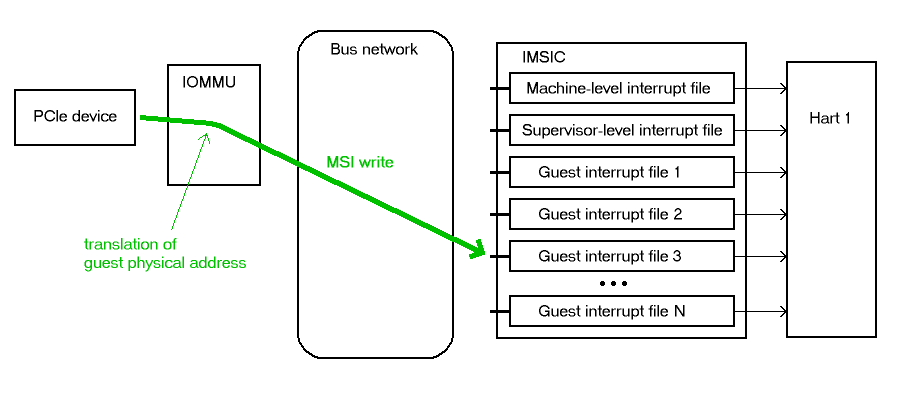
\includegraphics[scale=0.55]{IOMMU-guestIntrFiles.png}}
\caption{%
Translation of a device-sourced MSI that a guest OS intended to go to
a (virtual) IMSIC interrupt file in the OS's virtual machine.
Referencing an MSI page table supplied by the controlling hypervisor,
the \mbox{IOMMU} redirects the MSI to a guest interrupt file of the real
machine.%
}
\label{fig:IOMMU-guestIntrFiles}
\end{figure}

Memory writes from a device are recognized as MSIs by the destination
address of the write.
If an \mbox{IOMMU} determines that a \mbox{32-bit} write is to the location
of a (virtual) interrupt file in the relevant virtual machine, the
write is considered an MSI within the VM, else not.
The exact formula for recognizing MSIs is documented in
Section~\ref{sec:IOMMU-identIncomingMSIs}.

\begin{commentary}
Although the translation of MSIs is controlled by its own separate page
table, the fact that MSI translations are at the same page granularity
as regular {\RISCV} address translations implies that an address
translation cache within an \mbox{IOMMU} requires little modification to
also cache MSI translations.
Only on a translation cache miss does the \mbox{IOMMU} need to treat MSIs
significantly differently than other memory accesses from the same
device, to choose the correct translation table and to access and
interpret the table properly.
\end{commentary}

%-----------------------------------------------------------------------
\section{Memory-resident interrupt files}
\label{sec:IOMMU-MRIFs}

An \mbox{IOMMU} may optionally support memory-resident interrupt files
(MRIFs).
If implemented, the use of memory-resident interrupt files can greatly
increase the number of virtual harts that can be given direct control
of one or more physical devices in a system, assuming the rest of the
system can still handle the added load.

Without memory-resident interrupt files, the number of virtual {\RISCV}
harts that can directly receive MSIs from devices is limited by the
total number of guest interrupt files implemented by all IMSICs in the
system, because all MSIs to {\RISCV} harts must go through IMSICs.
For a single {\RISCV} hart, the number of guest interrupt files is the
\emph{GEILEN} parameter defined by the Privileged Architecture, which
can be at most 31 for RV32 and 63 for RV64.

With the use of memory-resident interrupt files, on the other hand,
the total number of virtual {\RISCV} harts able to receive device MSIs
is almost unbounded, constrained only by the amount of real physical
memory and the additional processing time needed to handle them.
As its name implies, a memory-resident interrupt file is located in
memory instead of within an IMSIC.
Figure~\ref{fig:IOMMU-MRIF} depicts how an \mbox{IOMMU} can record an
incoming MSI in an MRIF.
When properly configured by a hypervisor, an \mbox{IOMMU} recognizes certain
incoming MSIs as intended for a specific virtual interrupt file, and
records each such MSI by setting an interrupt-pending bit stored within
the MRIF data structure in ordinary memory.
After each MSI is recorded in an MRIF, the \mbox{IOMMU} also sends a
\emph{notice MSI} to the hypervisor to inform it that the MRIF contents
may have changed.

\begin{figure}[th]
\centerline{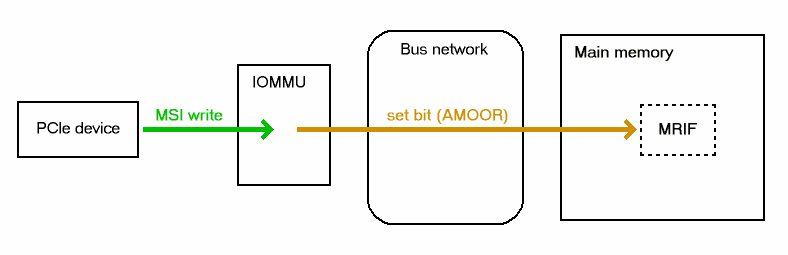
\includegraphics[scale=0.55]{IOMMU-MRIF.png}}
\caption{%
Recording an incoming MSI into a memory-resident interrupt file
(MRIF) instead of sending it to a guest interrupt file as in
Figure~\ref{fig:IOMMU-guestIntrFiles}.%
}
\label{fig:IOMMU-MRIF}
\end{figure}

While a memory-resident interrupt file provides a place to record MSIs,
it cannot interrupt a hart directly the way an IMSIC's guest interrupt
files can.
The notice MSIs that hypervisors receive only indicate that a virtual
hart \emph{might} need interrupting;
a hypervisor is responsible for examining the MRIF contents each time
to determine whether actually to interrupt the virtual hart.
Furthermore, whereas an IMSIC's guest interrupt file can directly
act as a supervisor-level interrupt file for a virtual hart, keeping
a virtual hart's interrupt file in an MRIF while the virtual hart
executes requires that the hypervisor emulate a supervisor-level
interrupt file for the virtual hart, hiding the underlying MRIF.
Depending on how often the virtual hart touches its interrupt file
and the implementation's level of support for MRIFs, the cost of this
emulation may be significant.

Consequently, MRIFs are expected most often to be used for virtual
harts that are more-or-less ``swapped out'' of a physical hart due to
being idle, or nearly so.
When a hypervisor determines that an MSI that landed in an MRIF should
wake up a particular virtual hart that was idle, the virtual hart can
be assigned a guest interrupt file in an IMSIC and its interrupt file
moved from the MRIF into this guest interrupt file before the virtual
hart is resumed.
The process of allocating a guest interrupt file for the newly wakened
virtual hart may of course force the interrupt file of another virtual
hart to be evicted to its own MRIF.

\begin{commentary}
Not all systems need to accommodate large numbers of idle virtual harts.
Many batch-processing servers, for example, strive to keep all virtual
worker threads as busy as possible from start to finish, throttled only
by I/O delays and limits on processing resources.
In such environments, support for MRIFs may not be useful, so long as
parameter GEILEN is not too small.
\end{commentary}

An \mbox{IOMMU} can have one of these three levels of support for
memory-resident interrupt files:
\begin{tightList}
\item no memory-resident interrupt files;
\item memory-resident interrupt files without atomic update; or
\item memory-resident interrupt files with atomic update.
\end{tightList}

Memory-resident interrupt files are most efficient when the memory
system supports logical atomic memory operations (AMOs) corresponding
to {\RISCV} instructions AMOAND and AMOOR, for memory accesses made
both from harts and from the \mbox{IOMMU}.
The AMOAND and AMOOR operations are required for \emph{atomic update}
of a memory-resident interrupt file.
A reduced level of support is possible without AMOs, relying solely on
basic memory reads and writes.

%- - - - - - - - - - - - - - - - - - - - - - - - - - - - - - - - - - - -
\subsection{Format of a memory-resident interrupt file}
\label{sec:IOMMU-MRIFFormat}

A memory-resident interrupt file occupies 512 bytes of memory,
naturally aligned to a \mbox{512-byte} address boundary.
The 512 bytes are organized as an array of 32 pairs of \mbox{64-bit}
doublewords, 64 doublewords in all.
Each doubleword is in little-endian byte order (even for systems where
all harts are big-endian-only).

\begin{commentary}
Big-endian-configured harts that make use of MRIFs are expected to
implement the REV8 byte-reversal instruction defined by
standard {\RISCV} extension Zbb, or pay the cost of endianness
conversion using a sequence of instructions.
\end{commentary}

The pairs of doublewords contain the interrupt-pending and
interrupt-enable bits for external interrupt identities 1--2047, in
this arrangement:
\begin{displayLinesTable}[c@{\quad}l@{\qquad}l]
offset    & \ size  & contents \\
\noalign{\medskip}
\z{0x000} & 8 bytes & interrupt-pending bits for (minor) identities 1--63 \\
\z{0x008} & 8 bytes & interrupt-enable bits for identities 1--63 \\
\z{0x010} & 8 bytes & interrupt-pending bits for identities 64--127 \\
\z{0x018} & 8 bytes & interrupt-enable bits for identities 64--127 \\
\dots     &         & \ \dots \\
\z{0x1F0} & 8 bytes & interrupt-pending bits for identities 1984--2047 \\
\z{0x1F8} & 8 bytes & interrupt-enable bits for identities 1984--2047 \\
\end{displayLinesTable}
In general, the pair of doublewords at address offsets
$k\times\mbox{16}$ and ${k\times\mbox{16}+\mbox{8}}$ for integer $k$
contain the interrupt-pending and interrupt-enable bits for external
interrupt minor identities in the range $k\times\mbox{64}$ to
$k\times\mbox{64}+\mbox{63}$.
For identity~$i$ in this range, bit $(i\bmod\mbox{64})$ of the first
(even) doubleword is the interrupt-pending bit, and the same bit of the
second (odd) doubleword is the interrupt-enable bit.

\begin{commentary}
The interrupt-pending and interrupt-enable bits are stored interleaved
by doublewords within an MRIF to facilitate the possibility of an
\mbox{IOMMU} examining the relevant enable bit to determine whether to send
a notice MSI after updating a pending bit, rather than the default
behavior of always sending a notice MSI after an update without regard
for the interrupt-enable bits.
The memory arrangement matters only when MRIFs are supported without
atomic update.
\end{commentary}

Bit~0 of the first doubleword of an MRIF stores a faux
interrupt-pending bit for nonexistent interrupt~0.
If a write from an I/O device appears to be an MSI that should be
stored in an MRIF, yet the data to write (the interrupt identity) is
zero, the \mbox{IOMMU} acts as though zero were a valid interrupt identity,
setting bit~0 of the target MRIF's first doubleword and sending a
notice MSI as usual.

All MRIFs are the size to accommodate 2047 valid interrupt identities,
the maximum allowed for an IMSIC interrupt file.
If a system's actual IMSICs have interrupt files that implement
only $N$ interrupt identities, ${N < \mbox{2047}}$, then the contents
of MRIFs for identities greater than $N$ may be ignored by software.
\mbox{IOMMU}s, however, treat every MRIF as though all interrupt identities
in the range 0--2047 are valid, even as software ignores invalid
identity~0 and all identities greater than~$N$.

\begin{commentary}
There is no need to specify to an \mbox{IOMMU} a desired size~$N$ for an
MRIF smaller than 2047 valid interrupt identities.
The only use an \mbox{IOMMU} would make of this information would be to
discard any MSIs indicating an interrupt identity greater than~$N$.
If devices are properly configured by software, such errant MSIs should
not occur;
but even if they do, it is just as effective for software to ignore
spurious interrupt identities \emph{after} they have been recorded in
an MRIF as for an \mbox{IOMMU} to discard them before recording them in the
MRIF.

It is likewise unnecessary for \mbox{IOMMU}s to check for and discard MSIs
indicating an invalid interrupt identity of zero.
\end{commentary}

%- - - - - - - - - - - - - - - - - - - - - - - - - - - - - - - - - - - -
\subsection{Recording of incoming MSIs to memory-resident interrupt files}

The data component of an MSI write specifies the interrupt identity to
raise in the destination interrupt file.
(Recall Section~\ref{sec:MSIEncoding}.)
This data may be in little-endian or big-endian byte order.
If an \mbox{IOMMU} supports memory-resident interrupt files, it can store to
an MRIF MSIs of the same endianness that the machine's IMSICs accept.
All IMSIC interrupt files are required to accept MSIs in little-endian
byte order written to memory-mapped register \z{seteipnum\_le}
(Section~\ref{sec:IMSIC-memRegion}).
IMSIC interrupt files may also accept MSIs in big-endian byte order if
register \z{seteipnum\_be} is implemented alongside \z{seteipnum\_le}.

If the interrupt identity indicated by an MSI's data (when interpreted
in the correct byte order) is in the range 0--2047, an \mbox{IOMMU} stores
the MSI to an MRIF by setting to one the interrupt-pending bit in the
MRIF for that identity.
If atomic update is supported for MRIFs, the pending bit is set using
an AMOOR operation, else it is set using a non-atomic read-modify-write
sequence.
After the interrupt-pending bit is set in the MRIF, the \mbox{IOMMU} sends
the notice MSI that software has configured for the MRIF.

The exact process of storing an MSI to an MRIF is specified more
precisely in Section~\ref{sec:IOMMU-MSIPTE-MRIF}, which covers MSI page
table entries configured in \emph{MRIF mode}.

\begin{commentary}
It is an open question whether an \mbox{IOMMU} might optionally examine
the matching interrupt-enable bit within a destination MRIF to decide
whether to send a notice MSI after setting an interrupt-pending bit.
Currently, an \mbox{IOMMU} is required always to send a notice MSI after
storing an MSI to an MRIF, even when the corresponding enable bit for
the interrupt identity is zero.
\end{commentary}

%- - - - - - - - - - - - - - - - - - - - - - - - - - - - - - - - - - - -
\subsection{Use of memory-resident interrupt files with atomic update}

To make use of a memory-resident interrupt file with support for atomic
update, software must have memory locations to save an IMSIC interrupt
file's \z{eidelivery} and \z{eithreshold} registers, in addition to the
MRIF structure itself from Section~\ref{sec:IOMMU-MRIFFormat}.

Moving a virtual hart's interrupt file from an IMSIC into an MRIF
involves these steps:
\begin{enumerate}

\item
Prepare the MRIF by zeroing all of its interrupt-pending bits (the even
doublewords) and by copying the IMSIC interrupt file's \z{eie} array to
the MRIF's interrupt-enable bits (the odd doublewords).

\item
At the IMSIC interrupt file, save to memory the existing values of
registers \z{eidelivery} and \z{eithreshold}, and set \z{eidelivery}
=~0.

\item
Modify all relevant translation tables at \mbox{IOMMU}s so that MSIs for
this virtual interrupt file are now stored in the MRIF.
If necessary, synchronize with all \mbox{IOMMU}s to ensure that no straggler
MSIs will arrive at the old IMSIC interrupt file after this step.

\item
Logically OR the contents of the IMSIC interrupt file's \z{eip} array
into the interrupt-pending bits of the MRIF, using AMOOR operations.

\end{enumerate}
Once this sequence is complete, the IMSIC interrupt file is no longer
in use.

Each time a notice MSI arrives indicating that an MSI has been
stored in the MRIF, the controlling hypervisor should scan the MRIF's
interrupt-pending and interrupt-enable bits to determine if any enabled
interrupt is now both pending and enabled and thus should interrupt the
virtual hart.

With atomic update of MRIFs, a virtual hart may continue executing
with its interrupt file contained in an MRIF, so long as the hypervisor
emulates for the virtual hart a proper IMSIC interrupt file to hide the
underlying MRIF.
Hypervisor software can safely set and clear the interrupt-pending and
interrupt-enable bits of the MRIF using AMOOR and AMOAND operations,
even as an \mbox{IOMMU} may be storing incoming MSIs into the same MRIF.

\begin{commentary}
If an \mbox{IOMMU} is ever configured to examine an MRIF's interrupt-enable
bits to decide whether to send notice MSIs, then modifying those enable
bits will generally require coordination with the \mbox{IOMMU}.
But so long as \mbox{IOMMU}s ignore the interrupt-enable bits as is
currently assumed, the bits can be changed by software without risk.
\end{commentary}

To move the same interrupt file from the MRIF back to an IMSIC:
\begin{enumerate}

\item
At the new IMSIC interrupt file, set \z{eidelivery} =~0, and zero the
\z{eip} array.

\item
Modify all relevant translation tables at \mbox{IOMMU}s so that MSIs for
this virtual interrupt file are now sent to the IMSIC interrupt file.
If necessary, synchronize with all \mbox{IOMMU}s to ensure that no straggler
MSIs will be stored in the MRIF after this step.

\item
Logically OR the interrupt-pending bits from the MRIF into the IMSIC
interrupt file, using instruction CSRS to write to the \z{eip} array.
Also, copy the interrupt-enable bits from the MRIF to the IMSIC
interrupt file's \z{eie} array.

\item
At the IMSIC interrupt file, load registers \z{eithreshold} and
\z{eidelivery} with the values that were earlier saved.

\end{enumerate}

%- - - - - - - - - - - - - - - - - - - - - - - - - - - - - - - - - - - -
\subsection{Use of memory-resident interrupt files without atomic update}

Without support for atomic update, the use of memory-resident interrupt
files is similar to the atomic-update case of the previous subsection,
but with some added complexities.

First, if the I/O devices that a virtual hart controls are behind
multiple \mbox{IOMMUs}, then multiple MRIF structures are needed, one per
\mbox{IOMMU}, not just a single MRIF structure.
Furthermore, in addition to locations for storing \z{eidelivery} and
\z{eithreshold}, software needs a place for a complete copy of the
interrupt file's implemented \z{eip} array, apart from the MRIFs.
While a virtual interrupt file is in memory, its interrupt-pending bits
will be split across all the MRIFs and the saved \z{eip} array.
The interrupt-enable bits will exist only in the MRIFs.

To move a virtual hart's interrupt file from an IMSIC into memory, with
one MRIF per \mbox{IOMMU}:
\begin{enumerate}

\item
Prepare all MRIFs by zeroing their interrupt-pending bits (the even
doublewords) and by copying the IMSIC interrupt file's \z{eie} array to
the MRIFs' interrupt-enable bits (the odd doublewords).

\item
At the IMSIC interrupt file, save to memory the existing values of
registers \z{eidelivery} and \z{eithreshold}, and set \z{eidelivery}
=~0.

\item
At each \mbox{IOMMU}, modify all relevant translation tables so that MSIs
for this virtual interrupt file are now stored in the individual MRIF
matched to the \mbox{IOMMU}.
If necessary, synchronize with all \mbox{IOMMU}s to ensure that no straggler
MSIs will arrive at the old IMSIC interrupt file after this step.

\item
Dump the IMSIC interrupt file's \z{eip} array to its separate location
outside the MRIFs.

\end{enumerate}
Once this sequence is complete, the IMSIC interrupt file is no longer
in use.

While a virtual hart's interrupt file remains in memory, an interrupt
identity's true pending bit is the logical OR of its bit in all MRIFs
and its bit in the saved \z{eip} array.
All pending bits in the MRIFs start as zeros, but interrupts may become
pending there as MSIs for this virtual hart arrive at \mbox{IOMMU}s and are
stored in the corresponding MRIFs.

Without atomic update of MRIFs, an interrupt-pending bit is not easily
cleared in an MRIF.
(Clearing a single pending bit in one MRIF requires that a new MRIF be
allocated and initialized and the corresponding \mbox{IOMMU} reconfigured to
store MSIs into the new MRIF.)
For this reason, it may or may not be practical to have a virtual hart
execute while keeping one of its interrupt files in memory.
When an MRIF records an interrupt that should wake a virtual hart, the
simplest strategy is to always move the interrupt file back into an
IMSIC's guest interrupt file before resuming execution of the virtual
hart.

To transfer an interrupt file from memory back to an IMSIC:
\begin{enumerate}

\item
At the new IMSIC interrupt file, set \z{eidelivery} =~0, and zero the
\z{eip} array.

\item
Modify all relevant translation tables at \mbox{IOMMU}s so that MSIs for
this virtual interrupt file are now sent to the IMSIC interrupt file.
If necessary, synchronize with all \mbox{IOMMU}s to ensure that no straggler
MSIs will be stored in MRIFs after this step.

\item
Merge by bitwise logical OR the interrupt-pending bits of all MRIFs and
the saved \z{eip} array, and logically OR these merged bits into the
IMSIC interrupt file, using instruction CSRS to write to the \z{eip}
array.
Also, copy the interrupt-enable bits from one of the MRIFs to the IMSIC
interrupt file's \z{eie} array.

\item
At the IMSIC interrupt file, load registers \z{eithreshold} and
\z{eidelivery} with the values that were earlier saved.

\end{enumerate}

%- - - - - - - - - - - - - - - - - - - - - - - - - - - - - - - - - - - -
\subsection{Allocation of guest interrupt files for receiving notice MSIs}

The processing a hypervisor does in response to notice MSIs can be
minimized by assigning a separate interrupt identity for each MRIF, so
the identity encoded in a notice MSI always indicates which one MRIF
may have changed.
However, if there are very many MRIFs (potentially in the thousands),
a hypervisor may run short of interrupt identities within the
supervisor-level interrupt files available in IMSICs.
In that case, the hypervisor can increase its supply of interrupt
identities by allocating one or more of the IMSICs' guest interrupt
files to itself for the purpose of receiving notice MSIs.

\begin{commentary}
Although guest interrupt files exist primarily to act as
supervisor-level interrupt files for virtual harts, the IMSIC hardware
does not police exactly how they are used by software.
\end{commentary}

%-----------------------------------------------------------------------
\section{Identification of incoming MSIs for a virtual machine}
\label{sec:IOMMU-identIncomingMSIs}

When an I/O device is configured directly by a guest operating system,
MSIs from the device are expected to be targeted to virtual IMSICs
within the guest OS's virtual machine, using guest physical addresses
that are inappropriate and unsafe for the real machine.
An \mbox{IOMMU} must recognize certain incoming writes from such devices as
MSIs and convert them as needed for the real machine.
(Recall Figure~\ref{fig:IOMMU-guestIntrFiles}.)

MSIs originating from a single device that require conversion are
expected to have been configured at the device by a single guest OS
running within one {\RISCV} virtual machine.
Assuming the VM itself conforms to the Advanced Interrupt Architecture,
MSIs are sent to virtual harts within the VM by writing to the
memory-mapped registers of the interrupt files of virtual IMSICs.
Each of these virtual interrupt files occupies a separate \mbox{4-KiB}
page in the VM's guest physical address space, the same as real
interrupt files do in a real machine's physical address space.
A write to a guest physical address can thus be recognized as an MSI to
a virtual hart if the write is to a page occupied by an interrupt file
of a virtual IMSIC within the VM.

The MSI address mask and address pattern specified in a device context
(Section~\ref{sec:IOMMU-deviceContexts}) are used to identify the
\mbox{4-KiB} pages of virtual interrupt files in the guest physical
address space of the relevant VM.
An incoming \mbox{32-bit} write made by a device is recognized as an
MSI write to a virtual interrupt file if the destination guest physical
page matches the supplied address pattern in all bit positions that are
zeros in the supplied address mask.
In detail, a write to guest physical address~$A$ is recognized as an
MSI to a virtual interrupt file if
$$
\bigl(\mbox{($A$\,\z{>>}\,12) \z{\&} $\sim$address mask}\bigr)
  = (\mbox{address pattern \z{\&} $\sim$address mask})
$$
where \mbox{\z{>>}\,12} represents shifting right by 12~bits,
an ampersand (\z{\&}) represents bitwise logical AND, and
``$\sim$address mask'' is the bitwise logical complement of the address
mask.

When a write is identified as an MSI from a device, an
\emph{interrupt file number} is extracted from the original guest
physical address as
\begin{displayLinesTable}
interrupt file number = extract($A$\,\z{>>}\,12, address mask) \\
\end{displayLinesTable}
The extract function here is the same generic bit extract performed
by {\RISCV} instruction BEXT, defined by the ``Bitmanip'' extension
(B~extension).
The bit extract function extract($x$,~$y$) discards all bits from
$x$ whose matching bits in the same positions in the mask~$y$ are
zeros, and packs the remaining bits from $x$ contiguously at the
least-significant end of the result, keeping the same bit order as $x$
and filling any other bits at the most-significant end of the result
with zeros.
For example, if the bits of $x$ and $y$ are
\begin{displayLinesTable}[r@{ }c@{ }c@{ }c@{ }c@{ }c@{ }c@{ }c@{ }c]
$x$ = & a & b & c & d & e & f & g & h \\
$y$ = & 1 & 0 & 1 & 0 & 0 & 1 & 1 & 0 \\
\end{displayLinesTable}
then the value of extract($x$,~$y$) has bits 0~0~0~0~a~c~f~g.

%-----------------------------------------------------------------------
\section{MSI page tables}

Whenever an \mbox{IOMMU} recognizes an incoming write from a device as
an MSI by the method specified in the previous section, the MSI is
translated or converted by consulting the MSI page table configured for
the device, instead of using the regular translation data structures
that apply to all other memory accesses from the same device.

Only naturally aligned \mbox{32-bit} writes from a device are possible
MSIs.
For other forms of memory accesses by a device (such as reads, writes
of other sizes, or misaligned writes), the regular translation data
structures are always applied, even if the address matches that of a
proper MSI.

An MSI page table is a flat array of MSI page table entries (MSI PTEs),
each 16~bytes.
MSI page tables have no multi-level hierarchy like regular {\RISCV}
page tables do.
Rather, every MSI PTE is a leaf entry specifying the translation or
conversion of writes made to a particular \mbox{4-KiB} guest physical
page that a virtual interrupt file occupies (or may occupy) in the
relevant virtual machine.
To select an individual MSI PTE from an MSI page table, the PTE array
is indexed by the interrupt file number extracted from the destination
guest physical address of the incoming MSI write by the formula of the
previous section.
Each MSI PTE may specify either the address of a real guest interrupt
file that substitutes for the targeted virtual interrupt file (as in
Figure~\ref{fig:IOMMU-guestIntrFiles}), or a memory-resident interrupt
file in which to store incoming MSIs for the virtual interrupt file
(as in Figure~\ref{fig:IOMMU-MRIF}).

The number of entries in an MSI page table is always a power of two,
specifically $\mbox{2}^{k}$ where $k$ is the number of bits that are
ones in the MSI address mask used to extract the interrupt file number
from the destination guest physical address.
If an MSI page table has 256 or fewer entries, the start of the table
is always aligned to a \mbox{4-KiB} page address in real physical
memory.
If an MSI page table has ${\mbox{2}^{k} > \mbox{256}}$
entries, the table must be naturally aligned to a
$\mbox{2}^{k}\times \mbox{16-byte}$ address boundary.
If an MSI page table is not aligned as required, all entries in the
table appear to an \mbox{IOMMU} as {\unspecified}, and any address an
\mbox{IOMMU} may compute and use for reading an individual MSI PTE from the
table is also {\unspecified}.

Every \mbox{16-byte} MSI PTE is interpreted as two \mbox{64-bit}
doublewords.
If an \mbox{IOMMU} also references standard {\RISCV} page tables, defined by
the {\RISCV} Privileged Architecture, for regular address translation,
then the byte order for each of the two doublewords in memory,
little-endian or big-endian, should be the same as the endianness
of the regular {\RISCV} page tables configured for the same device
context.
Otherwise, the endianness of the doublewords of an MSI PTE is
implementation-defined.

Bit~0 of the first doubleword of an MSI PTE is field~V (Valid).
When V~=~0, the PTE is invalid, and all other bits of both doublewords
are ignored by an \mbox{IOMMU}, making them free for software to use.

If V~=~1, bit~63 of the first doubleword is field~C (Custom),
designated for custom use.
If an MSI PTE has V~=~1 and C~=~1, interpretation of the rest of the
PTE is implementation-defined.

If V~=~1 and the custom-use bit C~=~0, then bit~2 of the first
doubleword is field~W (Write-through).
If W~=~1, the MSI PTE specifies \emph{write-through mode} for incoming
MSIs, and if W~=~0, it specifies \emph{MRIF mode}.
The interpretation of an MSI PTE for each of these two modes is
detailed further in the next two subsections.

%- - - - - - - - - - - - - - - - - - - - - - - - - - - - - - - - - - - -
\subsection{MSI PTE, write-through mode}

When an MSI PTE has fields V~=~1, C~=~0, and W~=~1
(write-through mode), the PTE's complete format is:\nopagebreak
\begin{displayLinesTable}[l@{\quad}l@{\quad}l]
First doubleword:  & bit 63     & C, = 0 \\
                   & bits 53:10 & PPN \\
                   & bit 2      & W, = 1 \\
                   & bit 0      & V, = 1 \\
\noalign{\medskip}
Second doubleword: & ignored \\
\end{displayLinesTable}
All other bits of the first doubleword are reserved and must be set to
zeros by software.
The second doubleword is ignored by an \mbox{IOMMU} so is free for software
to use.

An incoming MSI write is translated by replacing the write's original
address bits 12 and above (the guest physical page number) with field
PPN (Physical Page Number) from the PTE, while retaining the original
address bits 11:0 (the page offset).
This translated address is either zero-extended or clipped at the upper
end as needed to make it the width of a real physical address for the
machine.
The original memory write from the device is then passed onward to the
memory system with the new address.

An MSI PTE in write-through mode allows a hypervisor to route an
MSI intended for a virtual interrupt file to go instead to a guest
interrupt file of a real IMSIC in the machine.

\begin{commentary}
An \mbox{IOMMU} that also employs standard {\RISCV} page tables for regular
address translation can maximize the overlap between the handling of
MSI PTEs and regular {\RISCV} leaf PTEs as follows:

For RV64, the first doubleword of an MSI PTE in write-through mode
has the same encoding as a regular {\RISCV} leaf PTE for Sv39, Sv48,
Sv39x4, or Sv48x4 page-based address translation, with PTE fields D, A,
G, U, X, and R all zeros and W~=~1.
Hence, the MSI PTE's first doubleword appears the same as a regular
PTE that grants write permission (W~=~1) but not read or execute
permissions (X~= R =~0).
This same-encoded regular PTE would translate an MSI write the same as
the actual MSI PTE, except that what would be the PTE's accessed (A),
dirty (D), and user (U) bits are all zeros.
An \mbox{IOMMU} needs to treat only these three bits differently for an MSI
PTE versus a regular RV64 leaf PTE.

The address computation used to select a PTE from a regular {\RISCV}
page table must be modified to select an MSI PTE's first doubleword
from an MSI page table.
However, the extraction of an interrupt file number from a guest
physical address to obtain the index for accessing the MSI page table
already creates an unavoidable difference in PTE addressing.

For RV32, the lower \mbox{32-bit} word of an MSI PTE's first doubleword
has the same format as a leaf PTE for Sv32 or Sv32x4 page-based address
translation, except again for what would be PTE bits A, D, and~U, which
must be treated differently.
\end{commentary}

%- - - - - - - - - - - - - - - - - - - - - - - - - - - - - - - - - - - -
\subsection{MSI PTE, MRIF mode}
\label{sec:IOMMU-MSIPTE-MRIF}

If memory-resident interrupt files are supported and an MSI PTE has
fields V~=~1, C~=~0, and W~=~0 (MRIF mode), the PTE's complete format
is:\nopagebreak
\begin{displayLinesTable}[l@{\quad}l@{\quad}l]
First doubleword:  & bit 63     & C, = 0 \\
                   & bits 53:7  & MRIF Address[55:9] \\
                   & bit 2      & W, = 0 \\
                   & bit 0      & V, = 1 \\
\noalign{\medskip}
Second doubleword: & bit 60     & NID[10] \\
                   & bits 53:10 & NPPN \\
                   & bits 9:0   & NID[9:0] \\
\end{displayLinesTable}
All other PTE bits are reserved and must be set to zeros by software.

The PTE's MRIF Address field provides bits 55:9 of the physical address
of a memory-resident interrupt file in which to store incoming MSIs,
referred to as the \emph{destination MRIF}.
As every memory-resident interrupt file is naturally aligned to a
\mbox{512-byte} address boundary, bits 8:0 of the destination MRIF's
address must be zero and are not specified in the PTE.

Field NPPN (Notice Physical Page Number) and the two NID
(Notice Identifier) fields together specify a destination and value for
a \emph{notice MSI} that is sent after each time the destination MRIF
is updated as a result of consulting this PTE to store an incoming MSI.

\begin{commentary}
Typically, NPPN will be the page address of an IMSIC's interrupt file
in the real machine, and NID will be the interrupt identity to make
pending in that interrupt file to indicate that the destination MRIF
may have changed.
However, NPPN is not required to be a valid interrupt file address, and
an \mbox{IOMMU} must not attempt to restrict it to only such addresses.
Any page address must be accepted for NPPN.
\end{commentary}

When the IMSIC interrupt files in the system implement memory-mapped
register \z{seteipnum\_be} for receiving MSIs in big-endian byte order
(Section~\ref{sec:IMSIC-memRegion}), then an \mbox{IOMMU} must be able to
store MSIs in both little-endian and big-endian byte orders to the
destination MRIF.
If the IMSIC interrupt files in the system do not implement
register \z{seteipnum\_be}, an \mbox{IOMMU} should ordinarily store only
little-endian MSIs to the destination MRIF.
The data of an incoming MSI is assumed to be in little-endian byte
order if bit~2 of the destination address is zero, and in big-endian
byte order if bit~2 of the destination address is one.

If the incoming MSI write is to guest physical address~$A$ and its
\mbox{32-bit} data is~$D$ when interpreted in the byte order indicated
by bit~2 of $A$, then the MSI is processed by the \mbox{IOMMU} as follows:
If either $A$\z{[}11:3\z{]} or $D$\z{[}31:11\z{]} is not zero, or if
bit~2 of $A$ is one and big-endian MSIs are not supported, then the
incoming write is accepted but discarded.
Else, the original incoming write is replaced by this sequence:
\begin{enumerate}

\item
In the destination MRIF, set the interrupt-pending bit for interrupt
identity $D$ to one, using either an AMOOR operation for atomic update,
or a non-atomic read-modify-write sequence.

\item
Zero-extend the \mbox{11-bit} NID value to 32~bits, and do a
\mbox{32-bit} write of this value in little-endian byte order to the
address NPPN\,\z{<<}\,12 (i.e., physical page number NPPN, page offset
zero).

\end{enumerate}
The write of step~1 must be visible to all agents in the system before
the write of step~2 becomes visible to any agent.

\begin{commentary}
While \mbox{IOMMU}s are expected typically to cache MSI PTEs that are
configured in write-through mode (W~=~1), they might not cache PTEs
configured in MRIF mode (W~=~0).
Two reasons together justify not caching MSI PTEs in MRIF mode:
First, the information and actions required to store an MSI to an MRIF
are far different than normal address translation; and
second, by their nature, MSIs to MRIFs should occur less frequently.
Hence, an \mbox{IOMMU} might perform MRIF-mode processing solely as
an extension of cache-miss page table walks, leaving its address
translation cache oblivious to MRIF-mode MSI PTEs.
\end{commentary}



%=======================================================================

\end{document}

